% ==========================================================
%  ML UNSUPERVISED TECHNIQUES — MASTER SUMMARY
%  Based on: Hochreiter, Machine Learning: Unsupervised Methods, JKU Linz
% ==========================================================

\documentclass[11pt, oneside]{book}

\usepackage[
  a4paper,
  top    = 2.6cm,
  bottom = 2.1cm,
  left   = 2.5cm,
  right  = 2.5cm,
  headheight = 15pt
]{geometry}

\usepackage[T1]{fontenc}
\usepackage[utf8]{inputenc}
\usepackage{lmodern}
\usepackage{microtype}
\usepackage{inconsolata}

\setlength{\parindent}{0pt}
\setlength{\parskip}{0.62em}

\usepackage{amsmath, amssymb, amsthm, mathtools}
\usepackage{bm}
\usepackage{bbm}
\usepackage{mathrsfs}
\usepackage{nicefrac}
\usepackage{cancel}

\usepackage{siunitx}
\sisetup{per-mode = symbol}

\usepackage{graphicx}
\usepackage{booktabs}
\usepackage{array}
\usepackage{float}
\usepackage{enumitem}

\setlist[itemize]{topsep=3pt, itemsep=2pt, leftmargin=2.2em}
\setlist[enumerate]{topsep=3pt, itemsep=2pt, leftmargin=2.4em}

\usepackage[ruled, vlined, linesnumbered]{algorithm2e}
\SetAlFnt{\small}
\SetAlCapFnt{\small\bfseries}
\SetCommentSty{textit}

\usepackage{xcolor}

\definecolor{accent}{HTML}{1B3A5C}
\definecolor{def@frame}{HTML}{1A5276}   \definecolor{def@bg}{HTML}{EBF5FB}
\definecolor{thm@frame}{HTML}{922B21}   \definecolor{thm@bg}{HTML}{FDEDEC}
\definecolor{ex@frame} {HTML}{1E8449}   \definecolor{ex@bg} {HTML}{EAFAF1}
\definecolor{int@frame}{HTML}{9A6A00}   \definecolor{int@bg}{HTML}{FEF9E7}
\definecolor{note@frame}{HTML}{5B2C6F}  \definecolor{note@bg}{HTML}{F5EEF8}

\usepackage{listings}
\lstset{
  basicstyle       = \ttfamily\small,
  breaklines       = true,
  numbers          = left,
  numberstyle      = \tiny\color{gray!70},
  frame            = tb,
  framerule        = 0.4pt,
  rulecolor        = \color{gray!35},
  tabsize          = 2,
  showstringspaces = false,
  keywordstyle     = \color{def@frame}\bfseries,
  commentstyle     = \color{gray!55!black}\itshape,
  stringstyle      = \color{ex@frame!90!black},
  backgroundcolor  = \color{gray!5},
  xleftmargin      = 2em,
  xrightmargin     = 0.4em,
  aboveskip        = 0.8em,
  belowskip        = 0.5em
}

\usepackage[most]{tcolorbox}

\tcbset{
  enhanced,
  breakable,
  arc             = 2.5mm,
  boxrule         = 0.5pt,
  left            = 4.5mm,
  right           = 4mm,
  top             = 2.5mm,
  bottom          = 2.5mm,
  fonttitle       = \bfseries\small,
  sharp corners   = west,
  parbox          = false
}

\newtcolorbox{defbox}[1][]{
  title  = {Definition},
  colback = def@bg, colframe = def@frame,
  borderline west = {3.5pt}{0pt}{def@frame},
  #1
}

\newtcolorbox{thmbox}[1][]{
  title  = {Theorem / Key Formula},
  colback = thm@bg, colframe = thm@frame,
  borderline west = {3.5pt}{0pt}{thm@frame},
  #1
}

\newtcolorbox{exbox}[1][]{
  title  = {Example},
  colback = ex@bg, colframe = ex@frame,
  borderline west = {3.5pt}{0pt}{ex@frame},
  #1
}

\newtcolorbox{intbox}[1][]{
  title  = {Intuition \& Mental Model},
  colback = int@bg, colframe = int@frame,
  borderline west = {3.5pt}{0pt}{int@frame},
  #1
}

\newtcolorbox{notebox}[1][]{
  title  = {Note},
  colback = note@bg, colframe = note@frame,
  borderline west = {3.5pt}{0pt}{note@frame},
  #1
}

% Compile-safe marker for visuals that should be added later.  Keeping the
% description and search terms in the source makes replacing the marker with an
% actual \includegraphics command straightforward.
\newcommand{\figureplaceholder}[3]{%
\begin{figure}[H]
  \centering
  \begin{tcolorbox}[
    width=.94\linewidth,
    breakable=false,
    colback=gray!4,
    colframe=accent!55,
    title={Visual to add},
    borderline west={3.5pt}{0pt}{accent!55}
  ]
    \raggedright
    \textbf{What the figure should show:} #2

    \smallskip
    \textbf{Good search query:} \texttt{#3}
  \end{tcolorbox}
  \caption{#1}
\end{figure}
}

\usepackage[titles]{tocloft}

\renewcommand{\cftchapfont}     {\bfseries\color{accent}}
\renewcommand{\cftchappagefont} {\bfseries\color{accent}}
\renewcommand{\cftchapleader}   {\bfseries\color{accent!40}\cftdotfill{\cftdotsep}}
\setlength{\cftbeforechapskip} {7pt}

\renewcommand{\cftsecfont}      {\small}
\renewcommand{\cftsecpagefont}  {\small}
\setlength{\cftsecindent}      {1.8em}
\setlength{\cftbeforesecskip}  {1.5pt}

\renewcommand{\cftsubsecfont}      {\small\color{gray!65!black}}
\renewcommand{\cftsubsecpagefont}  {\small\color{gray!65!black}}
\setlength{\cftsubsecindent}      {3.4em}
\setlength{\cftbeforesubsecskip}  {0.5pt}

\usepackage{titlesec}

\titleformat{\chapter}[display]
  {\normalfont\bfseries\color{accent}\huge}
  {\hfill\fontsize{68}{68}\selectfont\color{accent!13}\thechapter}
  {-10pt}
  {}
  [{\vspace{4pt}%
    {\color{accent}\rule{\linewidth}{1.6pt}}\\[-2pt]%
    {\color{accent!35}\rule{\linewidth}{0.5pt}}}]
\titlespacing*{\chapter}{0pt}{-28pt}{22pt}

\titleformat{\section}
  {\normalfont\large\bfseries\color{accent}}
  {\thesection}
  {0.8em}
  {}
  [{\vspace{1pt}\color{accent!45}\titlerule[0.45pt]}]
\titlespacing*{\section}{0pt}{3.8ex plus 1ex minus .2ex}{2.2ex plus .2ex}

\titleformat{\subsection}
  {\normalfont\normalsize\bfseries\color{accent!80!black}}
  {\thesubsection}
  {0.7em}
  {}
\titlespacing*{\subsection}{0pt}{2.6ex plus 1ex minus .2ex}{1.4ex plus .2ex}

\titleformat{\paragraph}[runin]
  {\normalfont\small\bfseries}
  {}
  {0em}
  {}[.\enspace]
\titlespacing{\paragraph}{0pt}{1.2ex plus .5ex minus .2ex}{0.5em}

\usepackage{fancyhdr}
\pagestyle{fancy}
\fancyhf{}
\fancyhead[L]{\small\color{gray!70}\nouppercase{\leftmark}}
\fancyhead[R]{\small\color{gray!70}\thepage}
\renewcommand{\headrulewidth}{0.4pt}

\fancypagestyle{plain}{%
  \fancyhf{}
  \fancyfoot[C]{\small\color{gray!70}\thepage}
  \renewcommand{\headrulewidth}{0pt}%
}

\usepackage[hidelinks]{hyperref}
\usepackage[nameinlink, capitalize]{cleveref}


% ══════════════════════════════════════════════════════════
%  DOCUMENT METADATA
% ══════════════════════════════════════════════════════════
\newcommand{\coursetitle}{ML Unsupervised Techniques}
\newcommand{\documenttype}{Master Summary}
\newcommand{\authorname}{Stefan Eder}
\newcommand{\basedon}{Based on Hochreiter, \emph{Machine Learning: Unsupervised Methods}, JKU Linz}


% ══════════════════════════════════════════════════════════
%  MATHEMATICAL MACROS
% ══════════════════════════════════════════════════════════

% ── Number Sets ───────────────────────────────────────────
\newcommand{\R}{\mathbb{R}}
\newcommand{\N}{\mathbb{N}}
\newcommand{\Z}{\mathbb{Z}}
\newcommand{\C}{\mathbb{C}}

% ── Probability & Statistics ──────────────────────────────
\newcommand{\E}{\mathbb{E}}
\newcommand{\Prob}{\mathbb{P}}
\newcommand{\Var}{\mathrm{Var}}
\newcommand{\Cov}{\mathrm{Cov}}
\newcommand{\iid}{\overset{\mathrm{iid}}{\sim}}
\newcommand{\ind}{\mathbbm{1}}

% ── Information Theory ────────────────────────────────────
\newcommand{\KL}[2]{D_{\mathrm{KL}}\!\left(#1 \,\|\, #2\right)}
\newcommand{\Ent}{\mathrm{H}}
\newcommand{\MI}{\mathrm{I}}

% ── Calculus & Optimization ───────────────────────────────
\newcommand{\argmax}{\operatorname*{arg\,max}}
\newcommand{\argmin}{\operatorname*{arg\,min}}
\newcommand{\grad}{\nabla}
\newcommand{\dd}{\,\mathrm{d}}
\newcommand{\pd}[2]{\frac{\partial #1}{\partial #2}}
\newcommand{\pdd}[2]{\frac{\partial^2 #1}{\partial #2^2}}

% ── Linear Algebra ────────────────────────────────────────
\newcommand{\T}{^{\top}}
\newcommand{\inv}{^{-1}}
\newcommand{\tr}{\mathrm{tr}}
\newcommand{\diag}{\mathrm{diag}}
\newcommand{\norm}[1]{\left\lVert #1 \right\rVert}
\newcommand{\abs}[1]{\left\lvert #1 \right\rvert}
\newcommand{\inner}[2]{\left\langle #1,\, #2 \right\rangle}

% ── Course-specific notation ──────────────────────────────
% Parameter vector and estimate
\newcommand{\wvec}{\bm{w}}
\newcommand{\what}{\hat{\bm{w}}}
% Data vector and matrix
\newcommand{\xvec}{\bm{x}}
\newcommand{\Xmat}{\bm{X}}
% Latent / source variable
\newcommand{\uvec}{\bm{u}}
% Likelihood and free energy
\newcommand{\lhood}{\mathcal{L}}
\newcommand{\Fbound}{\mathcal{F}}
% MSE and bias operators
\newcommand{\mse}{\mathrm{mse}}
\newcommand{\bias}{b}
% Distributions
\newcommand{\Normal}{\mathcal{N}}

% ── Misc ─────────────────────────────────────────────────
\newcommand{\given}{\,\vert\,}
\newcommand{\st}{\;\text{s.t.}\;}
\newcommand{\eqdef}{\coloneqq}


% ==========================================================
%  BEGIN DOCUMENT
% ==========================================================
\begin{document}

\frontmatter


% ── Title Page ────────────────────────────────────────────
\thispagestyle{empty}
\vspace*{1.8cm}

\begin{center}
  {\color{accent}\rule{\linewidth}{1.8pt}}
  \vspace{0.65cm}

  {\fontsize{28}{34}\selectfont\bfseries\color{accent}\coursetitle\par}
  \vspace{0.25cm}
  {\large\color{gray!80!black}\documenttype\par}

  \vspace{0.55cm}
  {\color{accent!35}\rule{\linewidth}{0.5pt}}
  \vspace{0.55cm}

  {\large\authorname\par}
  \vspace{0.2cm}
  {\small\color{gray!70}\basedon\par}
\end{center}

\vspace{1.6cm}

\begin{center}
\begin{minipage}{0.84\textwidth}
  \small\color{gray!80!black}
  This document is a summary of the course, written to be \emph{understood} rather
  than merely consulted: the prose tries to explain why each method works before
  it states what it does, and the coloured boxes flag the definitions, key
  formulas, worked examples, mental models, and exam traps.
  Long proofs are condensed or omitted in favour of clarity.
  Use it as a study aid alongside the lecture notes and slides, not as a
  replacement for them.

  \medskip
  If you spot an error or a gap, please open an issue or pull request at
  \textbf{github.com/stevetgit} --- corrections are always welcome.

  \medskip
  \color{gray!60!black}
  Good study materials should be shared, not gatekept.
  If this helped you, take it as a reason to help the next colleague you see struggling with something.
\end{minipage}
\end{center}

\vfill
{\centering\small\color{gray!65} Compiled \today\par}
\clearpage


% ── Table of Contents ─────────────────────────────────────
\setcounter{tocdepth}{2}

\begingroup
  \let\cleardoublepage\relax
  \let\clearpage\relax
  \tableofcontents
\endgroup

\mainmatter


% ==========================================================
\chapter{Introduction}
% ==========================================================

\section{Machine Learning Introduction}

Machine learning is currently a major research topic in academia and industry alike.
Applications span computer vision, speech recognition, recommender systems, and the
analysis of large biological datasets.
In the biomedical context, modern measurement technologies --- mRNA concentrations
measured via microarrays or next-generation sequencing, SNP arrays, copy number
variation data --- create a demand for methods that can extract structure from
high-dimensional data without relying on labeled training examples.

The machine learning course series at JKU Linz comprises four complementary courses:
\begin{itemize}
  \item \textbf{Basic Methods of Data Analysis:} summary statistics, PCA, ICA,
        multidimensional scaling, clustering, biclustering.
  \item \textbf{ML Supervised Methods:} classification and regression, SVMs, neural
        networks, deep learning, LSTM, ARMA/ARIMA.
  \item \textbf{ML Unsupervised Methods} (this course): MLE, MAP, maximum entropy,
        EM, PCA, ICA, factor analysis, mixture models, HMMs, Boltzmann machines.
  \item \textbf{Theoretical Concepts of Machine Learning:} estimation theory,
        VC-dimension, generalization bounds, convex optimization, Bayes theory.
\end{itemize}

The goal is not only to know individual methods, but to be able to \emph{choose}
the right approach for a given problem, understand the mathematical foundations well
enough to adapt standard algorithms, and recognize when a model is likely to fail.


\section{Course Specific Introduction}

A learning problem is called \emph{unsupervised} when the training data contain no
target label or desired output. The algorithm must discover useful structure from the
observations themselves. That makes evaluation less direct than in supervised learning:
there is usually no single per-sample answer to compare against. Depending on the goal,
we therefore inspect held-out likelihood, reconstruction error, cluster stability,
neighbourhood preservation, or whether the representation helps a downstream task.
Modern generative models such as VAEs and diffusion models belong to this broad family,
although they use additional ideas beyond the classical methods in this script.

\paragraph{Objectives} Unsupervised methods are driven by different optimality criteria,
depending on the problem:
\begin{itemize}
  \item information content (maximizing information preserved after projection)
  \item orthogonality of extracted components
  \item statistical independence of components
  \item explained variance
  \item entropy of the representation
  \item likelihood: probability that the model produces the observed data
  \item distances within and between clusters
\end{itemize}

\paragraph{Use cases} Unsupervised methods are used to:
explore data, find latent structure, visualize high-dimensional data in low dimensions,
and compress representations.
The unifying goal is to \emph{understand and explore the data and generate new knowledge}.

\paragraph{Key concepts in this course}
Maximum likelihood (ML), maximum a posteriori (MAP), maximum entropy, expectation
maximization (EM), maximal variance, statistical independence, non-Gaussianity,
sub- and super-Gaussian distributions, sparse codes and population codes.

\paragraph{Model selection and overfitting}
The goal of learning is to select, from a model class, the model with the highest
\emph{generalization performance} --- the model that best explains \emph{future} data.
These terms should not be conflated. \emph{Training} estimates parameters for a fixed
model and objective; \emph{model selection} chooses hyperparameters or even a model
family, ideally using held-out data; \emph{learning} is the umbrella term for both.
\emph{Overfitting} occurs when the model is fitted to idiosyncratic training
characteristics (noise, outliers, labeling errors) rather than to the true underlying
structure; the model has high training performance but poor generalization.

\begin{intbox}
  Underfitting (model too simple) and overfitting (model too complex) are the two
  failure modes. The goal is the best bias-variance trade-off: a model complex enough
  to capture the true structure but not so complex that it memorizes noise.
\end{intbox}

\paragraph{Parametric vs.\ nonparametric models}
An important early decision is the \emph{model class}:

\begin{itemize}
  \item \textbf{Parametric models:} each parameter vector $\wvec$ represents one model.
        Examples: neural networks (synaptic weights), SVMs (weight vector $\wvec$), factor
        analysis. Learning corresponds to a path through parameter space.
        Disadvantages: different parameterizations can represent the same function; model
        complexity is implicitly controlled through the parameters.

  \item \textbf{Nonparametric models:} their effective number of parameters can grow
        with the amount of data. Examples are $k$-nearest neighbours, kernel density
        estimation, and many decision-tree methods. ``Nonparametric'' does \emph{not}
        mean ``has no parameters'': choices such as $k$, bandwidth, or tree depth still
        matter and are commonly selected from data by validation.
\end{itemize}

\paragraph{Unsupervised methods covered in this course}
Principal component analysis (PCA), independent component analysis (ICA), factor analysis,
projection pursuit, $k$-means clustering, hierarchical clustering, mixture models
(Gaussian, Poisson), self-organizing maps (SOMs), kernel density estimation, hidden Markov
models (HMMs, factorial HMMs, IO-HMMs), Markov networks, restricted Boltzmann machines,
auto-associators.

Methods fall into two broad families:
\begin{itemize}
  \item \textbf{Projection methods:} produce a new representation of objects by
        down-projecting feature vectors into a lower-dimensional space while preserving
        neighborhoods or other desired properties.
        Examples: PCA (orthogonal components of maximal variance) and ICA (statistically
        independent components). Factor analysis is related but is better viewed as a
        probabilistic latent-variable model with an explicit noise model.
  \item \textbf{Generative models:} build an explicit probabilistic model of the observed
        data; the fitted model should match the observed data density.
\end{itemize}


\section{Generative vs.\ Descriptive Models}
\label{sec:gen-vs-desc}

\begin{defbox}[title={Descriptive (Recoding) Model}]
A \textbf{descriptive model} doesn't try to explain where the data \emph{came from} ---
it just re-describes it in a more useful form. It maps each observation into a new space
with some desired property baked in: uncorrelated axes (PCA) or statistically independent
ones (ICA).
\end{defbox}

\begin{defbox}[title={Generative Model}]
A \textbf{generative model} goes the other way: it models \emph{how the data was made}.
The story is that hidden source components $\uvec$ are drawn from a prior $p_{\uvec}$,
pushed through a model $g(\uvec;\wvec)$, and out comes the data. Training then tunes
$\wvec$ so that the model's distribution $p(\xvec;\wvec)$ matches what we actually
observe, $p(\xvec)$.
Examples: factor analysis, latent variable models, Boltzmann machines, HMMs.
\end{defbox}

Generative models allow the use of prior knowledge about the world and enable the
prediction of new states of the data-generating process (e.g.\ predicting gene expression
or brain activity). The natural training objective is maximum likelihood or MAP.

Descriptive models aim to find a richer or more interpretable representation rather than
to model the generative process.
Their objectives are properties of the representation: maximal variance (PCA),
statistical independence (ICA), maximal non-Gaussianity (projection pursuit).

\begin{notebox}[title={Exam trap}]
Parametric/nonparametric is \emph{not} the same as generative/descriptive.
Factor analysis is parametric \emph{and} generative.
$k$-NN is nonparametric \emph{and} descriptive (no explicit density).
\end{notebox}


% ==========================================================
\chapter{Basic Terms and Concepts}
% ==========================================================

This chapter is the toolbox chapter.
Nothing here is a method you would apply to a dataset --- instead it is the
machinery that every later chapter quietly assumes: how we judge whether an
estimate is any good, how we turn ``fit the model to the data'' into a concrete
objective (maximum likelihood), what to do when the model has variables we never
get to see (EM), how to measure information and distance between distributions,
and how to pick a distribution when we know almost nothing (maximum entropy).

If you find yourself lost in a later chapter, the confusion usually traces back
to something in here.
EM in particular shows up again as Baum--Welch for HMMs, as the fitting procedure
for Gaussian mixtures, for factor analysis, and for FABIA --- learn it once,
properly, and four later chapters become re-runs of the same idea.

\section{Unsupervised Learning in Bioinformatics}

The primary driving application for many unsupervised methods is gene expression data.
A microarray experiment produces a matrix of expression values: rows are genes (features),
columns are samples (conditions, patients, time points).
The data are high-dimensional (thousands of genes), noisy, and unlabeled.

Typical tasks include:
\begin{itemize}
  \item finding groups of co-expressed genes (clustering, biclustering)
  \item identifying tissue types or disease subtypes (mixture models, ICA)
  \item visualizing the data in 2--3 dimensions (PCA, $t$-SNE, Isomap)
  \item detecting regulatory modules that activate in a subset of samples (FABIA)
\end{itemize}

A classical result is Spellman's cell-cycle data: PCA applied to yeast expression data
over the cell cycle reveals the dominant temporal oscillation in the first two principal
components, confirming the cyclic structure.
Hierarchical clustering of microarray data yields dendrograms that group both genes and
samples; the correlation coefficient bar on the dendrogram indicates relatedness of branches.


\section{Unsupervised Learning Categories}

For this course it is useful to organise most methods into two frameworks. This is a
mental map, not an exhaustive taxonomy: methods such as clustering can be descriptive
($k$-means) or generative (mixture models), and some methods combine both views.

\begin{defbox}[title={Two Frameworks of Unsupervised Learning}]
\begin{itemize}
  \item \textbf{Generative framework:} density estimation, hidden Markov models, mixture
        models. Objective: \emph{maximum likelihood} or \emph{maximum a posteriori}.
  \item \textbf{Recoding (descriptive) framework:} projection methods, PCA, ICA.
        Objective: \emph{maximal variance}, orthogonality, independence, \emph{maximum entropy}.
\end{itemize}
\end{defbox}

\begin{figure}[H]
  \centering
  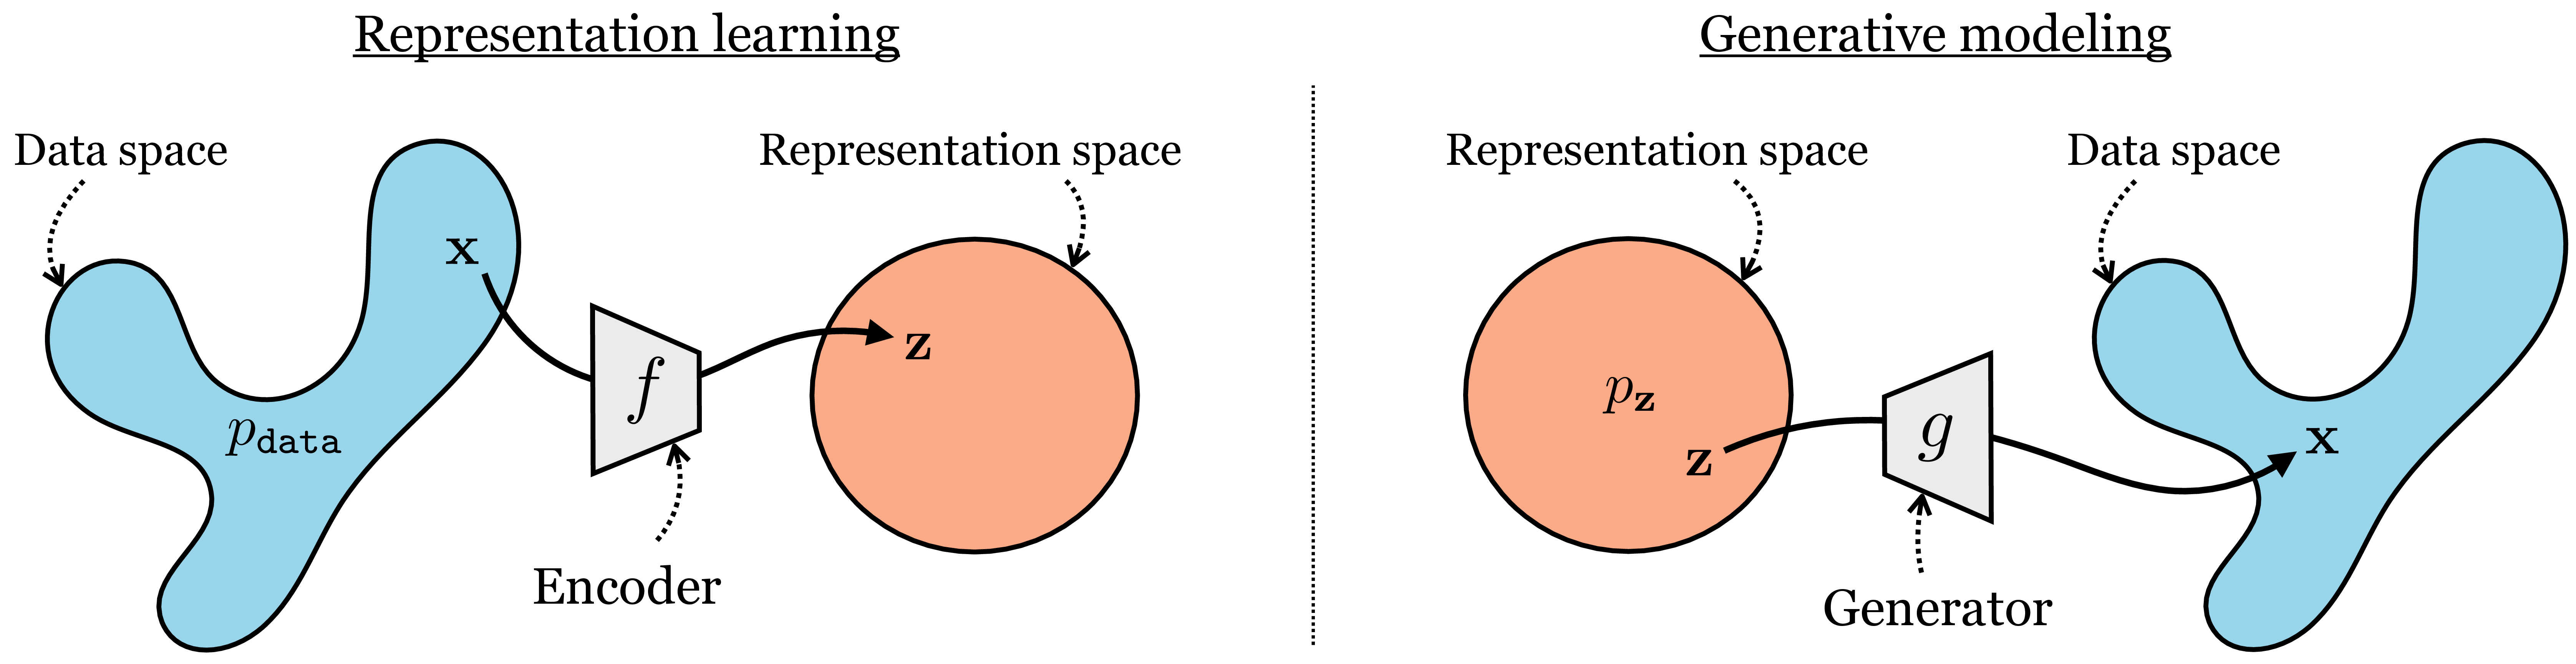
\includegraphics[width=\linewidth]{figures/01_generative_vs_recoding.png}
  \caption{The two complementary directions: representation learning maps observations
  into a useful latent code, whereas generative modelling maps latent variables into the
  data space.}
\end{figure}

\subsection{Generative Framework}

In the generative framework, the world is modeled as a stochastic process:
latent (hidden) sources $\uvec$ are drawn from a source distribution $p_{\uvec}$,
passed through a world model $g(\uvec;\wvec)$, and produce observations $\xvec$.
The learned model distribution $p(\xvec;\wvec)$ must match the observed distribution $p(\xvec)$.

\begin{thmbox}[title={Generative Model Objective}]
Find parameters $\wvec$ such that the model distribution
\[
  p(\xvec;\wvec) = \int_U p_{\uvec}(\uvec)\,\delta\!\bigl(\xvec-g(\uvec;\wvec)\bigr)\dd\uvec
\]
is as close as possible to the empirical distribution $p(\xvec)$.
The loss function measures the distance between these two distributions; typically this
is minimized via \emph{maximum likelihood}.
\end{thmbox}

Key examples of generative models: factor analysis, latent variable models,
Boltzmann machines, hidden Markov models.

\subsection{Recoding Framework}

In the recoding (descriptive) framework, a model $g(\xvec;\wvec)$ maps observations
$\xvec \sim p(\xvec)$ to projections $\uvec$.
The resulting distribution $p(\uvec;\wvec)$ should match a desired \emph{target}
distribution $p_t(\uvec)$:

\begin{itemize}
  \item \textbf{PCA:} projects to a low-dimensional space with maximal retained variance.
        This can be interpreted as maximal information preservation only under additional
        assumptions, for example Gaussian data or isotropic Gaussian reconstruction noise.
        The component directions are orthogonal and their scores are uncorrelated.

  \item \textbf{ICA:} projects into a space with statistically \emph{independent}
        components (factorial code). Algorithms approximate independence by minimising
        mutual information, maximising non-Gaussianity, or maximising likelihood under a
        chosen source distribution. Merely maximising the entropy of a fixed-variance
        linear projection would instead favour a Gaussian and is not the ICA objective.

  \item \textbf{Projection Pursuit:} projects such that components are maximally
        non-Gaussian (since Gaussian components arise from random projections of any
        distribution, by the CLT; non-Gaussian components are informative).
\end{itemize}

\subsection{Recoding and Generative Framework Unified}

Both frameworks can be seen as two sides of the same coin.
In the generative direction: sources $\uvec \xrightarrow{g(\uvec;\wvec)} \xvec$
(sources produce observations).
In the recoding direction: observations $\xvec \xrightarrow{g^{-1}(\xvec;\wvec)} \uvec$
(observations are encoded into sources).
When $g$ is invertible, the change-of-variables formula lets us express the same model
in either direction. That does \emph{not} make arbitrary encoder and decoder objectives
equivalent: the source density, Jacobian term, and loss must match. Under the standard
invertible ICA assumptions, however, INFOMAX and maximum likelihood lead to equivalent
learning rules.


\section{Quality of Parameter Estimation}
\label{sec:quality-estimation}

Generative models must estimate true (but unknown) model parameters.
Let the training data be $\{\xvec\} = \{\xvec^1,\ldots,\xvec^l\}$, collected into the
matrix $\Xmat = (\xvec^1,\ldots,\xvec^l)\T \in \R^{l \times d}$.
The true (unknown) parameter vector is $\wvec$; an estimator maps the data to $\what$.

\begin{defbox}[title={Estimator Quality Measures}]
\begin{align*}
  \text{Unbiased:} \quad & \E_{\Xmat}[\what] = \wvec \\[4pt]
  \text{Bias:} \quad & \bias(\what) = \E_{\Xmat}[\what] - \wvec \\[4pt]
  \text{Variance:} \quad & \Var(\what) = \E_{\Xmat}\!\left[(\what - \E_{\Xmat}[\what])\T(\what - \E_{\Xmat}[\what])\right] \\[4pt]
  \text{MSE:} \quad & \mse(\what) = \E_{\Xmat}\!\left[(\what - \wvec)\T(\what - \wvec)\right]
\end{align*}
\end{defbox}

The fundamental bias-variance decomposition of the MSE is:

\begin{thmbox}[title={Bias-Variance Decomposition}]
\[
  \mse(\what) = \Var(\what) + \bias^2(\what)
\]
\emph{Derivation sketch:} Write $\what - \wvec = (\what - \E[\what]) + (\E[\what] - \wvec)$,
expand the squared norm, and note that the cross-term vanishes because
$\E_{\Xmat}[(\what - \E[\what])(\E[\what] - \wvec)\T] = 0$
(since $\E[\what] - \wvec$ is a constant w.r.t.\ the expectation).
\end{thmbox}

The objective is to minimize the MSE.
Note: the MSE in the parameter estimation sense (expected squared distance to true
parameter) is different from the supervised regression loss (expected squared distance
to true output).

\begin{intbox}
  Unbiasedness and consistency are different properties.
  An \emph{unbiased} estimator has $\E[\what] = \wvec$ for \emph{any} dataset size.
  A \emph{consistent} estimator satisfies $\what \to \wvec$ as $l \to \infty$ ---
  its variance shrinks with more data, but it may be biased for finite $l$.
\end{intbox}

The two properties are genuinely independent, and the classic exam move is to
hand you an estimator that has one but not the other.
Take $\frac{1}{l+1}\sum_{i=1}^{l} X_i$ as an estimator of the mean: its
expectation is $\frac{l}{l+1}\mu \neq \mu$, so it is \emph{biased} --- but the
bias and the variance both die off as $l\to\infty$, so it is \emph{consistent}.
Now take $X_1$, the first sample, as an estimator of the mean: $\E[X_1]=\mu$
makes it \emph{unbiased}, but it never gets better no matter how much data
arrives, so it is \emph{not consistent}.
Bias is about being centred on the truth; consistency is about eventually
collapsing onto it.

\subsection{How good can an estimator possibly get?}

Suppose we restrict ourselves to unbiased estimators.
Is there a floor on how small the variance can be, or can a clever enough
estimator squeeze it arbitrarily close to zero?
There is a floor, and it is set by how sharply the likelihood reacts to the
parameter.
If tweaking $\wvec$ barely changes the probability of the data, the data barely
constrains $\wvec$ and any estimator will be shaky; if a small tweak in $\wvec$
sends the likelihood plummeting, the data pins the parameter down tightly.
The quantity measuring this sensitivity is the \textbf{Fisher information}.

\begin{defbox}[title={Fisher Information (scalar parameter)}]
For a scalar parameter $w$, the Fisher information carried by one observation is the
variance of the score (the derivative of the log-likelihood):
\[
  \mathcal{I}(w)
  = \E\!\left[\left(\pd{}{w}\ln p(\xvec;w)\right)^{\!2}\right]
  = -\,\E\!\left[\pdd{}{w}\ln p(\xvec;w)\right].
\]
It measures the \emph{curvature} of the log-likelihood at its peak: a sharp,
narrow peak means high information.
For $l$ iid samples the information simply adds up: $\mathcal{I}_l(w) = l\,\mathcal{I}(w)$.
For a parameter vector the corresponding object is the Fisher information \emph{matrix},
the expected outer product of score vectors.
\end{defbox}

\begin{thmbox}[title={Cram\'{e}r--Rao Lower Bound}]
Under the usual differentiability and support regularity conditions, any unbiased
estimator $\hat w$ of a scalar parameter satisfies
\[
  \Var(\hat w) \;\geq\; \frac{1}{\mathcal{I}_l(w)}.
\]
The variance of the estimator is bounded below by the \emph{inverse} of the
Fisher information.
An estimator that attains this bound --- the smallest variance physically
available --- is called \textbf{efficient}.
\end{thmbox}

\begin{notebox}[title={Exam trap: which quantity does Cram\'{e}r--Rao bound?}]
The Cram\'{e}r--Rao bound relates the \textbf{variance} of $\what$ to the inverse
Fisher information --- not the bias, not the expected value, not the MSE.
And an estimator reaching the bound is \textbf{efficient}, not ``consistent''
or ``unbiased'' (unbiasedness is a \emph{precondition} for the bound, not its
conclusion).
These three words --- consistent, efficient, unbiased --- get shuffled around in
exam questions constantly; keep them straight:
\emph{unbiased} = centred correctly,
\emph{consistent} = converges with more data,
\emph{efficient} = has the smallest variance the bound allows.
\end{notebox}


\section{Information Theory Essentials}
\label{sec:info-theory}

Information theory connects many objectives in this course, but not always in the same
way. ICA can minimise mutual information and $t$-SNE explicitly minimises a KL
divergence. Maximum likelihood --- used by EM and Boltzmann machines --- is equivalent
to minimising the forward KL divergence from the empirical data distribution to the
model, up to a constant. NMF only has a KL interpretation for its KL-divergence loss;
the common squared-error version does not. PCA's retained variance has an information
interpretation only under suitable probabilistic assumptions.
So it pays to get the vocabulary straight once, here, rather than re-deriving it
in every chapter.

\begin{defbox}[title={Entropy, Joint \& Conditional Entropy, Mutual Information}]
For a discrete random variable $X$ with distribution $p(x)$:
\[
  H(X) = -\sum_{x} p(x)\log p(x),
  \qquad\text{with the convention } 0\cdot\log 0 = 0.
\]
For a pair $(X,Y)$ with joint distribution $p(x,y)$:
\[
  H(X,Y) = -\sum_{x,y} p(x,y)\log p(x,y),
  \qquad
  H(X\mid Y) = H(X,Y) - H(Y).
\]
The \textbf{mutual information} is the information the two variables share:
\[
  \MI(X;Y)
  = \sum_{x,y} p(x,y)\,\log\frac{p(x,y)}{p(x)\,p(y)}
  = H(X) + H(Y) - H(X,Y).
\]
$\MI(X;Y)\geq 0$, with equality \emph{iff} $X$ and $Y$ are independent.
\end{defbox}

Entropy is ``how surprised am I, on average, by a draw from this distribution''.
It is zero for a deterministic variable (no surprise ever) and maximal for the
uniform distribution (every outcome equally unexpected).
Mutual information is then ``how much does knowing $Y$ reduce my surprise about
$X$'' --- which is why it is exactly zero when the two are independent, and why
ICA hunts for the projection that drives it to zero.

\begin{notebox}[title={Entropy is not bounded by 1}]
A perennial exam distractor claims ``the entropy of a probability distribution
is always $\geq 0$ and $\leq 1$''.
The lower bound is right, the upper bound is nonsense: a uniform distribution
over $k$ outcomes has entropy $\log k$, which grows without limit.
(With $\log_2$ you get $1$ bit for a fair coin --- probably the source of the
confusion --- but even then three equally likely outcomes already give
$\log_2 3 \approx 1.58$.)
Watch the base of the logarithm too: exams here usually ask for the
\emph{natural} logarithm, so a fair coin gives $\ln 2 \approx 0.69$, not $1$.
\end{notebox}

\begin{exbox}[title={Computing marginals, entropies, and mutual information}]
Given the joint distribution of two binary variables:
\[
\begin{array}{c|cc}
 & Y=0 & Y=1\\
\hline
X=0 & 0.3 & 0.4\\
X=1 & 0.2 & 0.1
\end{array}
\]
\textbf{Marginals} are row and column sums:
$p(X{=}0)=0.3+0.4=0.7$ and $p(Y{=}0)=0.3+0.2=0.5$.

\textbf{Entropies} (natural log) come from the marginals only:
\[
  H(X) = -(0.7\ln 0.7 + 0.3\ln 0.3) \approx 0.61,
  \qquad
  H(Y) = -(0.5\ln 0.5 + 0.5\ln 0.5) = \ln 2 \approx 0.69.
\]
\textbf{Joint entropy} uses all four cells:
\[
  H(X,Y) = -(0.3\ln 0.3 + 0.4\ln 0.4 + 0.2\ln 0.2 + 0.1\ln 0.1) \approx 1.28.
\]
\textbf{Mutual information} is then the leftover:
\[
  \MI(X;Y) = H(X) + H(Y) - H(X,Y) \approx 0.61 + 0.69 - 1.28 = 0.02.
\]
The tiny value says these two variables are \emph{almost} independent --- if they
were exactly independent, every cell would equal the product of its margins
($0.7\times0.5=0.35 \neq 0.3$), and $\MI$ would be exactly $0$.
\end{exbox}

Finally, the workhorse of the whole course: a way to measure how far one
distribution is from another.

\begin{defbox}[title={Kullback--Leibler Divergence}]
For distributions $p$ and $q$ over the same space:
\[
  \KL{p}{q} = \sum_{x} p(x)\,\log\frac{p(x)}{q(x)}
  \qquad\text{(discrete)},
  \qquad
  \KL{p}{q} = \int p(x)\,\log\frac{p(x)}{q(x)}\dd x
  \qquad\text{(continuous)}.
\]
Properties:
\begin{itemize}
  \item $\KL{p}{q} \geq 0$, with equality \emph{iff} $p = q$ (Gibbs' inequality).
  \item It is \textbf{not symmetric}: $\KL{p}{q} \neq \KL{q}{p}$ in general ---
        it is a divergence, not a distance (and it violates the triangle inequality).
  \item It is infinite if $q(x) = 0$ somewhere that $p(x) > 0$: $p$'s support must
        sit inside $q$'s support.
  \item Mutual information is a special case:
        $\MI(X;Y) = \KL{p(x,y)}{p(x)p(y)}$ --- the divergence between the true
        joint and the joint you would get if the variables were independent.
\end{itemize}
\end{defbox}

\begin{exbox}[title={Two KL computations you should be able to do cold}]
\textbf{Discrete.} With $p=(0.8,\,0.2)$ and $q=(0.5,\,0.5)$:
\[
  \KL{p}{q}
  = 0.8\ln\frac{0.8}{0.5} + 0.2\ln\frac{0.2}{0.5}
  = 0.8(0.470) + 0.2(-0.916)
  \approx 0.19.
\]
\textbf{Continuous (two uniforms).} Let $p_Y$ be uniform on $[0,\theta_Y]$ and
$p_Z$ uniform on $[0,\theta_Z]$, with $\theta_Y \leq \theta_Z$.
The integrand is nonzero only where $p_Y>0$, and there the density ratio is the
constant $\theta_Z/\theta_Y$, so the integral collapses:
\[
  \KL{p_Y}{p_Z}
  = \int_0^{\theta_Y}\frac{1}{\theta_Y}\,\ln\frac{1/\theta_Y}{1/\theta_Z}\dd x
  = \ln\frac{\theta_Z}{\theta_Y}.
\]
With $\theta_Y=e^{5}$ and $\theta_Z=e^{10}$ this is just $10-5=5$.
Note the asymmetry biting: $\KL{p_Z}{p_Y}$ would be \emph{infinite}, because
$p_Z$ puts mass where $p_Y$ is zero.
\end{exbox}


\section{Maximum Likelihood Estimator}
\label{sec:mle}

\begin{defbox}[title={Likelihood}]
The \textbf{likelihood} of the dataset $\{\xvec\} = \{\xvec^1,\ldots,\xvec^l\}$ under
model parameters $\wvec$ is
\[
  \lhood(\{\xvec\};\wvec) \;=\; p(\{\xvec\};\wvec),
\]
the probability that the model $p(\xvec;\wvec)$ produces the observed data.
For \textbf{iid} (independent, identically distributed) data this factorizes:
\[
  \lhood(\{\xvec\};\wvec) \;=\; \prod_{i=1}^{l} p(\xvec^i;\wvec).
\]
Working in log-space converts the product to a sum (negative log-likelihood, NLL):
\[
  -\ln \lhood(\{\xvec\};\wvec) \;=\; -\sum_{i=1}^{l} \ln p(\xvec^i;\wvec).
\]
\end{defbox}

Maximum likelihood estimation (MLE) is the dominant objective in unsupervised learning.
It finds the parameters $\wvec$ that make the observed data most probable under the model:
\[
  \what_{\mathrm{ML}} = \argmax_{\wvec} \lhood(\{\xvec\};\wvec) = \argmin_{\wvec} \bigl[-\ln\lhood(\{\xvec\};\wvec)\bigr].
\]

\begin{thmbox}[title={Properties of the MLE}]
Under standard regularity conditions and when the model is identifiable and correctly
specified, the maximum likelihood estimator is:
\begin{itemize}
  \item \textbf{Invariant under reparameterization:} if $\hat{\wvec}$ is the MLE of
        $\wvec$, then $f(\hat{\wvec})$ is an MLE of $f(\wvec)$, with the usual care
        needed for non-injective transformations.
  \item \textbf{Asymptotically unbiased and efficient:} for large $l$, the MLE achieves
        the Cram\'{e}r-Rao lower bound, i.e.\ it has the smallest possible variance among
        all unbiased estimators. It is asymptotically optimal.
  \item \textbf{Asymptotically consistent:} $\what \to \wvec$ as $l \to \infty$.
\end{itemize}
\end{thmbox}

\begin{notebox}[title={MLE caveats}]
MLE can overfit for small datasets (it uses no prior information).
For finite $l$, MLE may be biased: the classic example is the MLE of the variance of a
Gaussian, $\hat{\sigma}^2 = \frac{1}{l}\sum(x_i - \bar{x})^2$, which underestimates
the true variance (the unbiased estimator uses $l-1$).
\end{notebox}


\section{Expectation Maximization}
\label{sec:em}

Many generative models include \emph{latent (hidden) variables} $\uvec$ that are not
directly observed.
The marginal likelihood then requires integrating over all latent configurations:
\[
  p(\xvec;\wvec) = \int_U p_{\uvec}(\uvec)\,\delta\!\bigl(\xvec-g(\uvec;\wvec)\bigr)\dd\uvec.
\]
This integral is in general intractable due to:
\begin{itemize}
  \item hidden states (discrete or continuous latent variables),
  \item many-to-one output mappings ($g$ is not injective),
  \item non-linearities in $g$.
\end{itemize}

The \textbf{Expectation Maximization (EM)} algorithm circumvents this by working with
the \emph{joint} distribution $p(\xvec, \uvec;\wvec)$, which is easier to handle, and
by constructing a tractable lower bound on the log-likelihood.

\paragraph{Derivation of the lower bound}
Introduce an arbitrary distribution $Q(\uvec \given \{\xvec\})$ over latent variables.
Apply Jensen's inequality to the concave logarithm:
\begin{align*}
  \ln \lhood(\{\xvec\};\wvec)
  &= \ln \int_U p(\{\xvec\},\uvec;\wvec)\,\dd\uvec \\
  &= \ln \int_U Q(\uvec \given \{\xvec\})\,
     \frac{p(\{\xvec\},\uvec;\wvec)}{Q(\uvec \given \{\xvec\})}\,\dd\uvec \\
  &\geq \int_U Q(\uvec \given \{\xvec\})\,
     \ln\frac{p(\{\xvec\},\uvec;\wvec)}{Q(\uvec \given \{\xvec\})}\,\dd\uvec
  \;\eqdef\; \Fbound(Q,\wvec).
\end{align*}
$\Fbound(Q,\wvec)$ is the \textbf{free energy} (ELBO: evidence lower bound).
Equivalently, the bound can be rewritten as
\[
  \Fbound(Q,\wvec)
  = \ln\lhood(\{\xvec\};\wvec)
    - \KL{Q(\uvec\given\{\xvec\})}{p(\uvec\given\{\xvec\};\wvec)},
\]
which makes the E-step obvious: to maximize $\Fbound$ over $Q$ (with $\wvec$ fixed)
one minimizes the KL divergence, which is zero iff $Q = p(\uvec\given\{\xvec\};\wvec)$.

\begin{thmbox}[title={EM Algorithm}]
EM alternates between two steps until convergence:
\begin{align*}
  \textbf{E-step:} \quad & Q_{k+1} = \argmax_{Q}\; \Fbound(Q,\wvec_k)
    \quad \Rightarrow \quad Q_{k+1} = p(\uvec \given \{\xvec\};\wvec_k) \\[4pt]
  \textbf{M-step:} \quad & \wvec_{k+1} = \argmax_{\wvec}\; \Fbound(Q_{k+1},\wvec)
\end{align*}
\end{thmbox}

\begin{figure}[H]
  \centering
  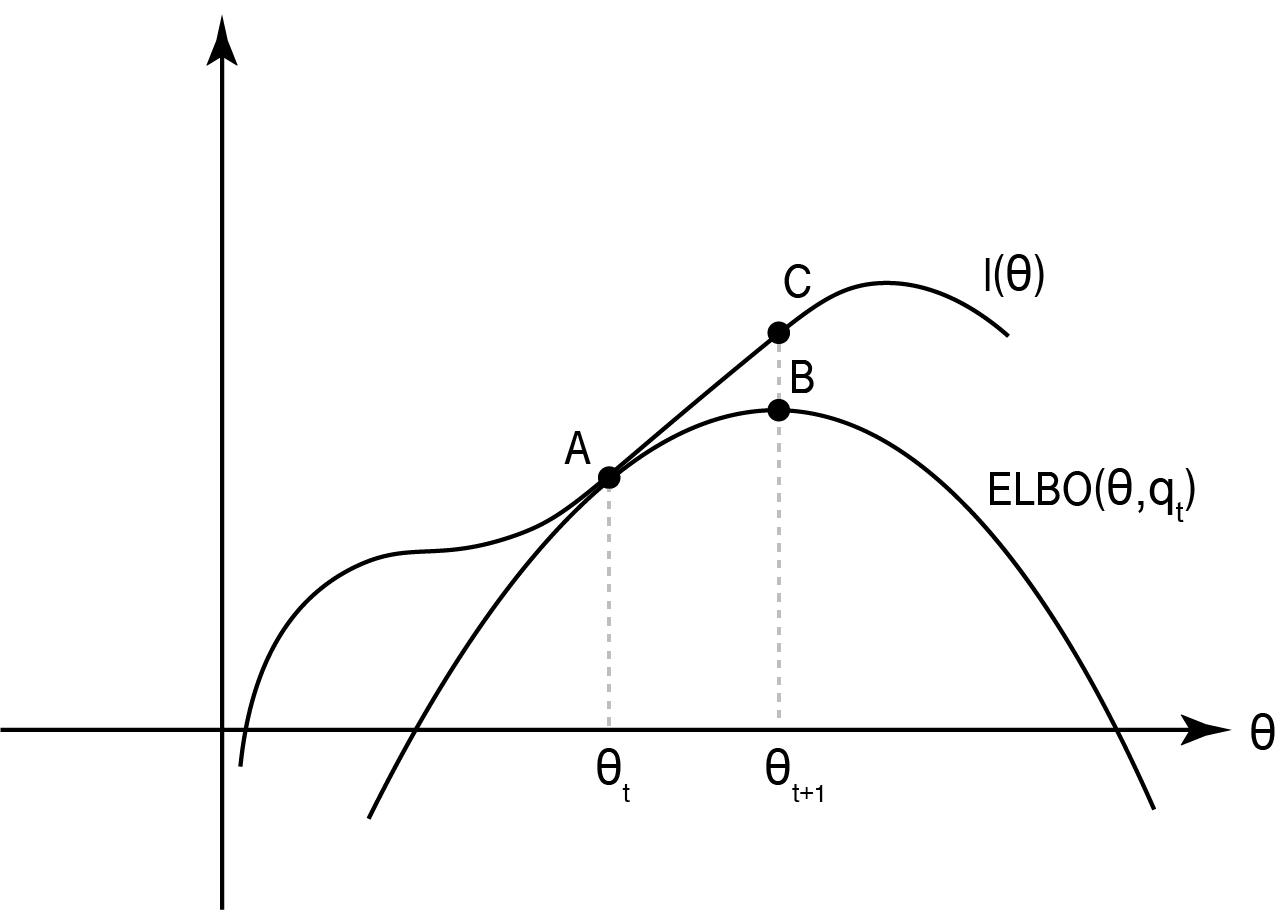
\includegraphics[width=.72\linewidth]{figures/02_em_elbo_coordinate_ascent.png}
  \caption{EM viewed as coordinate ascent. The E-step makes the ELBO touch the
  log-likelihood at the current parameters; the M-step moves to a parameter value with
  a higher bound and therefore a non-decreased likelihood.}
\end{figure}

\paragraph{Monotone convergence}
Both steps can only increase (or leave unchanged) the lower bound $\Fbound$.
The E-step tightens the bound: at the beginning of the M-step,
$\Fbound(Q_{k+1},\wvec_k) = \ln\lhood(\{\xvec\};\wvec_k)$ (the bound is tight).
The M-step then increases $\Fbound$, which implies:
\[
  \ln\lhood(\{\xvec\};\wvec_k) \;\leq\; \Fbound(Q_{k+1},\wvec_{k+1}) \;\leq\; \ln\lhood(\{\xvec\};\wvec_{k+1}).
\]
Therefore the log-likelihood is guaranteed to be non-decreasing at every EM iteration.

\begin{intbox}
  The E-step does not change model parameters --- it only updates the posterior
  distribution over latent variables. The M-step maximizes the expected complete-data
  log-likelihood, which for exponential family models has a closed-form solution.
  EM converges to a stationary point (often a local maximum, but possibly a saddle point
  or boundary solution), not necessarily to the global optimum.
\end{intbox}

EM is applied throughout this course: Baum-Welch algorithm for HMMs, fitting Gaussian
mixtures, factor analysis, and (soft) ICA variants.


\section{Maximum Entropy}
\label{sec:maxent}

Suppose you know a few facts about a distribution --- its mean, maybe its
variance --- but nothing else, and you have to commit to a full distribution
anyway.
Which one do you pick?
Picking any particular shape smuggles in assumptions you cannot justify.
The maximum entropy principle says: pick the \emph{least committal} distribution
that still respects the facts you actually have.
Since entropy measures uncertainty (\cref{sec:info-theory}), the most uncertain
distribution consistent with your constraints is the one that assumes the least
beyond them.

\begin{defbox}[title={Principle of Maximum Entropy}]
Among all distributions consistent with the available constraints (e.g.\ known
moments), choose the one with \emph{maximum entropy}
$H = -\sum_{k\ge1} p_k\log p_k$.
\end{defbox}

This distribution:
\begin{itemize}
  \item makes the minimal assumptions beyond the stated constraints,
  \item corresponds to the most likely empirical distribution that could give rise to the
        observed features,
  \item connects statistical mechanics (thermodynamic equilibrium) and information theory.
\end{itemize}

\begin{notebox}[title={Existence caveat}]
Not every class of distributions contains a maximum entropy member.
For example, the class of all distributions with a given mean has arbitrarily large
entropy (entropy can be pushed to $\infty$).
The class of distributions with mean zero, second moment one, and third moment one has
entropy bounded from above but the supremum is not attained.
\end{notebox}

\paragraph{Maximum entropy with moment constraints}
Given moment constraints $\sum_{i=1}^n p(x_i)\,f_k(x_i) = F_k$ for $k=1,\ldots,m$
and normalization $\sum_{i=1}^n p(x_i) = 1$, the maximum entropy solution is the
\textbf{Gibbs distribution}:

\begin{thmbox}[title={Gibbs Distribution (MaxEnt Solution)}]
\[
  p(x_i) = \frac{1}{Z(\lambda_1,\ldots,\lambda_m)}
  \exp\!\bigl(\lambda_1 f_1(x_i) + \cdots + \lambda_m f_m(x_i)\bigr),
\]
with \textbf{partition function}
\[
  Z(\lambda_1,\ldots,\lambda_m) = \sum_{i=1}^n \exp\!\bigl(\lambda_1 f_1(x_i) + \cdots + \lambda_m f_m(x_i)\bigr).
\]
The Lagrange multipliers $\lambda_k$ are determined by the constraint equations:
\[
  F_k = \pd{}{\lambda_k} \log Z(\lambda_1,\ldots,\lambda_m), \qquad k = 1,\ldots,m.
\]
\end{thmbox}

\begin{exbox}[title={Standard MaxEnt examples}]
\begin{itemize}
  \item \textbf{Normal distribution:} maximum entropy distribution given fixed mean and
        variance. Constraints: $\E[X] = \mu$ and $\E[X^2] = \mu^2 + \sigma^2$.
  \item \textbf{Uniform distribution:} maximum entropy on a bounded interval $[a,b]$.
        Only constraint: support.
  \item \textbf{Exponential distribution:} maximum entropy on $[0,\infty)$ given fixed mean.
        Constraint: $\E[X] = 1/\lambda$.
\end{itemize}
\end{exbox}

\begin{intbox}
  The MaxEnt principle explains one precise reason Gaussian models appear so frequently:
  among all continuous distributions with a \emph{fixed mean and variance}, the Gaussian
  has maximum differential entropy. Finite variance by itself does not make a process
  Gaussian, and an energy constraint does not guarantee convergence to a Gaussian.
  In ICA, maximizing entropy of a nonlinear transform of the data is equivalent to
  maximizing likelihood of an independent-component model (INFOMAX).
\end{intbox}


% ==========================================================
\chapter{Principal Component Analysis}
% ==========================================================

\section{The Method}

PCA answers a simple question: if the data really lives in fewer dimensions than we
measured, which few directions capture most of what is going on? It rotates the data
onto a new set of orthogonal axes --- the \emph{principal directions} --- ordered so that
the first captures the most variance, the second the most of what is left, and so on.
Keep the top few and you have a faithful low-dimensional picture of the data; the rest is
mostly noise or redundancy you can throw away. Everything below is just the linear algebra
that makes this precise.

Let the data matrix be $\bm{X} \in \R^{n \times m}$, where $n$ is the number of samples
and $m$ is the number of features (the rows $\bm{x}_i \in \R^m$ are centered so that
$\sum_i \bm{x}_i = \bm{0}$).

The \textbf{sample covariance matrix} is
\[
  \bm{C} = \frac{1}{n}\bm{X}\T\bm{X} \in \R^{m \times m}.
\]
Its eigendecomposition $\bm{C} = \bm{U}\bm{\Lambda}\bm{U}\T$ yields an orthogonal
matrix $\bm{U}$ whose columns $\bm{u}_k$ are the principal directions (\emph{loadings}),
and a diagonal matrix $\bm{\Lambda} = \mathrm{diag}(\lambda_1,\ldots,\lambda_m)$ of
eigenvalues sorted in decreasing order.

The \textbf{SVD} of $\bm{X}$ gives the same result: $\bm{X} = \bm{V}\bm{D}\bm{U}\T$
with $\bm{V} \in \R^{n \times n}$, $\bm{D} \in \R^{n \times m}$ diagonal, and
$\bm{U} \in \R^{m \times m}$ orthogonal.
The eigenvalues of $\bm{C}$ are $\lambda_k = d_k^2/n$ where $d_k$ are the singular values.

\begin{defbox}[title={PCA Projection}]
The \textbf{principal component scores} (projections) are collected in
\[
  \bm{Y} = \bm{X}\bm{U} = \bm{V}\bm{D} \in \R^{n \times m}.
\]
The $k$-th column $\bm{y}_k = \bm{X}\bm{u}_k$ is the projection of all data points
onto the $k$-th principal direction.
The original data can be reconstructed as the outer product sum
\[
  \bm{X} = \sum_{k=1}^{m} \bm{y}_k \bm{u}_k\T.
\]
\end{defbox}

\figureplaceholder
  {Geometric view of PCA and low-rank reconstruction.}
  {A centred two-dimensional point cloud with its covariance ellipse, PC1 along the long axis and PC2 along the short axis. Project points onto PC1 and draw the perpendicular reconstruction residuals.}
  {PCA geometric interpretation covariance ellipse projection reconstruction error}

\paragraph{Online learning: Oja's rule}
A single-component PCA can be learned online (one sample at a time) using
\textbf{Oja's rule}:
\[
  \bm{u}^{\mathrm{new}} = \bm{u} + \eta\bigl(t\,\bm{x} - t^2\,\bm{u}\bigr),
  \qquad t = \bm{u}\T\bm{x}.
\]
This is a fixed-point iteration analogous to the power method.


\section{Variance Maximization}

PCA can be motivated as the projection that maximizes the variance of the projected data.

The first principal direction solves
\[
  \bm{u}_1 = \argmax_{\|\bm{u}\|=1} \frac{1}{n}\sum_{i=1}^{n}(\bm{u}\T\bm{x}_i)^2
  = \argmax_{\|\bm{u}\|=1} \bm{u}\T\bm{C}\bm{u}.
\]

\begin{thmbox}[title={Variance Maximization Solution}]
Using the eigendecomposition $\bm{C} = \sum_k \lambda_k \bm{u}_k\bm{u}_k\T$ and writing
$\bm{u} = \sum_k a_k \bm{u}_k$, the objective becomes
$\bm{u}\T\bm{C}\bm{u} = \sum_k a_k^2 \lambda_k$ subject to $\sum_k a_k^2 = 1$.
This is maximized by $a_1 = 1$, all others zero:
\[
  \bm{u}_1 = \text{eigenvector of } \bm{C} \text{ with largest eigenvalue } \lambda_1.
\]
The $k$-th principal direction is the direction of maximal variance \emph{orthogonal} to
all previous $k-1$ directions.
The variance explained by the $k$-th component equals $\lambda_k$.
\end{thmbox}

\begin{intbox}[title={Why eigenvectors, of all things?}]
The algebra above is short enough to hide what actually happened, so here it is in
words.
Writing $\bm{u} = \sum_k a_k\bm{u}_k$ expresses the candidate direction in the
eigenvector basis, and the objective becomes $\sum_k a_k^2\lambda_k$ with the
budget $\sum_k a_k^2 = 1$.
That is now a completely transparent problem: you have one unit of ``weight'' to
distribute, each eigenvector pays you its eigenvalue per unit, so obviously you
dump the entire budget on the highest-paying one.
The maximum-variance direction \emph{is} the top eigenvector, not by coincidence
but because the eigendecomposition already sorted the directions by exactly the
quantity you are maximising.

Geometrically: the covariance matrix stretches space, most along its top
eigenvector.
PCA just asks ``which way is the data cloud longest?'', and the answer to that
question is what an eigendecomposition computes.
\end{intbox}

\begin{notebox}[title={Exam trap: singular values are not eigenvalues}]
The singular values $d_k$ of the data matrix $\bm{X}$ and the eigenvalues
$\lambda_k$ of $\bm{X}\T\bm{X}$ are related by a \emph{square root}, not equality:
\[
  d_k = \sqrt{\lambda_k}
  \qquad\text{(equivalently } \lambda_k = d_k^2\text{, or } d_k^2/n \text{ for the
  covariance matrix }\bm{C}\text{).}
\]
``The singular values of $\bm{X}$ equal the eigenvalues of $\bm{X}\T\bm{X}$'' is a
recurring distractor --- it is off by exactly that square root.

While we are here, two more that get recycled: the matrix of eigenvectors $\bm{U}$
is \textbf{orthogonal}, not symmetric; and the eigenvalues of $\bm{X}\T\bm{X}$ are
non-negative and sum to the \emph{total variance}, not to $1$.
\end{notebox}


\section{Uniqueness}

PCA is \textbf{unique up to sign flips} of the principal directions, provided all
eigenvalues are distinct.
If two or more eigenvalues are equal (degenerate case), the corresponding eigenvectors
span a subspace but their individual directions are arbitrary; any orthonormal basis
of that subspace is equally valid.

\begin{notebox}[title={Zero eigenvalues}]
Zero eigenvalues mean the data lies in a lower-dimensional affine subspace (rank-deficient
covariance matrix). There can be \emph{many} zero eigenvalues: if the data of dimension
$m$ spans only a $k$-dimensional subspace, then $m - k$ eigenvalues are zero.
The corresponding principal directions can be discarded without any loss.
\end{notebox}


\section{Properties of PCA}
\label{sec:pca-properties}

Let $\bm{y}^{(i)} = \bm{U}\T\bm{x}_i$ be the projection of sample $i$.

\begin{thmbox}[title={Key Properties of PCA Projections}]
\begin{itemize}
  \item \textbf{Zero mean:} $\sum_i y_k^{(i)} = 0$ for all $k$ (because the data are centered).
  \item \textbf{Uncorrelated:} $\mathrm{Cov}(y_k, y_l) = 0$ for $k \neq l$
        (follows from orthogonality of $\bm{U}$).
  \item \textbf{Variance:} $\mathrm{Var}(y_k) = \lambda_k$ (the $k$-th eigenvalue).
  \item \textbf{Optimal reconstruction:} truncating to the first $l$ components gives
        the best rank-$l$ approximation in terms of MSE:
        \[
          \mathrm{MSE}_l = \sum_{k=l+1}^{m} \lambda_k.
        \]
  \item \textbf{Fraction of variance} explained by the first $l$ components:
        $\frac{\sum_{k=1}^l \lambda_k}{\sum_{k=1}^m \lambda_k}$.
\end{itemize}
\end{thmbox}

\paragraph{Derivation of the MSE formula}
Retain the first $l$ components.
The reconstruction of sample $\bm{x}_i$ is
$\hat{\bm{x}}_i = \sum_{k=1}^l (\bm{u}_k\T\bm{x}_i)\bm{u}_k$,
so the residual is
$\bm{x}_i - \hat{\bm{x}}_i = \sum_{k=l+1}^m (\bm{u}_k\T\bm{x}_i)\bm{u}_k$.
By orthonormality of the $\bm{u}_k$:
\[
  \|\bm{x}_i - \hat{\bm{x}}_i\|^2 = \sum_{k=l+1}^m \bigl(\bm{u}_k\T\bm{x}_i\bigr)^2.
\]
Averaging over all $n$ samples and using
$\frac{1}{n}\sum_{i=1}^n (\bm{u}_k\T\bm{x}_i)^2 = \bm{u}_k\T\bm{C}\bm{u}_k = \lambda_k$:
\[
  \mathrm{MSE}_l
  = \frac{1}{n}\sum_{i=1}^n \|\bm{x}_i - \hat{\bm{x}}_i\|^2
  = \sum_{k=l+1}^m \bm{u}_k\T\bm{C}\bm{u}_k
  = \sum_{k=l+1}^m \lambda_k.
\]
Any other rank-$l$ projection gives a larger MSE, so the top $l$ eigenvectors are
the optimal choice.


\section{Examples}

\subsection{Iris Data Set}

The Iris dataset has $n = 150$ samples (50 per species: \textit{setosa}, \textit{versicolor},
\textit{virginica}) and $m = 4$ features (sepal length, sepal width, petal length, petal width).

PC1 accounts for approximately \textbf{92\% of the variance} when the raw features are
centred but not scaled, and clearly separates \textit{setosa} from the other species.
Distinguishing \textit{versicolor} from \textit{virginica} also benefits from PC2;
the exact percentages and plots depend on whether the four features were standardised.
The example illustrates an important warning: a high-variance direction can expose
class structure, but PCA never uses class labels and does not optimise separation.

\subsection{Multiple Tissue Data Set}

This microarray dataset contains expression values for 5{,}565 genes across 102 samples
from four human tissue types: \textbf{breast} (Br), \textbf{prostate} (Pr),
\textbf{lung} (Lu), and \textbf{colon} (Co).

Applied to all genes simultaneously:
\begin{itemize}
  \item PC1 (5\% variance) separates prostate from the rest.
  \item PC2 (3\%) separates colon and also breast samples.
  \item PC3 (3\%) partially separates lung.
\end{itemize}

\paragraph{Variance filtering}
Selecting only the top-variance genes before PCA is justified for microarray data
(most genes are essentially constant noise).
Three filtered subsets were compared:
\begin{itemize}
  \item \textbf{101 genes} (highest variance, XMultiF1): PC1 (36\%) separates prostate;
        PC2 (14\%) separates colon; PC3 (8\%) separates breast and lung.
        Much cleaner separation than the full set.
  \item \textbf{13 genes} (XMultiF2, 57\% PC1): similar tissue-level separation.
  \item \textbf{5 genes} (XMultiF3, 77\% PC1): still separates prostate clearly but
        other tissues become hard to distinguish.
        Inspection reveals 4 of the 5 selected genes are highly correlated (ACPP, KLK2,
        MSMB, TRGC2 --- all prostate-related; KRT5 is not).
\end{itemize}

\paragraph{Gene clustering}
Applying hierarchical clustering with correlation as distance metric, then selecting the
gene with maximal variance per cluster (\textbf{92 uncorrelated genes of maximal variance})
gives very similar results to variance-based filtering.
The approach ensures genes are not redundant (correlated genes contribute the same
information to PCA) while still selecting high-variance representatives.


\section{Kernel Principal Component Analysis}

\subsection{The Method}

\textbf{Kernel PCA} (KPCA) extends PCA to nonlinear projections by performing the
linear operations of PCA inside a \emph{reproducing kernel Hilbert space} (RKHS), to
which the data are first mapped non-linearly:
\[
  \bm{x} \;\mapsto\; \Phi(\bm{x}).
\]

Assuming the mapped data are centered ($\sum_i \Phi(\bm{x}_i) = \bm{0}$), the
covariance in feature space is
$\bm{C} = \frac{1}{n}\sum_i \Phi(\bm{x}_i)\Phi(\bm{x}_i)\T$,
and the Gram (kernel) matrix has entries $K_{ij} = \Phi(\bm{x}_j)\T\Phi(\bm{x}_i) = k(\bm{x}_i,\bm{x}_j)$.

The eigenvalue problem $\bm{C}\bm{w} = \lambda\bm{w}$ cannot be solved in feature space
directly (we only have $K_{ij}$), but the solution must lie in the span of the mapped
data:
\[
  \bm{w} = \sum_{i=1}^n \alpha_i\,\Phi(\bm{x}_i).
\]
Substituting and using $K_{ij}$ yields the \textbf{kernel eigenvalue problem}:
\[
  n\lambda\,\bm{K}\bm{\alpha} = \bm{K}^2\bm{\alpha}
  \;\;\Rightarrow\;\;
  n\lambda\,\bm{\alpha} = \bm{K}\bm{\alpha}.
\]
Normalization $\|\bm{w}\|=1$ requires $\|\bm{\alpha}\| = 1/\sqrt{\tilde\lambda}$ where
$\tilde\lambda = n\lambda$, so
\[
  \bm{\alpha} = \frac{\tilde{\bm{\alpha}}}{\sqrt{\tilde\lambda}}.
\]

The projection of a new point $\bm{x}$ onto a kernel principal direction is then
\[
  \bm{w}\T\Phi(\bm{x}) = \sum_{i=1}^n \alpha_i\,k(\bm{x}_i,\bm{x}).
\]

\begin{thmbox}[title={Kernel PCA Algorithm}]
\begin{enumerate}
  \item \textbf{Center} the Gram matrix:
        $\tilde{\bm{K}} = \bm{K} - \frac{1}{n}\bm{K}\bm{1}\bm{1}\T - \frac{1}{n}\bm{1}\bm{1}\T\bm{K} + \frac{1}{n^2}(\bm{1}\T\bm{K}\bm{1})\bm{1}\bm{1}\T$.
  \item \textbf{Eigenvalues}: compute eigenvectors $\bm{\alpha}$ and eigenvalues
        $\tilde\lambda$ of $\tilde{\bm{K}}$.
  \item \textbf{Normalize}: $\alpha_i^{\mathrm{new}} = \alpha_i/(\|\bm{\alpha}\|\sqrt{n\lambda})$.
  \item \textbf{Project} a new vector $\bm{x}$: center its kernel vector and compute
        $\bm{w}\T\Phi(\bm{x}) = \sum_i \alpha_i\,k(\bm{x}_i,\bm{x})$.
\end{enumerate}
\end{thmbox}

\begin{figure}[H]
  \centering
  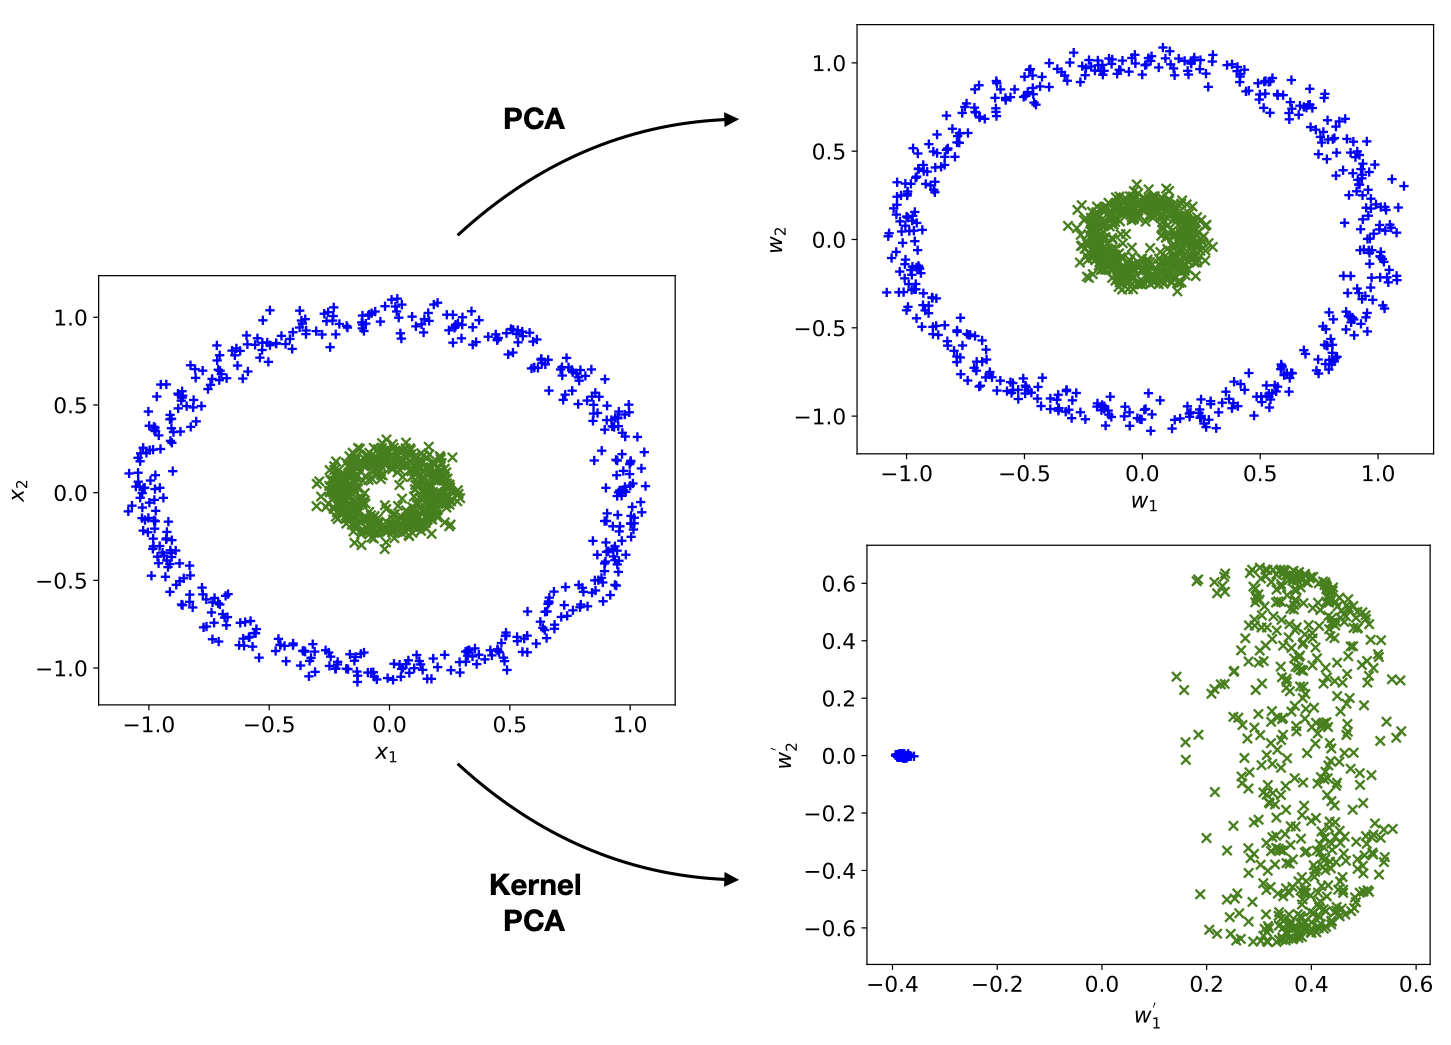
\includegraphics[width=.93\linewidth]{figures/03_kernel_pca_concentric_circles.png}
  \caption{Linear PCA cannot unfold concentric rings, whereas an appropriate kernel
  produces coordinates in which the two groups can be separated.}
\end{figure}

\begin{intbox}
  Kernel PCA can detect nonlinear structure that linear PCA misses.
  For example, concentric rings are linearly inseparable but perfectly separable in
  the RKHS of an RBF kernel.
  The price is that the representation depends on all training points (no compact weight
  vector $\bm{u}$), and choosing the right kernel function requires domain knowledge.
\end{intbox}

The entire trick is that we never touch $\Phi$ itself.
Note what the projection formula
$\bm{w}\T\Phi(\bm{x}) = \sum_i \alpha_i\,k(\bm{x}_i,\bm{x})$
actually needs: only \emph{kernel evaluations}, never the feature vectors.
That is the kernel trick --- the feature space may be enormous, even
infinite-dimensional, and we never pay for it, because everything we want is
expressible through inner products that $k$ computes for us directly.

\begin{notebox}[title={$\bm{K}$ and $\bm{C}$: same rank, different size}]
Two things about the Gram matrix $\bm{K}$ and the feature covariance $\bm{C}$ are
routinely confused.

\textbf{They have different dimensions.}
$\bm{K}$ is $n\times n$ (one row per \emph{data point}), while $\bm{C}$ lives in
feature space and is as big as the feature space itself --- possibly infinite.
This is precisely why we solve the eigenproblem of $\bm{K}$ instead of $\bm{C}$.

\textbf{But they share their nonzero eigenvalues}, and therefore their rank.
So the claim ``$\bm{K}$ and $\bm{C}$ always have the same dimensionality
\emph{and} the same rank'' is a half-truth --- the rank half is right, the
dimensionality half is wrong.

One more caveat worth having straight: centering $\bm{K}$ \emph{is} required, but
not because ``eigenvalues of $\bm{K}$ could be negative''.
$\bm{K}$ is positive semidefinite, so its eigenvalues are never negative.
Centering is required because the PCA derivation assumes the mapped data has zero
mean in feature space, and $\Phi(\bm{x})$ generally does not.
\end{notebox}


% ==========================================================
\chapter{Independent Component Analysis}
% ==========================================================

Two people are talking at the same time in a room, and you have two microphones
running.
Each microphone picks up \emph{both} voices, mixed together in different
proportions depending on where it sits.
Can you recover the two original voices from the two mixtures, knowing nothing
about the room, the speakers, or how the mixing happened?

That is the \textbf{blind source separation} problem, and remarkably the answer
is yes --- provided you are willing to assume the underlying sources are
\emph{statistically independent} of each other.
Independent component analysis is the method that exploits that assumption.
Where PCA asks ``which directions carry the most variance?'', ICA asks a
fundamentally different question: ``which directions correspond to the
independent \emph{causes} that generated this data?''.
PCA gives you a geometric summary; ICA tries to give you the physics.

The catch, as we will see, is that independence alone is not enough: the sources
must also be \emph{non-Gaussian}.
That requirement is not a technicality --- it is the entire reason the problem is
solvable at all, and it is why so much of this chapter is spent measuring how far
a distribution sits from a Gaussian.

\begin{defbox}[title={ICA Model}]
\textbf{Generative (mixing) model:}
\[
  \bm{x} = \bm{U}\,\bm{y}, \qquad p(\bm{y}) = \prod_{j=1}^l p(y_j).
\]
$\bm{U} \in \R^{m \times l}$ is the mixing matrix; the sources $y_j$ are statistically
independent.

\textbf{Descriptive (demixing) model:}
\[
  \bm{y} = \bm{W}\,\bm{x}, \qquad \bm{W} = \bm{U}^{-1}
  \quad (\text{for } l = m).
\]
Matrix form: $\bm{X} = \bm{Y}\bm{U}\T$, with $\bm{Y}\T\bm{Y} = \bm{D}_m$ (decorrelated,
and in fact statistically independent).
Unlike PCA, $\bm{U}$ is \textbf{not required to be orthogonal}.
\end{defbox}

\begin{figure}[H]
  \centering
  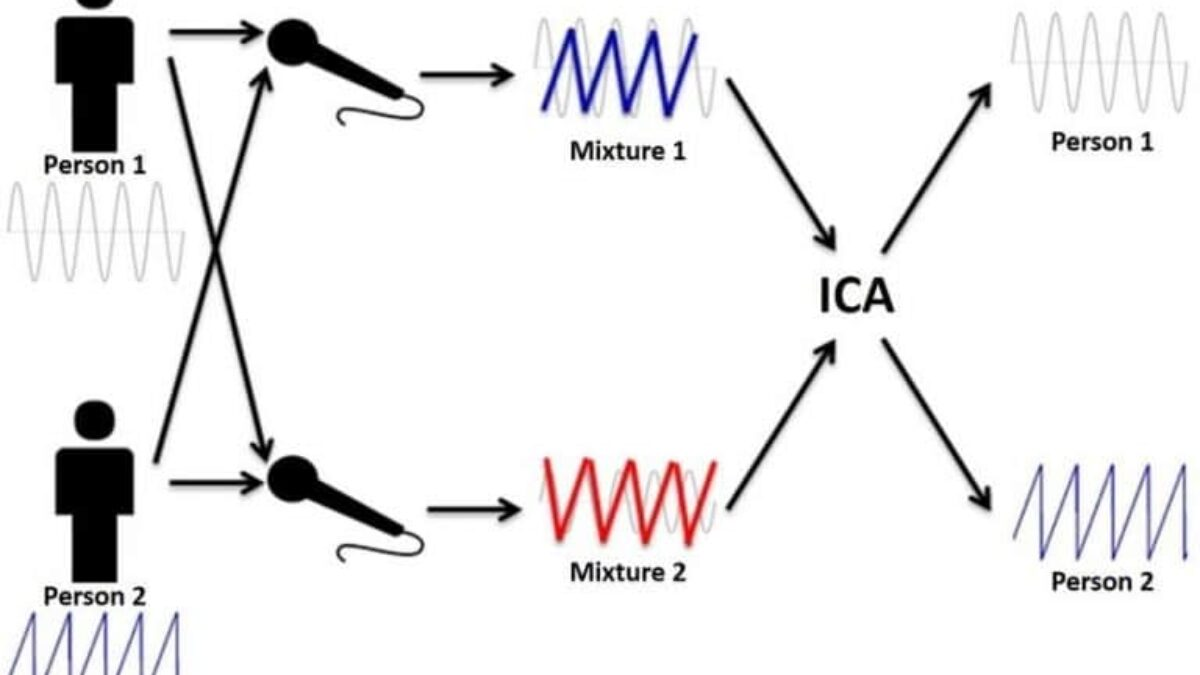
\includegraphics[width=.86\linewidth]{figures/04_ica_cocktail_party.png}
  \caption{The cocktail-party problem: both microphones record different mixtures of
  both speakers, and ICA attempts to recover the original independent signals.}
\end{figure}

In the cocktail-party picture, $\bm{y}$ holds the original voices, $\bm{U}$ is the
room (how loudly each voice reaches each microphone), and $\bm{x}$ is what the
microphones actually record.
Solving ICA means recovering $\bm{W} = \bm{U}^{-1}$ --- the un-mixing matrix ---
without ever having heard the voices separately.


\section{Identifiability and Uniqueness}
\label{sec:ica-uniqueness}

The ICA solution is generally \textbf{not fully unique}: $\bm{x} = \bm{U}\bm{P}^{-1}\bm{P}\bm{y}$
gives another valid decomposition for any invertible $\bm{P}$.
However, if $\bm{P}$ cannot mix the statistically independent components of $\bm{y}$,
then $\bm{P}$ must be a product of a permutation matrix and a diagonal scaling matrix.

\begin{thmbox}[title={Darmois' Theorem (1953) --- ICA Identifiability}]
Define $x_1 = \sum_j a_j y_j$ and $x_2 = \sum_j b_j y_j$ where $y_j$ are independent
random variables.
If $x_1$ and $x_2$ are independent, then all $y_j$ for which $a_j b_j \neq 0$ are
\emph{Gaussian}.

\medskip
Consequence: for \textbf{non-Gaussian sources}, the ICA solution is unique up to
permutation and scaling.
The Gaussian case is the only exception.
\end{thmbox}

\begin{intbox}[title={Why Gaussians kill ICA --- and why the CLT is the key}]
Take two independent standard Gaussians and plot them: you get a perfectly
circular cloud.
Now rotate that cloud by any angle you like.
It is \emph{still} a perfectly circular cloud of two independent standard
Gaussians --- you cannot tell the rotated version from the original.
The independence criterion simply has nothing to grip onto, so every rotation is
an equally valid ``solution'' and the sources are unrecoverable in principle, not
just in practice.

Non-Gaussian sources break that symmetry, and the \textbf{central limit theorem}
explains why they are recoverable.
The CLT says that summing independent variables pushes the result \emph{towards}
a Gaussian.
A mixture $\bm{a}\T\bm{y}$ is exactly such a sum --- so any mixture of the sources
is \emph{more Gaussian} than the sources themselves.
Turn that around and you get the entire ICA strategy: if mixing makes things more
Gaussian, then \textbf{un-mixing must make things less Gaussian}.
Hunt for the projection that is maximally non-Gaussian, and you will land on a
single original source.
This is why ``maximise non-Gaussianity'' and ``recover the independent sources''
are the same instruction, and it is the thread connecting kurtosis, negentropy,
and every contrast function below.
\end{intbox}

\paragraph{ICA assumptions}
\begin{itemize}
  \item Sources are \textbf{non-Gaussian} (at most one source can be Gaussian).
  \item $l \leq m$ (at least as many observations as sources).
  \item $\bm{U}$ has full rank $l$.
\end{itemize}
Source densities $p(y_i)$ are typically approximated by super-Gaussian or unimodal
distributions (generative framework).

\paragraph{Two criteria for independence}
\begin{enumerate}
  \item \textbf{Mutual information} between components.
  \item \textbf{Non-Gaussianity} of components.
\end{enumerate}


\section{Measuring Independence}

\subsection{Mutual Information}

The \textbf{mutual information} of a vector-valued random variable measures how far the
joint distribution is from a factorial (product) distribution:
\[
  I(y_1,\ldots,y_l) = \sum_{j=1}^l H(y_j) - H(\bm{y}),
\]
where $H(\bm{a}) = -\int p(\bm{a})\ln p(\bm{a})\dd\bm{a}$ is the (differential) entropy.
$I \geq 0$, with equality if and only if all components are statistically independent.

For the linear demixing $\bm{y} = \bm{W}\bm{x}$, using the change-of-variables formula
$p(\bm{y}) = p(\bm{x})/|\bm{W}|$:
\[
  I(y_1,\ldots,y_m) = \sum_{j=1}^m H(y_j) - H(\bm{x}) - \ln|\bm{W}|.
\]
Since $H(\bm{x})$ is constant in $\bm{W}$, minimizing mutual information amounts to
maximizing $\ln|\bm{W}| - \sum_j H(y_j)$, which is the ICA objective.

\subsection{Non-Gaussianity}

\paragraph{Negentropy}
The \textbf{negentropy} measures how non-Gaussian a distribution is:
\[
  J(\bm{y}) = H(\bm{y}_{\mathrm{gauss}}) - H(\bm{y}),
\]
where $\bm{y}_{\mathrm{gauss}}$ is a Gaussian with the same covariance as $\bm{y}$.
$J \geq 0$ (Gaussian has maximum entropy for fixed variance); maximizing negentropy
minimizes mutual information.
Direct estimation of negentropy is difficult in practice.

\paragraph{Kurtosis}
Non-Gaussianity can be quantified via cumulants, in particular the
\textbf{kurtosis} (fourth cumulant):
\[
  \kappa_4 = \E(x^4) - 3\bigl(\E(x^2)\bigr)^2.
\]
For a Gaussian, $\kappa_3 = \kappa_4 = 0$.
\begin{itemize}
  \item $\kappa_4 > 0$: \textbf{super-Gaussian} (heavier tails than Gaussian, e.g.\
        Laplace distribution).
  \item $\kappa_4 < 0$: \textbf{sub-Gaussian} (lighter tails, e.g.\ uniform distribution).
\end{itemize}
Key properties:
\begin{itemize}
  \item Additivity: $\kappa_4(x_1 + x_2) = \kappa_4(x_1) + \kappa_4(x_2)$ for
        independent $x_1, x_2$.
  \item Scaling: $\kappa_4(\alpha x) = \alpha^4 \kappa_4(x)$.
  \item Mixing tends to move kurtosis toward zero (towards Gaussian by the CLT).
        Therefore maximising \textbf{absolute} kurtosis can recover either super-Gaussian
        or sub-Gaussian sources; maximising signed kurtosis alone only favours the former.
\end{itemize}
Kurtosis is not robust: as a fourth-order moment, it is heavily influenced by outliers.

\paragraph{Sparseness}
For super-Gaussian sources, large positive kurtosis often corresponds to
\textbf{sparseness}: a sparse variable is usually near zero but occasionally takes large
values. This interpretation does not extend to sub-Gaussian sources such as a uniform
distribution, which have negative kurtosis but can still be separated by ICA.
Sparseness does \emph{not} imply small variance.

\paragraph{Contrast functions}
Several contrast functions are used in practice to measure non-Gaussianity:
\begin{itemize}
  \item Kurtosis: $\kappa_4(y)$.
  \item Mixed cumulants: $\frac{1}{12}\kappa_3^2(y) + \frac{1}{48}\kappa_4^2(y)$
        (normalized to zero mean, unit variance).
  \item $\left|\E_y[G(y)] - \E_\nu[G(\nu)]\right|^p$ where $\nu$ is a standard Gaussian
        and $G$ is a nonlinearity; robust choices include
        $G(x) = \log\cosh(ax)$ and $G(x) = \exp(-ax^2/2)$ with $a \geq 1$.
\end{itemize}


\section{Whitening and Rotation Algorithms}

ICA is not unique up to scaling, so the standard approach is to first remove the
scaling ambiguity by \textbf{whitening} (also called sphering), then find an
orthogonal \textbf{rotation} that maximizes non-Gaussianity.

\textbf{Whitened} data satisfies $\bm{Y}\T\bm{Y} = \bm{I}$.
Starting from $\bm{X} = \bm{Y}\bm{U}\T$ with $\bm{C} = \frac{1}{n}\bm{X}\T\bm{X}$:
\[
  \bm{I} = \bm{C}^{-1/2}\,\frac{1}{n}\bm{X}\T\bm{X}\,\bm{C}^{-1/2}
  = \frac{1}{n}\bm{C}^{-1/2}\bm{U}\,\bm{Y}\T\bm{Y}\,\bm{U}\T\bm{C}^{-1/2}.
\]
This means $\hat{\bm{U}} = \frac{1}{\sqrt{n}}\bm{C}^{-1/2}\bm{U}$ is orthogonal, and
the ICA solution decomposes as:
\[
  \bm{Y} = \frac{1}{\sqrt{n}}\,\bm{X}\,\bm{C}^{-1/2}\,\hat{\bm{U}}.
\]
The two-step procedure is:
\begin{enumerate}
  \item \textbf{Whiten:} compute $\tilde{\bm{X}} = \bm{X}\bm{C}^{-1/2}$.
  \item \textbf{Rotate:} find the orthogonal matrix $\hat{\bm{U}}$ that maximizes
        the contrast function (super-Gaussianity / sparseness).
\end{enumerate}

\begin{intbox}[title={Why split the search into whitening and rotation?}]
A general invertible mixing matrix has $m^2$ free parameters --- a big search
space.
But notice that ICA only cares about \emph{independence}, and independence
implies decorrelation.
So we can knock out the easy part first: \textbf{whitening} (a PCA-style
rescaling to unit covariance) enforces decorrelation and fixes all the stretching
and scaling for free.
Whatever freedom is left \emph{after} whitening must preserve unit covariance ---
and the only transforms that do that are \emph{rotations}.

That is the payoff: the search collapses from ``all invertible matrices'' to
``rotations only'', which is a far smaller and better-behaved space.
Whitening does the decorrelating that second-order statistics can handle, and the
rotation step then uses higher-order statistics (kurtosis, negentropy) to find
the one angle that makes the components genuinely \emph{independent}, not merely
uncorrelated.
The artificial example below makes this visible: mixing turns a square into a
parallelogram, whitening rounds it into a circle (decorrelated but still
dependent), and only the final rotation snaps it back into the axis-aligned
square.
\end{intbox}

\begin{figure}[H]
  \centering
  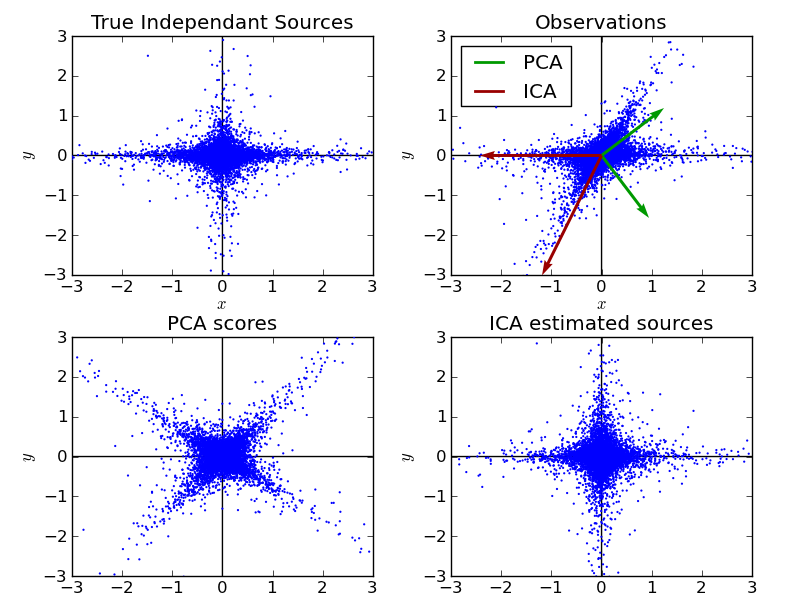
\includegraphics[width=.82\linewidth]{figures/05_ica_whitening_and_rotation.png}
  \caption{PCA decorrelates the observations but does not recover the independent axes.
  ICA uses higher-order structure to rotate the representation back towards the true
  independent sources.}
\end{figure}


\section{INFOMAX Algorithm}

\textbf{INFOMAX} (Bell \& Sejnowski, 1995) minimizes mutual information by maximizing
the entropy of a nonlinear transform of $\bm{y}$:
\[
  \bm{y} = \bm{W}\bm{x}, \qquad
  H(\bm{g}(\bm{y})) \text{ is maximized},
  \quad \bm{g}(\bm{y}) = (g(y_1),\ldots,g(y_l))\T.
\]
At maximum entropy the mutual information $I(g(y_1),\ldots,g(y_l)) = 0$, so the
components are independent.
The nonlinearity $g$ is chosen to approximate the CDF of the source distribution;
a common choice is $g(y_i) = \tanh(y_i)$ (super-Gaussian sources).

The entropy expands as
\[
  H(\bm{g}(\bm{y})) \approx H(\bm{x}) + \frac{1}{n}\sum_{i=1}^n\sum_{j=1}^l
  |\ln g'(y_{ij})| + \ln|\bm{W}|.
\]

\begin{thmbox}[title={INFOMAX Update Rules (Natural Gradient)}]
\textbf{tanh} ($g(y_j) = \tanh(y_j)$):
\[
  \Delta\bm{W} \;\propto\; \bigl(\bm{I} - 2\,\bm{g}(\bm{y})\,\bm{y}\T\bigr)\bm{W}
\]
\textbf{sigmoid} ($g(y_j) = 1/(1+e^{-y_j})$):
\[
  \Delta\bm{W} \;\propto\; \bigl(\bm{I} + (1 - 2\,\bm{g}(\bm{y}))\,\bm{y}\T\bigr)\bm{W}
\]
INFOMAX is equivalent to a generative approach using \textbf{maximum likelihood}.
\end{thmbox}

\begin{intbox}
  The natural gradient (premultiplication by $\bm{W}\T\bm{W}$) converts the
  standard gradient $(\bm{W}\T)^{-1} \pm \ldots\bm{x}\T$ into the more elegant
  update involving $\bm{y} = \bm{W}\bm{x}$.
  It also makes the algorithm \emph{equivariant}: performance does not depend on the
  scaling or conditioning of the input.
\end{intbox}


\section{EASI Algorithm}

\textbf{EASI} (Equivariant Adaptive Separation via Independence, Cardoso \& Laheld, 1996)
uses the update rule
\[
  \Delta\bm{W} \;\propto\; \bigl(\bm{I} - \bm{y}\bm{y}\T - \bm{g}(\bm{y})\bm{y}\T
  + \bm{y}\,\bm{g}\T(\bm{y})\bigr)\bm{W},
\]
where $\bm{g}$ is the same class of contrast functions as in INFOMAX (tanh or sigmoid).
EASI is designed for online learning and is also equivariant by construction.


\section{FastICA Algorithm}

\textbf{FastICA} (Hyvärinen, 1999) is probably the most widely used ICA algorithm.
It is a \emph{fixed-point} iteration (analogous to Oja's rule for PCA) that maximizes
non-Gaussianity as measured by a contrast function $g$ with derivative $g'$:

\begin{thmbox}[title={FastICA Update}]
\[
  \bm{w}^{\mathrm{new}} = \E\bigl[\bm{x}\,g(\bm{w}\T\bm{x})\bigr]
  - \E\bigl[g'(\bm{w}\T\bm{x})\bigr]\,\bm{w}.
\]
The new $\bm{w}^{\mathrm{new}}$ is then normalized to unit length.
\end{thmbox}

Key properties:
\begin{itemize}
  \item Whitening and rotation algorithm.
  \item Generalizes kurtosis maximization to arbitrary contrast functions $g$.
  \item Extended to extract multiple independent components simultaneously
        (deflation or symmetric extraction).
\end{itemize}


\section{ICA Extensions}

Beyond the basic square, invertible model several extensions exist:
\begin{itemize}
  \item \textbf{Generative approach:} assumptions on the source densities $p(y_i)$,
        sub-Gaussian sources with specific priors.
  \item \textbf{Non-linear ICA:} mixing function $\bm{x} = g(\bm{y})$ is nonlinear;
        solutions are often not unique without additional constraints.
  \item \textbf{Overcomplete ICA:} more sources than observations ($l > m$); the system
        is underdetermined but useful for sparse representations of signals.
  \item \textbf{Undercomplete ICA:} fewer sources than observations ($l < m$); reduces
        to a lower-dimensional model.
\end{itemize}


\section{ICA vs.\ PCA}

\begin{center}
\renewcommand{\arraystretch}{1.25}
\begin{tabular}{ll}
  \toprule
  \textbf{ICA} & \textbf{PCA} \\
  \midrule
  Seeks \emph{causes} of the data & Seeks \emph{geometrical abstractions} \\
  Statistically independent components & Decorrelated (orthogonal) components \\
  Fits an independent-source model & Captures directions of maximal variance \\
  Scale invariant & Not scale invariant \\
  Unique up to scaling and permutation & Unique (up to sign) \\
  Requires non-Gaussian sources (at most one Gaussian) & Uses only second-order structure \\
  Components not ranked & Components ranked by eigenvalue \\
  \bottomrule
\end{tabular}
\end{center}

\begin{intbox}
  PCA gives the best linear dimensionality reduction in terms of MSE; ICA finds the
  interpretation that is statistically most meaningful for independent source models.
  For Gaussian data both methods give the same result (any rotation of decorrelated
  Gaussians is equally independent), which is why ICA requires non-Gaussianity.
\end{intbox}


\section{Artificial ICA Examples}

Starting with 1{,}000 points from two independent \textbf{uniform distributions}
(uniform = sub-Gaussian, $\kappa_4 < 0$), the three processing stages can be visualized:

\begin{enumerate}
  \item \textbf{Original sources:} square-shaped scatter (axes-aligned).
  \item \textbf{Mixing} ($\bm{X} = \bm{Y}\bm{U}\T$): the square is rotated and sheared
        into a parallelogram/diamond shape --- the components are now dependent.
  \item \textbf{Whitening} ($\bm{X}\bm{C}^{-1/2}$): the shape becomes circular
        (unit covariance); correlation is removed but statistical dependence remains.
  \item \textbf{Rotation} (ICA): the circle is aligned back to a square, recovering
        the original independent sources.
\end{enumerate}

Both INFOMAX and FastICA recover the original square (up to permutation and sign).
For super-Gaussian sources (Laplace distribution), the shape is a four-pointed star,
and the same pipeline recovers it correctly.


\section{Real World ICA Examples}

\subsection{Iris Data Set}

On the Iris data, ICs are \textbf{ordered by their impact on the observations}
(column norms of the mixing matrix $\bm{U}$), \emph{not} by variance.
The first independent component explains approximately 90\% of the variance in the
data and likely encodes the \emph{size of the blossom} (a single dominant biological
factor).
Unlike PCA, ICA does not guarantee components are ranked by variance.

\subsection{Multiple Tissue Data Set}

Applied to the multiple tissue microarray data (102 samples, 4 tissue types), the
first three ICs provide biologically meaningful separations:
\begin{itemize}
  \item \textbf{IC1} (29\% variance): separates \emph{secretory/reproductive} tissue
        (prostate and breast) from \emph{internal organ} tissue (colon and lung) ---
        a biologically interpretable axis.
  \item \textbf{IC2} (28\%): separates prostate + lung from breast + colon.
  \item \textbf{IC3} (27\%): separates prostate + colon from breast + lung.
  \item All combinations of the first three ICs yield clean separations except for
        partial overlap between breast and lung samples.
\end{itemize}
Genes most correlated to IC1 include SERPINA7, LAMB3, \textbf{AR}, CCNG2, KLF5, CCL20,
SLC39A14, ATP1B1, GSTP1, LAD1.
The \textbf{androgen receptor} (AR) is the 3rd most related gene to IC1 --- consistent
with IC1 separating reproductive/secretory tissues, since androgen signaling drives
prostate gland differentiation and also plays a role in normal breast physiology.

\paragraph{Effect of increasing the number of components}
With 8 or 20 ICA components, the overall tissue-level separation does \emph{not}
improve relative to 4 components.
Instead, higher-order ICs focus on progressively finer-grained sub-populations
(e.g.\ specific sub-groups within colon samples), and the main tissue axes
(IC1: prostate vs.\ others; IC2: prostate+lung vs.\ breast+colon) shift in
their index but remain.
This illustrates a key difference from PCA: ICA components are not ordered
by variance, and adding more components reveals biological sub-structure rather
than explaining more total variance.


\section{Kurtosis Maximization Results in Independent Components}

The theoretical justification for kurtosis-based ICA rests on a key inequality:
the kurtosis of a linear mixture of independent variables is always less than or equal
to the \emph{maximum} kurtosis of the individual sources.
Formally, for $x = \bm{a}\T\bm{y}$ with $\|\bm{a}\| = 1$ and $y_j$ independent:
\[
  \kappa_4(x) = \sum_j a_j^4\,\kappa_4(y_j) \;\leq\; \max_j |\kappa_4(y_j)|.
\]
Equality holds when one $|a_j| = 1$ and all others are zero --- i.e.\ when the
projection aligns exactly with one source.
Therefore \textbf{maximizing $|\kappa_4|$ over all unit-norm projections recovers a
single source component}.
Iterating (deflating each recovered component) separates all sources.

\begin{notebox}[title={Limitations of kurtosis}]
Because kurtosis involves fourth moments, it is sensitive to outliers: a single
extreme data point can dominate the estimate.
More robust contrast functions such as $G(x) = \log\cosh(x)$ (used in FastICA) are
preferred in practice when outliers are expected.
\end{notebox}


% ==========================================================
\chapter{Factor Analysis}
% ==========================================================

PCA has a blind spot: it explains \emph{all} the variance in the data, and it has
no idea which part of that variance is real signal and which is measurement noise.
Point it at a noisy sensor and it will happily devote a component to the noise.

Factor analysis fixes this by being honest about noise from the start.
It splits every observed variable into two pieces: a part driven by a handful of
shared hidden \textbf{factors}, and a part that is private noise belonging to that
one variable alone.
The crucial modelling decision is that the noise covariance $\bm{\Psi}$ is
\emph{diagonal} --- noise in one measurement is independent of noise in another.
The consequence is immediate and worth pausing on: since the noise cannot create
any cross-variable correlation, \textbf{every correlation between observed
variables must be explained by the shared factors}.
That single sentence is the engine of the whole method, and it is the answer to
most conceptual exam questions about FA.

So the mental split is: \emph{factors explain what the variables have in common;
noise explains what is left over, variable by variable.}
(Get this backwards --- ``factors explain the variance, noise explains the
correlations'' --- and you have picked the classic wrong answer.)


\section{The Factor Analysis Model}

\begin{notebox}[title={Notation warning}]
This chapter writes the factor loading matrix as $\bm{\Lambda}$ and the factors as
$\bm{z}$, following the standard statistics convention.
The lecture slides and exam questions frequently use $\bm{U}$ for the loading
matrix and $\bm{y}$ for the factor vector instead --- and the FABIA chapter later
uses $U$ too.
The model is identical, only the letters change: $\bm{C}=\bm{\Lambda\Lambda}\T+\bm{\Psi}$
is the same statement as $\bm{C}=\bm{U}\bm{U}\T+\bm{\Psi}$.
\end{notebox}

\begin{defbox}[title={Factor Analysis Model}]
For centered data $\bm{x} \in \R^m$ with $l \leq m$ factors $\bm{z} \in \R^l$:
\[
  \bm{x} = \bm{\Lambda}\bm{z} + \bm{\varepsilon},
  \qquad
  \bm{z} \sim \mathcal{N}(\bm{0},\bm{I}),
  \quad
  \bm{\varepsilon} \sim \mathcal{N}(\bm{0},\bm{\Psi}),
\]
where $\bm{\Lambda} \in \R^{m \times l}$ is the \textbf{factor loading matrix} and
$\bm{\Psi} \in \R^{m \times m}$ is a \textbf{diagonal} noise covariance (so noise
components are mutually independent).
The model gives $\bm{x} \mid \bm{z} \sim \mathcal{N}(\bm{\Lambda}\bm{z},\bm{\Psi})$.
\end{defbox}

\paragraph{Covariance decomposition}
\figureplaceholder
  {Factor analysis separates shared factors from variable-specific noise.}
  {A graphical model with a few latent factors pointing to several observed variables, plus one private noise node per observation. Next to it, show covariance as low-rank shared covariance plus diagonal noise.}
  {factor analysis graphical model latent factors unique variance diagram}

Marginalising over $\bm{z}$ gives $\bm{x} \sim \mathcal{N}(\bm{0},\, \bm{\Lambda}\bm{\Lambda}\T+\bm{\Psi})$.
The model-implied covariance is compared with the sample covariance
$\bm{C} = \frac{1}{n}\bm{X}\T\bm{X}$:
\[
  \bm{C} \;\approx\; \bm{\Lambda}\bm{\Lambda}\T + \bm{\Psi}.
\]
FA is therefore a \textbf{decomposition of the covariance matrix}: $\bm{\Lambda}$
captures the shared (dependent) variance; $\bm{\Psi}$ captures the unique
(independent) variance per variable.
Because $\bm{\Psi}$ is diagonal, all correlations between observations can
\emph{only} be explained by the factors.

In matrix form, $\bm{X} = \bm{Z}\bm{\Lambda}\T + \bm{E}$ with model assumptions
$\frac{1}{n}\bm{Z}\T\bm{Z} = \bm{I}$, $\bm{Z}\T\bm{E} = \bm{0}$, and
$\frac{1}{n}\bm{E}\T\bm{E} = \bm{\Psi}$.

\paragraph{Factor scores (estimation)}
Treating factor recovery as regression $\bm{Y} = \bm{X}\bm{A}$ and using the
model approximations $\frac{1}{n}\bm{X}\T\bm{X} \approx \bm{\Lambda}\bm{\Lambda}\T+\bm{\Psi}$
and $\frac{1}{n}\bm{X}\T\bm{Y} \approx \bm{\Lambda}$:
\[
  \hat{\bm{A}} = (\bm{\Lambda}\bm{\Lambda}\T + \bm{\Psi})^{-1}\bm{\Lambda},
  \qquad
  \bm{Y} = \bm{X}(\bm{\Lambda}\bm{\Lambda}\T+\bm{\Psi})^{-1}\bm{\Lambda}.
\]
Applying the matrix inversion lemma to avoid inverting the $m\times m$ matrix:
\[
  \bm{Y} = \bm{X}\,\bm{\Psi}^{-1}\bm{\Lambda}\,(\bm{I} + \bm{\Lambda}\T\bm{\Psi}^{-1}\bm{\Lambda})^{-1}.
\]

\paragraph{Communality}
The \textbf{communality} of observation variable $x_j$ is the proportion of its
variance explained by the factors:
\[
  c_j = \frac{\mathrm{Var}(x_j) - \mathrm{Var}(\varepsilon_j)}{\mathrm{Var}(x_j)}
      = \frac{\sum_{k=1}^l \lambda_{jk}^2}{\Psi_{jj} + \sum_{k=1}^l \lambda_{jk}^2}.
\]
Factor $z_t$ individually contributes $\lambda_{jt}^2 / (\Psi_{jj} + \sum_k \lambda_{jk}^2)$
to $x_j$.
Like PCA, projecting onto $l$ factors maximizes the variance that can be explained by $l$
factors --- but FA counts only signal variance, not noise.

\paragraph{Rotation non-identifiability}
The FA loading matrix is \textbf{not identifiable}: every orthogonal rotation gives
the same marginal covariance and likelihood,
$\bm{\Lambda}\bm{z} = \bm{\Lambda}\bm{V}\bm{V}\T\bm{z} = \bm{\Lambda}'\bm{z}'$
for any orthogonal $\bm{V}$.
Rotations are therefore chosen to improve interpretability:
\begin{itemize}
  \item \textbf{Varimax}: simplifies columns of the loading matrix, encouraging each
        factor to have a small set of large loadings and many near-zero loadings.
  \item \textbf{Quartimax}: simplifies rows, encouraging each variable to load strongly
        on only a small number of factors; it can produce one broad general factor.
  \item \textbf{Equimax}: a compromise between Varimax and Quartimax.
\end{itemize}


\section{Maximum Likelihood Factor Analysis}

Since $\bm{x} \sim \mathcal{N}(\bm{0},\bm{\Lambda}\bm{\Lambda}\T+\bm{\Psi})$,
the log-likelihood over $n$ samples is
\[
  \ln\mathcal{L}(\bm{\Lambda},\bm{\Psi}) =
  \sum_{i=1}^n \left[
    -\tfrac{m}{2}\ln(2\pi)
    -\tfrac{1}{2}\ln|\bm{\Lambda}\bm{\Lambda}\T+\bm{\Psi}|
    -\tfrac{1}{2}(\bm{x}^i)\T(\bm{\Lambda}\bm{\Lambda}\T+\bm{\Psi})^{-1}\bm{x}^i
  \right].
\]
Maximising this has \textbf{no closed form}, so the \textbf{EM algorithm} is used with
the latent factors $\bm{z}^i$ as the hidden variables.

\begin{thmbox}[title={FA EM Algorithm}]
\textbf{E-step:} compute the posterior of the factors for each sample (using the
Gaussian conditional formula):
\[
  \bm{z}^i \mid \bm{x}^i \;\sim\; \mathcal{N}(\bm{\mu}_{\bm{z}|{\bm{x}^i}},\;\bm{\Sigma}_{\bm{z}|\bm{x}}),
\]
\[
  \bm{\mu}_{\bm{z}^i|\bm{x}^i} = (\bm{x}^i)\T (\bm{\Lambda}\bm{\Lambda}\T+\bm{\Psi})^{-1}\bm{\Lambda},
  \qquad
  \bm{\Sigma}_{\bm{z}|\bm{x}} = \bm{I} - \bm{\Lambda}\T(\bm{\Lambda}\bm{\Lambda}\T+\bm{\Psi})^{-1}\bm{\Lambda}.
\]
Note: the posterior covariance $\bm{\Sigma}_{\bm{z}|\bm{x}}$ is the same for all
data points (it does not depend on $\bm{x}^i$).

\textbf{M-step:} update the parameters by setting gradients to zero:
\[
  \bm{\Lambda}^{\mathrm{new}} =
    \Bigl(\tfrac{1}{n}\sum_{i=1}^n \bm{x}^i\,\E_{\bm{z}^i|\bm{x}^i}[\bm{z}^i]\T\Bigr)
    \Bigl(\tfrac{1}{n}\sum_{i=1}^n \E_{\bm{z}^i|\bm{x}^i}[\bm{z}^i(\bm{z}^i)\T]\Bigr)^{-1},
\]
\[
  \bm{\Psi}^{\mathrm{new}} = \tfrac{1}{n}\,\mathrm{diag}\!\Bigl(
    \sum_{i=1}^n \bm{x}^i(\bm{x}^i)\T
    - \sum_{i=1}^n \E_{\bm{z}^i|\bm{x}^i}[\bm{z}^i]\,\bm{x}^i (\bm{\Lambda}^{\mathrm{new}})\T
  \Bigr),
\]
where $\E[\bm{z}^i(\bm{z}^i)\T] = \bm{\mu}_{\bm{z}^i|\bm{x}^i}\bm{\mu}_{\bm{z}^i|\bm{x}^i}\T + \bm{\Sigma}_{\bm{z}|\bm{x}}$.
\end{thmbox}

\paragraph{Matrix inversion speedup}
When $m \gg l$, directly inverting the $m\times m$ matrix
$(\bm{\Lambda}\bm{\Lambda}\T + \bm{\Psi})$ is expensive.
The matrix inversion lemma gives an $l\times l$ inversion instead:
\[
  (\bm{\Lambda}\bm{\Lambda}\T + \bm{\Psi})^{-1}
  = \bm{\Psi}^{-1} - \bm{\Psi}^{-1}\bm{\Lambda}
    (\bm{I} + \bm{\Lambda}\T\bm{\Psi}^{-1}\bm{\Lambda})^{-1}
    \bm{\Lambda}\T\bm{\Psi}^{-1}.
\]
Since $\bm{\Psi}$ is diagonal, $\bm{\Psi}^{-1}$ is trivially cheap.
Furthermore the sample covariance $\bm{C}$ only needs to be computed once per
EM run.


\section{Factor Analysis vs.\ PCA and ICA}

\begin{center}
\renewcommand{\arraystretch}{1.25}
\begin{tabular}{lll}
  \toprule
  & \textbf{FA} & \textbf{PCA / ICA} \\
  \midrule
  Noise model & Explicit Gaussian noise $\bm{\Psi}$ & None (PCA: no noise; ICA: no noise) \\
  Factors/sources & Gaussian priors $\mathcal{N}(\bm{0},\bm{I})$ & PCA: none; ICA: non-Gaussian \\
  Objective & Max.\ signal variance (covariance fit) & PCA: all variance; ICA: independence \\
  Uniqueness & Rotation-indeterminate & PCA: up to sign; ICA: up to scale/permutation \\
  Estimation & EM (no closed form) & PCA: eigen; ICA: gradient/fixed-point \\
  \bottomrule
\end{tabular}
\end{center}

\begin{intbox}
  FA is the right choice when you believe observations contain genuine measurement
  noise that should be separated from the latent signal.
  PCA absorbs noise into the components (it explains \emph{all} variance, noise
  included), while FA explicitly models it via $\bm{\Psi}$.
  ICA additionally demands statistical independence of the sources and therefore
  requires non-Gaussian source distributions.
\end{intbox}


\section{Artificial Factor Analysis Examples}

To see when FA fails, consider 50-dimensional data generated from two independent
\textbf{super-Gaussian} (Laplacian) latent sources.
In 2-D projection the two sources form a characteristic ``star'' or diamond
shape (uniform mass on four arms), which reflects their non-Gaussian
character.

\textbf{ICA} correctly recovers this star shape: because the true sources are
statistically independent and non-Gaussian, the ICA objective (contrast function
or kurtosis) can identify them.

\textbf{FA} with two factors does \emph{not} recover the star.
FA's generative model assumes the latent factors $\bm{z}$ are Gaussian. It can still
recover a useful low-dimensional subspace and covariance structure, but covariance alone
cannot choose the particular rotation corresponding to independent non-Gaussian sources.
ICA uses higher-order information to identify that rotation.

\begin{intbox}[title={Why FA fails for non-Gaussian sources}]
FA is the maximum-likelihood model when factors are Gaussian.
Forcing super-Gaussian data into a Gaussian-factor likelihood throws away the feature
that identifies the axes: non-Gaussian shape. EM may fit the covariance well while
returning a rotated version of the sources. ICA is preferable when the goal is
specifically to recover independent, non-Gaussian causes.
\end{intbox}


\section{Real World Factor Analysis Examples}

\subsection{Iris Data Set}

In the lecture's Iris analysis, a \textbf{one-factor} model captures much of the dominant
size-related variation. Its factor scores separate \textit{setosa} strongly and order the
other two species, but one should not read this as a general guarantee of clean class
separation: FA is unsupervised and never sees the species labels.

\subsection{Multiple Tissue Data Set}

With \textbf{four factors} and no rotation the four components have distinct
biological interpretations:
\begin{itemize}
  \item \textbf{FA1} — cleanly separates prostate samples.
  \item \textbf{FA2} — partially separates breast from lung, but the overlap is
        substantial.
  \item \textbf{FA3} — separates colon samples.
  \item \textbf{FA4} — separates a subset of lung samples.
\end{itemize}

Applying \textbf{Varimax} rotation to the four factors changes the factor axes
but does not change the overall fit.
The pairwise scatter plots (all six pairs among FA1–FA4) show that
\emph{separation is slightly worse} than without rotation: the rotation mixes
biological signal across components rather than concentrating it.

\textbf{Quartimax} rotation gives a result similar to Varimax — the separation
quality is again slightly worse than the unrotated solution.

\begin{intbox}[title={Rotation does not help here}]
Rotation methods such as Varimax and Quartimax search for a sparse, interpretable
factor loading matrix.
On this data the unrotated MLE already concentrates each factor on one tissue
type, so rotation does not improve tissue separation and can even dilute it.
Rotation is most valuable when the unrotated factors are hard to interpret
biologically.
\end{intbox}


% ==========================================================
\chapter{Scaling and Projection Methods}
% ==========================================================

Every method in this chapter squeezes high-dimensional data down into a few
dimensions --- usually two, so you can actually look at it.
The reason to care is that we cannot see in 5{,}000 dimensions, and a great deal
of data analysis begins with wanting to \emph{look} at the thing.

What separates the methods is a single question: \textbf{what are you trying to
preserve on the way down?}
Everything in this chapter is an answer to that question, and once you see it
that way the zoo becomes a short list:

\begin{itemize}
  \item \textbf{Projection pursuit} --- preserve \emph{interestingness}
        (non-Gaussianity).
  \item \textbf{MDS} --- preserve \emph{pairwise distances}.
  \item \textbf{Isomap} --- preserve pairwise distances, but measured
        \emph{along the manifold} (geodesics) rather than through empty space.
  \item \textbf{LLE} --- preserve each point's \emph{local linear relationship}
        to its neighbours.
  \item \textbf{$t$-SNE} --- preserve \emph{neighbourhood probabilities}, with a
        deliberate trick to stop everything crowding together.
  \item \textbf{SOM / GTM} --- preserve \emph{topology}, by pinning the projection
        to a grid of latent points.
  \item \textbf{NMF} --- not a projection to visualise, but a decomposition into
        \emph{additive parts}.
\end{itemize}

Two warnings that recur throughout, and that exams like to probe.
\figureplaceholder
  {What the main projection methods try to preserve.}
  {A single Swiss-roll data set shown with four overlays: straight Euclidean distances for MDS, neighbour reconstruction weights for LLE, graph geodesics for Isomap, and local similarity probabilities for t-SNE.}
  {PCA MDS LLE Isomap t-SNE comparison Swiss roll}

First, the projection always goes to a \emph{lower}-dimensional space --- any
statement claiming these methods project \emph{up} in order to spread points apart
is a distractor.
Second, a manifold method is only as good as its assumption: the last few sections
show LLE, Isomap, and $t$-SNE all doing beautifully on Swiss rolls and digit
images, then all failing on the gene-expression data --- because that data simply
does not lie on a smooth low-dimensional manifold.

\section{Projection Pursuit}

\textbf{Projection pursuit} asks: among all linear projections
$t = \bm{w}\T\bm{x}$ (normalised to zero mean, unit variance), which
direction $\bm{w}$ is most \emph{interesting}?
The classical answer is: the \textbf{least Gaussian} direction.

The rationale comes from information theory: among all distributions with
a fixed mean and covariance, the Gaussian maximises entropy.
Consequently, a projection that looks close to Gaussian is ``boring'' —
it carries no structure beyond the second-order statistics already captured
by PCA.
A projection with low entropy (far from Gaussian) reveals genuine
non-linear or non-Gaussian structure.

\begin{defbox}[title={Projection Pursuit Objective}]
Find $\bm{w}$ that minimises the differential entropy $H(t)$ of the projected
variable $t = \bm{w}\T\bm{x}$, subject to $\mathrm{Var}(t)=1$.
\end{defbox}

This optimisation is difficult in practice because it requires estimating a
density.
Two qualitatively different types of structure can be found:
\begin{itemize}
  \item \textbf{Unimodal super-Gaussians} — heavy-tailed, peaked distributions
        (single cluster with outliers).
  \item \textbf{Multimodal distributions} — several separated clusters.
\end{itemize}
In practice, projection pursuit uses the same contrast functions as ICA —
kurtosis, negentropy approximations — as tractable surrogates for $H(t)$.
Projection pursuit can therefore be seen as a precursor to ICA; ICA adds the
constraint that multiple projected directions must be mutually independent.


\section{Multidimensional Scaling}

\subsection{The Method}

\textbf{Multidimensional scaling} (MDS) projects data to a low-dimensional
target space $\bm{y}_i = f(\bm{x}_i;\bm{w})$ while keeping the
\emph{pairwise distances} between points as intact as possible.

Define:
\[
  \delta_{ij} = \|\bm{x}_i - \bm{x}_j\|
  \quad\text{(original distances)},\qquad
  d_{ij} = \|\bm{y}_i - \bm{y}_j\|
  \quad\text{(projected distances)}.
\]
The goal is $d \approx \delta$.
Different \textbf{stress measures} formalise the mismatch:

\begin{align*}
  R_1(d,\delta) &= \frac{\displaystyle\sum_{i<j}(d_{ij}-\delta_{ij})^2}
                        {\displaystyle\sum_{i<j}\delta_{ij}^2}
  && \text{(Kruskal's measure — penalises large absolute errors)} \\[6pt]
  R_2(d,\delta) &= \sum_{i<j}\!\left(\frac{d_{ij}-\delta_{ij}}{\delta_{ij}}\right)^{\!2}
  && \text{(fractional/relative errors)} \\[6pt]
  R_3(d,\delta) &= \frac{1}{\displaystyle\sum_{i<j}\delta_{ij}}
                   \sum_{i<j}\frac{(d_{ij}-\delta_{ij})^2}{\delta_{ij}}
  && \text{(Sammon mapping — compromise)}
\end{align*}

These stress objectives can be minimised iteratively, but not every MDS variant needs
gradient descent: classical metric MDS has the eigendecomposition solution described
below, while non-metric MDS additionally fits monotone disparities to the observed
dissimilarities.
The gradient of $R_1$ with respect to the projected position $\bm{y}_k$ is:
\[
  \frac{\partial}{\partial\bm{y}_k}R_1
  = \frac{2}{\sum_{i<j}\delta_{ij}^2}
    \sum_{j\neq k}(d_{kj}-\delta_{kj})\,\frac{\bm{y}_k-\bm{y}_j}{d_{kj}},
\]
and analogous expressions hold for $R_2$ and $R_3$ (replacing the weight by
$1/\delta_{kj}^2$ or $1/\delta_{kj}$, respectively).
Viewing $R$ as a potential energy, the gradients are \textbf{forces} that push
or pull each point toward its correct distance from every other point.

A special case is \textbf{metric MDS} (also called \emph{principal coordinates
analysis}): when distances are Euclidean and one seeks a linear embedding,
the optimal solution can be computed analytically via eigendecomposition of the
centred distance matrix — no gradient descent is needed.

\subsection{Examples}

MDS is applied to the \textbf{Multiple Tissue} gene-expression data set (four
tissue types: colon, lung, breast, prostate).
The 101 or 13 genes with the largest variance across samples are selected as
features.

\begin{itemize}
  \item \textbf{Metric MDS} (101 features): colon samples (orange) cluster in
        the upper-left; prostate (green) separates to the right; lung (blue) and
        breast (red) form an overlapping cluster in the lower region.
        Using only 13 features gives a similar layout.

  \item \textbf{Kruskal's non-metric MDS} (101 and 13 features): the
        separation pattern is qualitatively the same as metric MDS.

  \item \textbf{Sammon's non-linear mapping} (101 features): the tissue groups
        are less well separated than with metric or Kruskal's measure.
        With only 13 features the clusters are \emph{more spread out}, but the
        qualitative separation is still inferior to the other variants.
\end{itemize}

Overall, metric MDS and Kruskal's non-metric MDS perform similarly on this
data set, and both outperform Sammon's mapping.

\section{Non-negative Matrix Factorization}

\subsection{The Method}

\textbf{Non-negative matrix factorization} (NMF) approximates a non-negative
data matrix $\bm{X}\in\mathbb{R}^{n\times m}$ ($X_{ij}\geq 0$) as
\[
  \bm{X} \;\approx\; \bm{Y}\bm{U}\T
  \;=\; \sum_{k=1}^{l} \bm{y}_k\,\bm{u}_k\T,
\]
where $\bm{Y}\in\mathbb{R}^{n\times l}$ and $\bm{U}\in\mathbb{R}^{m\times l}$
are also required to be non-negative ($Y_{ik}\geq 0$, $U_{jk}\geq 0$).

The non-negativity constraint encourages an additive, often \textbf{parts-based
representation}:
every observation is reconstructed by \emph{adding} non-negative parts, never
by subtraction. Localised semantic parts are a common outcome, not a mathematical
guarantee.
This contrasts with PCA, whose eigenvectors can have both signs, producing
holistic (whole-image) components.

\begin{figure}[H]
  \centering
  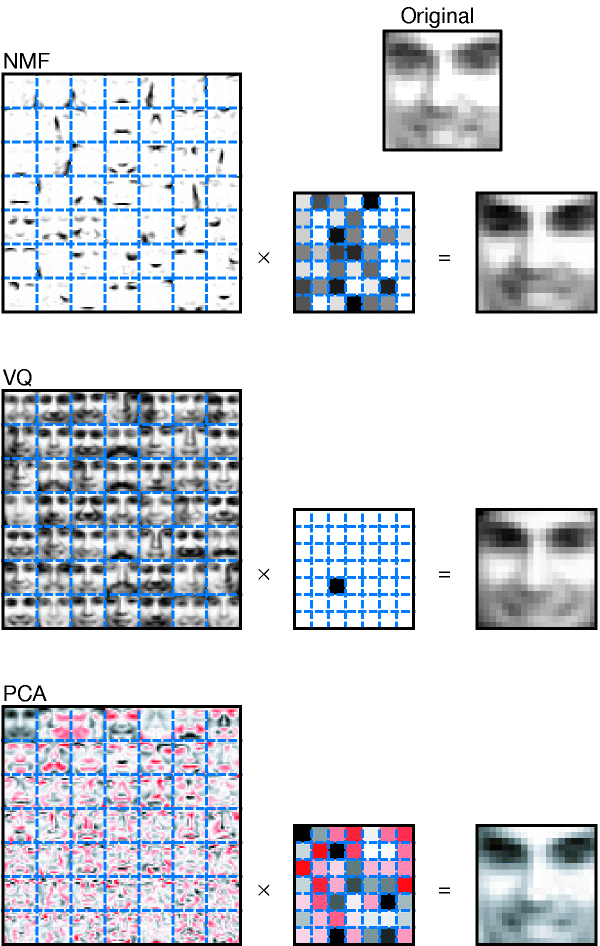
\includegraphics[width=.82\linewidth,trim=0 590bp 0 0,clip]{figures/07_nmf_parts_based_faces.png}
  \caption{NMF reconstructs a face by combining non-negative, spatially localised
  basis parts with non-negative activation weights.}
\end{figure}

\paragraph{Multiplicative update rules}

Two objectives are in common use.

\textbf{Objective 1 — KL divergence.}
For non-negative matrices normalised to sum to one:
\[
  D(\bm{A}\|\bm{B})
  = \sum_{ij}\Bigl(A_{ij}\log\frac{A_{ij}}{B_{ij}} - A_{ij} + B_{ij}\Bigr).
\]
Minimising $D(\bm{X}\|\bm{Y}\bm{U}\T)$ leads to multiplicative updates:
\[
  Y_{ik} \;\leftarrow\; Y_{ik}\,
    \frac{\displaystyle\sum_{j=1}^{m} U_{jk}\,X_{ij}/(\bm{Y}\bm{U}\T)_{ij}}
         {\displaystyle\sum_{j=1}^{m} U_{jk}},
  \qquad
  U_{jk} \;\leftarrow\; U_{jk}\,
    \frac{\displaystyle\sum_{i=1}^{n} Y_{ik}\,X_{ij}/(\bm{Y}\bm{U}\T)_{ij}}
         {\displaystyle\sum_{i=1}^{n} Y_{ik}}.
\]

\textbf{Objective 2 — Frobenius norm.}
$\|\bm{X}-\bm{Y}\bm{U}\T\|_F^2 = \sum_{ij}(X_{ij}-(\bm{Y}\bm{U}\T)_{ij})^2$.
Multiplicative updates are obtained by multiplying the
fixed-point condition $\bm{X}=\bm{Y}\bm{U}\T$ from the right by $\bm{U}$
(for $\bm{Y}$) or from the left by $\bm{Y}\T$ (for $\bm{U}$):
\[
  Y_{ik} \;\leftarrow\; Y_{ik}\,
    \frac{(\bm{X}\bm{U})_{ik}}{(\bm{Y}\bm{U}\T\bm{U})_{ik}},
  \qquad
  U_{jk} \;\leftarrow\; U_{jk}\,
    \frac{(\bm{Y}\T\bm{X})_{kj}}{(\bm{Y}\T\bm{Y}\bm{U}\T)_{kj}}.
\]
At a fixed point the left and right sides are equal.

\begin{intbox}[title={Why multiplicative updates preserve non-negativity}]
Both update rules multiply each entry by a ratio of non-negative quantities.
Starting from a non-negative initialisation, all entries remain non-negative
throughout training.
\end{intbox}

NMF can be extended to \textbf{sparse NMF}, adding sparsity penalties on
$\bm{Y}$ (few parts active per sample) and/or $\bm{U}$ (each part described
by few features).
In gene-expression analysis this corresponds to: part = pathway, few genes
participate in each pathway, and only few pathways are active per sample.

\subsection{Examples}

\paragraph{Parts-based face representation.}
Applied to a face database, NMF learns \emph{local face parts} (eye regions,
nose patches, mouth shapes).
Vector quantisation (VQ) and PCA both learn holistic representations — entire
faces or signed global components.
The parts-based decomposition from NMF is more interpretable for many
real-world objects.

\paragraph{Bicluster recovery (FABIA toy data).}
A synthetic data matrix (1{,}000 genes, 100 samples, 13 biclusters) generated
by the FABIA biclustering package provides a ground-truth test bed.
The blocks of elevated expression are localised in specific gene/sample
subsets; the background is near zero.

\begin{itemize}
  \item \textbf{NMF (KL divergence, NMFDIV)}: reconstructs the block structure
        well with small residual noise.
        The absolute factors and loadings matrices each show sparse, localised
        activity corresponding to individual biclusters.
  \item \textbf{NMF (Euclidean distance, NMFEU)}: similarly good reconstruction;
        the residual error is small and structureless.
  \item \textbf{Sparse NMF (NMFSC)}: enforcing sparseness misses some blocks
        entirely when the sparseness parameter is too large.
        The loadings matrix becomes nearly uniform across all genes (columns look
        identical) — the method cannot distinguish which genes belong to which
        bicluster.
        The takeaway is that \emph{the sparseness parameter is difficult to tune};
        too little gives the same result as plain NMF, too much destroys the
        bicluster structure.
  \item \textbf{FABIA biclustering}: the FABIA model (Chapter~8) recovers the
        bicluster structure more faithfully than any NMF variant, with sharper
        factor and loading matrices.
\end{itemize}

\section{Locally Linear Embedding}

\subsection{The Method}

\textbf{Locally linear embedding} (LLE) computes a low-dimensional,
neighbourhood-preserving embedding via a nonlinear mapping.
The key insight is that on a smooth manifold, each point can be approximated
by a linear combination of its nearest neighbours; LLE finds the embedding
that \emph{preserves} those local linear relationships.

\paragraph{Step 1 — compute reconstruction weights.}
For each point $\bm{x}_i$, find $k$ nearest neighbours and solve for weights
$W_{ij}$ that best reconstruct $\bm{x}_i$ from its neighbours:
\[
  \varepsilon(\bm{W}) = \sum_i \left\|\bm{x}_i
    - \sum_{j=1}^{k} W_{ij}\,\bm{x}_j\right\|^2,
  \quad\text{subject to}\quad \sum_{j=1}^{k} W_{ij} = 1.
\]
The sum-to-one constraint makes the weights invariant to translations; uniform
rotations and rescalings multiply the local least-squares objective without changing
its minimiser. For point $i$, form the centred neighbour matrix from vectors
$\bm{x}_i-\bm{x}_j$ and its local Gram matrix
$C^{(i)}_{jk}=(\bm{x}_i-\bm{x}_j)\T(\bm{x}_i-\bm{x}_k)$. The optimal neighbour weights
have the compact form
\[
  \bm{w}_i = \frac{(\bm{C}^{(i)})^{-1}\mathbf{1}}
                   {\mathbf{1}\T(\bm{C}^{(i)})^{-1}\mathbf{1}},
\]
with all non-neighbour weights set to zero. In practice one solves this linear system
rather than forming the inverse explicitly.

\paragraph{Step 2 — compute the embedding.}
Hold the weights $W_{ij}$ fixed and find low-dimensional coordinates
$\bm{y}_i$ that minimise the same reconstruction error:
\[
  \Phi(\bm{Y}) = \sum_{ij} M_{ij}\,\bm{y}_i\T\bm{y}_j,
  \quad\text{where}\quad
  M_{ij} = \delta_{ij} - W_{ij} - W_{ji} + \sum_k W_{ki}W_{kj},
\]
which can be written compactly as $\bm{M}=(\bm{I}-\bm{W})\T(\bm{I}-\bm{W})$.
Because the row sums of $\bm{W}$ are one, $(\bm{I}-\bm{W})\mathbf{1}=\mathbf{0}$,
so $\bm{M}$ always has a zero eigenvalue with eigenvector $\mathbf{1}$.
The optimal $d$-dimensional embedding consists of the \emph{bottom} $d$
eigenvectors of $\bm{M}$ (those with the $d$ smallest non-zero eigenvalues);
the trivial zero eigenvector is discarded.

\begin{intbox}[title={LLE implementation notes}]
\begin{itemize}
  \item Neighbours can be found by $k$-NN (Euclidean), $\varepsilon$-ball, or
        KD trees for efficiency.
  \item If $k>m$ the local covariance $\bm{C}$ is rank-deficient; regularise
        with $\bm{C}\leftarrow\bm{C}+\varepsilon\bm{I}$ where
        $\varepsilon\approx 10^{-3}\operatorname{tr}(\bm{C})$.
  \item The matrix $\bm{M}$ is sparse (only $k$ off-diagonal entries per row),
        so its eigenvectors can be computed efficiently.
\end{itemize}
\end{intbox}

\subsection{Examples}

LLE succeeds on data that genuinely lives on a smooth low-dimensional manifold.

\textbf{Swiss Roll.} LLE ``unrolls'' the 3-D spiral manifold into a flat 2-D
rectangle, recovering the original 2-D parameterisation of the roll.

\textbf{Face images.} Applied to a large collection of face photographs, LLE
produces a 2-D embedding in which one axis encodes head pose and the other
encodes expression or illumination — a smooth manifold structure in pixel space.

\textbf{``S'' curve.} On a 3-D S-shaped surface LLE fails to produce a clean
unrolling; the embedded scatter plot is disordered.

\textbf{Multiple Tissue (gene expression).} With $k\in\{5,7,9,12\}$, LLE gives
poor tissue separation in all cases.
The four tissue types are not concentrated on a low-dimensional manifold in
gene-expression space — they are spread throughout the high-dimensional space —
so LLE's assumption is violated.

\section{Isomap}

\subsection{The Method}

\textbf{Isomap} computes a quasi-isometric low-dimensional embedding.
Like LLE it is a non-linear projection, but instead of preserving local
linear relationships it preserves \textbf{geodesic distances} — shortest
paths along the data manifold.

\paragraph{Why geodesic rather than Euclidean?}
For data lying on a curved manifold, the straight-line Euclidean distance
between two far-apart points cuts through empty space and underestimates the
true manifold distance.
The geodesic distance follows the surface and is a better measure of
``closeness'' on the manifold.

\paragraph{Algorithm.}
\begin{enumerate}
  \item \textbf{Build the neighbourhood graph $G$.} Connect $\bm{x}_i$ and
        $\bm{x}_j$ if $d(\bm{x}_i,\bm{x}_j)<\varepsilon$ ($\varepsilon$-Isomap)
        or if $i$ is among the $k$ nearest neighbours of $j$ ($k$-Isomap).
        Set each edge length to $d(\bm{x}_i,\bm{x}_j)$.
  \item \textbf{Compute all-pairs shortest paths} using Floyd's algorithm:
        initialise $d_G(\bm{x}_i,\bm{x}_j)=d(\bm{x}_i,\bm{x}_j)$ for linked
        pairs and $\infty$ otherwise, then iterate
        \[d_G(\bm{x}_i,\bm{x}_j)\leftarrow
          \min\bigl(d_G(\bm{x}_i,\bm{x}_j),\;
                    d_G(\bm{x}_i,\bm{x}_k)+d_G(\bm{x}_k,\bm{x}_j)\bigr).\]
        Store the result as the geodesic distance matrix $\bm{D}_X$.
  \item \textbf{Compute the embedding.} Convert distances to inner products via
        the doubly-centred transform
        \[\tau(\bm{D}) = -\tfrac{1}{2}\,\bm{H}\,\bm{D}^2\,\bm{H},\qquad
          \bm{H}=\bm{I}_n-\tfrac{1}{n}\mathbf{1}\mathbf{1}\T,\]
        where $\bm{D}^2$ is the element-wise square of $\bm{D}$.
        The embedding coordinates are given by
        $y_{ij}=\sqrt{\lambda_p}\,v_{ji}$,
        where $\lambda_p$ and $v_p$ are the $p$-th largest eigenvalue and
        eigenvector of $\tau(\bm{D}_X)$.
\end{enumerate}

The objective that is minimised is
$E=\|\tau(\bm{D}_X)-\tau(\bm{D}_Y)\|_{L^2}$, where
$\bm{D}_Y$ collects Euclidean distances in the projected space.
Setting the embedding to the top-$l$ eigenvectors of $\tau(\bm{D}_X)$ is the
exact analytic solution.

\subsection{Examples}

\textbf{Hand images.} $n=2{,}000$ images of a hand opening and closing at
varying wrist orientations ($k=6$).
Isomap recovers the underlying two-dimensional manifold: one axis encodes
\emph{wrist rotation}, the other \emph{finger extension} — a semantically
meaningful 2-D embedding of a high-dimensional image space.

\textbf{Tree-count data (Barro Colorado Island).} 50 one-hectare plots, 225
tree species.
Classical metric MDS (cmdscale), $k$-Isomap ($k=3$, $k=5$), and
$\varepsilon$-Isomap ($\varepsilon=0.45$) give qualitatively different layouts
of the 50 plots in 2-D.
The neighbourhood parameter strongly influences the result.

\textbf{Multiple Tissue.}
Results are not as good as with linear methods (metric MDS, FA) for any
setting of $\varepsilon$.
As with LLE, the gene-expression data do not lie on a smooth manifold, so
geodesic-distance-based methods gain nothing over Euclidean methods and may
even perform worse.

\section{The Generative Topographic Mapping}%
\label{sec:gtm}

\subsection{The Method}

The \textbf{Generative Topographic Mapping} (GTM) is a probabilistic,
non-linear latent variable model designed as a principled alternative to
Self-Organising Maps (SOMs).
Like FA, GTM maps from a low-dimensional latent space to the observation space;
unlike FA the mapping $\bm{x}(\bm{y};\bm{w})$ is nonlinear.

Latent variables $\bm{y}\in\mathbb{R}^l$ are mapped to a manifold
$\mathcal{S}$ embedded in $\mathbb{R}^m$ ($m>l$).
Because a deterministic map from an $l$-dimensional space to an
$m$-dimensional space concentrates all probability mass on a zero-volume
surface (probability densities vanish), GTM places a \textbf{Gaussian ball}
around each mapped point:
\[
  p(\bm{t}\mid\bm{y},\bm{w},\beta)
  = \left(\frac{\beta}{2\pi}\right)^{m/2}
    \exp\!\left(-\frac{\beta}{2}\|\bm{x}(\bm{y},\bm{w})-\bm{t}\|^2\right).
\]

The marginal density over observations is obtained by integrating over the
latent space:
\[
  p(\bm{t}\mid\bm{w},\beta) = \int p(\bm{t}\mid\bm{y},\bm{w},\beta)\,p(\bm{y})\,\mathrm{d}\bm{y}.
\]

In practice the latent prior $p(\bm{y})$ is approximated by a uniform discrete
distribution over $L$ grid points $\{\bm{y}_j\}$:
\[
  p(\bm{y}) = \frac{1}{L}\sum_{j=1}^L \delta(\bm{y}-\bm{y}_j),
  \qquad
  p(\bm{t}\mid\bm{w},\beta) = \frac{1}{L}\sum_{j=1}^L
    p(\bm{t}\mid\bm{y}_j,\bm{w},\beta).
\]
This is a \textbf{constrained Gaussian mixture model} in $\mathbb{R}^m$: the
$L$ mixture centres are not free but must all lie on the manifold
$\mathcal{S}=\{\bm{x}(\bm{y}_j;\bm{w})\}$.

The model is fitted by maximising the log-likelihood
$\log\mathcal{L}=\sum_{i=1}^n \ln p(\bm{t}_i\mid\bm{w},\beta)$ using EM.

\subsection{Examples}

A toy problem illustrates GTM: data are generated from a 1-D curve
embedded in 2-D.
The $L$ latent grid points (shown as $+$ in the initial configuration) are
initialised along a straight line and each surrounded by its Gaussian noise
distribution.
After fitting, the latent points align with the data curve (right panel):
the model has learned the non-linear manifold, and each observation is
explained by the nearest Gaussian centre on the fitted curve.

\section{\textit{t}-Distributed Stochastic Neighbor Embedding}

\subsection{The Method}

\textbf{\textit{t}-SNE} maps each high-dimensional point to a 2- or
3-dimensional position such that similar points land nearby and dissimilar
points land far apart.

\paragraph{Stochastic Neighbor Embedding (SNE).}
For each pair in the original space, define the \emph{conditional probability}
that $\bm{x}_i$ would pick $\bm{x}_j$ as its neighbour:
\[
  p_{j|i} = \frac{\exp(-\|\bm{x}_i-\bm{x}_j\|^2/2\sigma_i^2)}
                 {\sum_{k\neq i}\exp(-\|\bm{x}_i-\bm{x}_k\|^2/2\sigma_i^2)}.
\]
The bandwidths $\sigma_i$ are set so that the \emph{perplexity}
\[
  \mathrm{Perp}(P_i) = 2^{H(P_i)}, \qquad
  H(P_i) = -\sum_{j\neq i} p_{j|i}\log_2 p_{j|i},
\]
equals a user-chosen constant (the perplexity hyperparameter, typically 5–50).
Here $H(P_i)$ is the Shannon entropy of the conditional distribution $P_i = \{p_{j|i}\}$
over the observation-space neighbours of $i$.
A larger perplexity considers more neighbours as relevant.
In the low-dimensional space define analogously:
\[
  q_{j|i} = \frac{\exp(-\|\bm{y}_i-\bm{y}_j\|^2)}
                 {\sum_{k\neq i}\exp(-\|\bm{y}_i-\bm{y}_k\|^2)}.
\]
The embedding is found by minimising the KL divergence
$KL(P\|Q)=\sum_{i\neq j}p_{j|i}\log\frac{p_{j|i}}{q_{j|i}}$
via gradient descent.

\paragraph{Problems with SNE — and how t-SNE fixes them.}
\begin{enumerate}
  \item \textbf{Difficult optimisation.}
        t-SNE \emph{symmetrises} the joint distribution:
        $p_{ij}=(p_{j|i}+p_{i|j})/(2n)$, giving simpler gradients.
  \item \textbf{Crowding problem.}
        In 10 dimensions, 11 points can be mutually equidistant; there is
        no faithful 2-D map for them.
        t-SNE uses a \textbf{heavy-tailed Student's $t$-distribution} for the
        low-dimensional similarities:
        \[
          q_{ij} = \frac{(1+\|\bm{y}_i-\bm{y}_j\|^2)^{-1}}
                        {\sum_{k\neq l}(1+\|\bm{y}_k-\bm{y}_l\|^2)^{-1}}.
        \]
        The heavier tail allows moderately distant points in the original space
        to be pushed further apart in 2-D without penalty, alleviating crowding.
\end{enumerate}

\begin{intbox}[title={Why the $t$-distribution helps}]
A Gaussian distribution has thin tails: forcing points that are somewhat
separated in high dimensions to be far apart in 2-D is expensive.
The $t$-distribution (with one degree of freedom, i.e.\ a Cauchy distribution)
has much fatter tails, so the same KL gradient can accommodate larger
spread without distorting the truly nearby points.
\end{intbox}

\subsection{Examples}

\textbf{MNIST digits} (6{,}000 points, 30-D PCA codes): t-SNE produces 10
well-separated clusters, one per digit class, with little overlap.
Sammon's mapping, Isomap, and LLE all fail to achieve clean digit separation
on the same data.

\textbf{Olivetti faces}: t-SNE groups images by identity into tight clusters;
the other three methods produce much more mixed embeddings.

\textbf{COIL-20 objects}: each physical object, photographed under rotation,
forms a closed loop (ring) in the 2-D t-SNE map — the topology of the
rotation manifold is preserved.
The other methods do not recover these loops clearly.

\textbf{Iris data}: PCA partially overlaps \textit{versicolor} and \textit{virginica};
a particular t-SNE run may display three visually separated groups. This is exploratory
evidence, not proof of separability: t-SNE is stochastic and can exaggerate gaps, so
results should be checked across seeds and perplexities.

\textbf{Multiple Tissue}: both perplexity settings (30 and 50) give poor
tissue separation — same conclusion as LLE and Isomap.
The gene-expression data do not lie on a 2-D manifold.

\section{Self-Organizing Maps}

\subsection{The Method}

The \textbf{Self-Organizing Map} (SOM, also Kohonen map) pursues two goals
simultaneously: \textbf{clustering} and \textbf{dimensionality reduction
(down-projection)}.

A SOM maintains a lattice of $K$ \emph{neurons}.
Each neuron $k$ has a fixed grid position $\bm{y}_k\in\mathbb{R}^l$
(equidistantly filling a hypercube) and a learnable weight vector
$\bm{w}_k\in\mathbb{R}^m$ in the input space.
The goal is to preserve neighbourhood relations: points that are close in
input space should activate neighbouring neurons (\textbf{topologically
ordered maps}, TOMs).

\paragraph{Online update rule.}
For each incoming sample $\bm{x}$:
\begin{enumerate}
  \item Find the \emph{winner} or best-matching unit:
        $k^* = \arg\min_s\;\|\bm{x}-\bm{w}_s\|^2$.
        The equivalent dot-product $\arg\max_s\bm{x}\T\bm{w}_s$ is valid only
        when the relevant vector norms are fixed.
  \item Move $k^*$ and its neighbours towards $\bm{x}$:
        \[
          \bm{w}_k^{\text{new}}
          = \bm{w}_k + \eta\,\delta(\|\bm{y}_k - \bm{y}_{k^*}\|)\,
            (\bm{x} - \bm{w}_k),
        \]
        where $\eta$ is the learning rate and $\delta(\cdot)$ is the
        \emph{neighbourhood (window) function}: it equals $1$ for
        $\bm{y}_k=\bm{y}_{k^*}$ and decreases monotonically with lattice
        distance.
\end{enumerate}

\begin{notebox}[title={SOM has no objective function}]
For the classical online SOM, there is no generally valid single scalar objective whose
gradient exactly produces every neighbourhood update (special variants and limiting
cases do have energy functions).
Practical consequences:
\begin{itemize}
  \item Learning rate, neighbourhood width, and stopping rule require schedules and
        empirical tuning.
  \item No guarantee that topographic ordering is achieved.
  \item Convergence and comparison are less clean than for an explicit likelihood model.
  \item Different runs should be compared with external diagnostics such as quantisation
        and topographic error, not a universal training likelihood.
  \item The result carries no probability density and cannot be handed to a
        downstream probabilistic model.
\end{itemize}
GTM (Section~\ref{sec:gtm}) was developed as a principled probabilistic
replacement.
\end{notebox}

\subsection{Examples}

\textbf{Example 1 — 1-D SOM in a 2-D circle.}
Initially all weights are collapsed to a single point.
Over ${\sim}150{,}000$ updates the 1-D chain of neurons unfolds to trace
the boundary of the circle, filling the circular data distribution.

\textbf{Example 2 — 2-D SOM on a uniform square.}
A $10\times 10$ grid of neurons progressively fills the square data space;
by 300{,}000 steps the grid covers the entire region uniformly.
\emph{With a different random initialisation} the grid develops kinks that
do \textbf{not} disappear even after 400{,}000 steps — a local minimum
with no way to detect or escape it.

\textbf{Non-uniform sampling.}
When data density is higher at the centre than the border, the SOM
allocates more neurons to the centre — the grid is compressed there and
stretched at the boundary, reflecting the input distribution.


% ==========================================================
\chapter{Clustering}
% ==========================================================

Clustering is the unsupervised task of splitting samples into groups so that members
of the same group are more alike than members of different groups. This chapter walks
through the main families and how they relate: \emph{mixture models} give the
probabilistic, soft-assignment view; \emph{$k$-means} is the hard-assignment special
case that falls out when you simplify a Gaussian mixture; \emph{hierarchical} clustering
builds a whole tree of nested groupings instead of committing to one number of clusters;
and \emph{similarity-based} methods need only pairwise similarities, not feature vectors
at all.

\section{Mixture Models}

\subsection{The Method}

A \textbf{mixture model} defines a generative distribution over observed data $\bm{x}$ by
introducing a discrete latent variable $j \in \{1,\ldots,l\}$ that indexes the
component:
\[
  p(\bm{x}\mid\theta) = \sum_{j=1}^{l} p(j)\, p(\bm{x}\mid j,\theta_j),
\]
where $p(j)=w_j \geq 0$ with $\sum_j w_j = 1$ are the \emph{mixture weights}
and $p(\bm{x}\mid j,\theta_j)$ is the $j$-th component density.
The model provides a flexible way to represent multi-modal or multi-cluster
distributions as a convex combination of simpler component distributions.

\textbf{Bayesian cluster assignment.}
Given an observation $\bm{x}$, the posterior probability of belonging to
component $j$ is obtained via Bayes' theorem:
\[
  p(j\mid\bm{x},\theta)
  = \frac{w_j\, p(\bm{x}\mid j,\theta_j)}{\displaystyle\sum_{t=1}^{l} w_t\, p(\bm{x}\mid t,\theta_t)}.
\]
This \emph{soft} assignment (also called \emph{responsibility}) is the key
quantity in the E-step of EM.

\figureplaceholder
  {Soft assignments in a Gaussian mixture.}
  {A 2-D point cloud with several Gaussian covariance ellipses. Colour points by blended responsibility near overlapping components and solid colour where one component dominates.}
  {Gaussian mixture model responsibilities covariance ellipses soft clustering}

It is worth naming the four pieces of that formula, because exam questions love
to give you three of them and ask for the fourth:
\begin{itemize}
  \item the \textbf{prior} $p(j)=w_j$ --- how common component $j$ is overall,
        before seeing any data;
  \item the \textbf{likelihood} $p(\bm{x}\mid j,\theta_j)$ --- how well component
        $j$ explains \emph{this particular} observation;
  \item the \textbf{evidence} $p(\bm{x}\mid\theta)$ --- the denominator, i.e.\ the
        total probability of the observation under the whole mixture;
  \item the \textbf{posterior} $p(j\mid\bm{x},\theta)$ --- what we actually want:
        the probability that component $j$ produced this observation.
\end{itemize}
They are tied together by
$\text{posterior} = \dfrac{\text{prior}\times\text{likelihood}}{\text{evidence}}$,
and any one of them can be recovered from the other three by rearranging.

\begin{exbox}[title={Reading Bayes' rule in both directions}]
\textbf{Forward (find the posterior).}
A component has prior $p(j)=0.1$, the observation's likelihood under it is
$p(\bm{x}\mid j)=0.5$, and the evidence is $p(\bm{x}\mid\theta)=0.2$.
Then
\[
  p(j\mid\bm{x}) = \frac{0.1 \times 0.5}{0.2} = 0.25.
\]
\textbf{Backward (find the likelihood).}
Now suppose you are told the prior $p(j)=0.1$, the \emph{posterior}
$p(j\mid\bm{x})=0.3$, and the evidence $p(\bm{x}\mid\theta)=0.2$, and asked for
the likelihood.
Just rearrange the same equation:
\[
  p(\bm{x}\mid j) = \frac{p(j\mid\bm{x})\;p(\bm{x}\mid\theta)}{p(j)}
  = \frac{0.3 \times 0.2}{0.1} = 0.60.
\]
\textbf{Sanity check on the intuition.}
In the second case the posterior ($0.3$) is much larger than the prior ($0.1$) ---
the observation made this component \emph{three times more plausible} than it was
a priori. That can only happen if the component explains the data unusually well,
so the likelihood must come out large. It does.
\end{exbox}

\textbf{Log-likelihood gradient.}
The gradient of the log-likelihood with respect to component parameters
$\theta_j$ factorises cleanly:
\[
  \frac{\partial}{\partial\theta_j}\log p(\bm{x}\mid\theta)
  = p(j\mid\bm{x},\theta)\;\frac{\partial}{\partial\theta_j}\log p(\bm{x}\mid j,\theta_j).
\]
The overall gradient is therefore the posterior-weighted sum of component
gradients — exactly the structure exploited by EM.

\subsection{Mixture of Gaussians}

In a \textbf{mixture of Gaussians} (MoG) each component is a multivariate
Gaussian $\mathcal{N}(\bm{x}\mid\bm{\mu}_j,\bm{\Sigma}_j)$.
EM iterates between computing soft assignments (E-step) and maximising the
expected complete-data log-likelihood (M-step).

\textbf{E-step.}
Compute the responsibility $r_{ij} = p(j\mid\bm{x}_i,\theta)$ for every
sample–component pair:
\[
  r_{ij}
  = \frac{w_j\,\mathcal{N}(\bm{x}_i\mid\bm{\mu}_j,\bm{\Sigma}_j)}
         {\displaystyle\sum_{t=1}^{l} w_t\,\mathcal{N}(\bm{x}_i\mid\bm{\mu}_t,\bm{\Sigma}_t)}.
\]

\textbf{M-step.}
Update the parameters using the responsibilities:
\begin{align*}
  w_j^{\text{new}} &= \frac{1}{n}\sum_{i=1}^{n} r_{ij},\\[4pt]
  \bm{\mu}_j^{\text{new}} &= \frac{\displaystyle\sum_i r_{ij}\,\bm{x}_i}
                                  {\displaystyle\sum_i r_{ij}},\\[4pt]
  \bm{\Sigma}_j^{\text{new}} &= \frac{\displaystyle\sum_i r_{ij}
      \bigl(\bm{x}_i-\bm{\mu}_j^{\text{new}}\bigr)\bigl(\bm{x}_i-\bm{\mu}_j^{\text{new}}\bigr)\T}
                                     {\displaystyle\sum_i r_{ij}}.
\end{align*}

\textbf{MAP-MoG.}
The ML solution can degenerate (a single-sample component with $\bm{\Sigma}_j\to\bm{0}$).
Adding conjugate priors regularises the solution:
\begin{itemize}
  \item \textbf{Wishart} prior on the precision: $\mathcal{W}(\bm{\Sigma}_j^{-1}\mid\alpha,\bm{\Psi})$.
  \item \textbf{Dirichlet} prior on the weights: $\mathcal{D}(\bm{w}\mid\gamma)$.
  \item \textbf{Gaussian} prior on the means: $\mathcal{N}(\bm{\mu}_j\mid\bm{\nu}_j,\eta^{-1}\bm{\Sigma}_j)$.
\end{itemize}
The MAP-EM updates replace ML formulas with:
\begin{align*}
  w_j^{\text{new}} &= \frac{\displaystyle\sum_i r_{ij} + \gamma - 1}{n + l(\gamma-1)},\\[4pt]
  \bm{\mu}_j^{\text{new}} &= \frac{\displaystyle\sum_i r_{ij}\,\bm{x}_i + \eta\,\bm{\nu}_j}
                                  {\displaystyle\sum_i r_{ij} + \eta},\\[4pt]
  \bm{\Sigma}_j^{\text{new}} &= \frac{\displaystyle\sum_i r_{ij}
      (\bm{x}_i-\bm{\mu}_j^{\text{new}})(\bm{x}_i-\bm{\mu}_j^{\text{new}})\T
      + 2\bm{\Psi} + \eta(\bm{\mu}_j^{\text{new}}-\bm{\nu}_j)(\bm{\mu}_j^{\text{new}}-\bm{\nu}_j)\T}
    {\displaystyle\sum_i r_{ij} + 2\alpha + m + 2}.
\end{align*}

Sensible defaults: $\alpha=m/2$,\ $\bm{\Psi}=\tfrac{1}{2}\bm{I}$ (or
$\tfrac{1}{2}\operatorname{cov}(\bm{x})$),\ $\gamma=1$ (uniform Dirichlet,
no prior on weights),\ $\eta=0$ (no mean prior),\ $\bm{\nu}_j=\operatorname{mean}(\bm{x})$.

\begin{intbox}[title={Deriving the MAP weight update}]
Maximise $\log p(\bm{x}\mid\theta) + \log p(\bm{w})$ subject to
$\sum_j w_j = 1$ using a Lagrange multiplier $\lambda$:
\[
  \frac{\partial}{\partial w_j}\Bigl[\textstyle\sum_j\sum_i r_{ij}\log w_j
    + (\gamma-1)\log w_j + \lambda(1-\textstyle\sum_j w_j)\Bigr] = 0
  \;\Rightarrow\;
  w_j = \frac{\sum_i r_{ij}+\gamma-1}{\lambda}.
\]
Summing over $j$ and using $\sum_j w_j=1$ gives $\lambda = n+l(\gamma-1)$.
\end{intbox}

\subsection{Mixture of Poissons}

When data are \textbf{non-negative integer counts} the Gaussian assumption
is inappropriate.
A \textbf{mixture of Poissons} uses Poisson component distributions:
\[
  p(x) = \sum_{j=1}^{l} w_j\,\mathcal{P}(x;\lambda_j),
  \qquad
  \mathcal{P}(x;\lambda_j) = \frac{\lambda_j^x\,e^{-\lambda_j}}{x!}.
\]
The mean and variance of component $j$ are both $\lambda_j$, so the model
can capture over-dispersed count distributions via a heterogeneous mixture.

\textbf{EM via Jensen's inequality.}
The log-likelihood $\log\sum_j w_j\mathcal{P}(x_i;\lambda_j)$ contains a log
of a sum, which is intractable to optimise directly.
Introduce auxiliary variables $w_{ji}\geq 0$ with $\sum_j w_{ji}=1$
and apply Jensen's inequality to the concave log:
\[
  \log\sum_j w_j\mathcal{P}(x_i;\lambda_j)
  = \log\sum_j w_{ji}\cdot\frac{w_j\mathcal{P}(x_i;\lambda_j)}{w_{ji}}
  \;\geq\; \sum_j w_{ji}\log\frac{w_j\mathcal{P}(x_i;\lambda_j)}{w_{ji}}.
\]
The bound is tight when $w_{ji} \propto w_j\mathcal{P}(x_i;\lambda_j)$,
which defines the E-step.

\textbf{E-step.} Set
\[
  w_{ji}^{\text{new}}
  = \frac{w_j^{\text{old}}\,\mathcal{P}(x_i;\lambda_j^{\text{old}})}
         {p(x_i;\bm{w}^{\text{old}},\bm{\lambda}^{\text{old}})}.
\]

\textbf{M-step.} Maximise the lower bound over $\bm{w}$ and $\bm{\lambda}$:
\[
  w_j^{\text{new}} = \frac{1}{n}\sum_i w_{ji},
  \qquad
  \lambda_j^{\text{new}} = \frac{\displaystyle\sum_i w_{ji}\,x_i}
                                 {\displaystyle\sum_i w_{ji}}.
\]
The $\lambda_j$ update is the responsibility-weighted sample mean —
exactly as expected for the sufficient statistic of the Poisson distribution.

Regularisation: a Dirichlet prior $\mathcal{D}(\bm{w}\mid\gamma)$ on the
weights and a (non-informative) uniform prior on each $\lambda_j$.

\subsection{Examples}

\paragraph{Initialization strategies for MoG.}
EM is sensitive to initialisation.
Three strategies are common:
\begin{itemize}
  \item \textbf{``em''}: run several short, low-tolerance EM passes from
        different random starts, then continue with a full precise run from
        the best solution found.
  \item \textbf{``rnd''}: purely random initialisations; pick the run with
        the highest final log-likelihood.
  \item \textbf{``svd''}: use the singular-value decomposition of the data
        matrix to derive a structured, data-adaptive starting point.
\end{itemize}
On a 2D synthetic dataset with 8 elongated clusters, the ``em'' and ``svd''
strategies reliably find the correct 8-cluster partition;
``rnd'' is more prone to poor local optima.

\paragraph{Covariance constraints.}
The shape, volume, and orientation of each Gaussian component can be constrained
to regularise the model or to reflect prior knowledge.
Using Mclust notation, a three-letter code describes the multivariate constraint:

\begin{itemize}
  \item \textbf{EII}: spherical, equal volume across components.
  \item \textbf{VII}: spherical, unequal volume.
  \item \textbf{EEI / VEI / EVI / VVI}: diagonal covariance (axis-aligned clusters),
        with equal/varying combinations of volume and shape.
  \item \textbf{EEE / EEV / VEV / VVV}: full ellipsoidal covariance with
        equal/varying volume, shape, and orientation.
\end{itemize}

Applied to a synthetic 2D dataset with 3 true clusters (banana-shaped, curved),
a fully unconstrained MoG (VVV, 3 components) correctly recovers the three
cluster shapes, while spherical or diagonal constraints produce boundary errors.
Increasing to 6 components with tight covariance constraints causes over-splitting:
each true cluster is divided into 2 spurious sub-clusters.

\paragraph{Multiple Tissue dataset.}
MoG is applied to the Multiple Tissue dataset using the 76 genes with largest
variance, projected onto the first two principal components.
With 3 components (spherical, unequal volume) the three tissue types (liver,
brain, adipose) are partially separated but brain and adipose overlap.
With 4 components (spherical or diagonal) the partition improves;
diagonal covariance with varying volume and shape gives a qualitatively better
result, tracking the elongated liver cluster more accurately.
Increasing to 5, 6, or 7 spherical components over-splits the clusters,
showing that model selection (choosing $l$) is crucial.

\section{\textit{k}-Means Clustering}

\subsection{The Method}

$k$-means is closely related to a mixture of Gaussians. Impose equal mixture weights,
equal spherical covariances $\bm{\Sigma}_j=\sigma^2\bm{I}$, and use hard assignments
(or take the limit $\sigma^2\to0$). Then maximum likelihood reduces to minimising
within-cluster squared distances:
\begin{enumerate}
  \item equal weights $w_j = 1/l$;
  \item spherical and equal covariance $\bm{\Sigma}_j = \sigma^2\bm{I}$;
  \item \emph{hard} (discrete) cluster membership — a sample belongs to
        exactly one cluster.
\end{enumerate}
Under these assumptions the soft responsibility $r_{ij}$ collapses to a
binary indicator: $p(j\mid\bm{x}_i,\bm{\mu}_j)=1$ if $j=\arg\min_k\|\bm{x}_i-\bm{\mu}_k\|$,
zero otherwise.
The only free parameters are the $l$ cluster centres $\bm{\mu}_j$.

\begin{defbox}[title={$k$-means algorithm}]
\textbf{Initialise}: choose $l$ cluster centres $\bm{\mu}_j$.\\
\textbf{Iterate} until convergence:
\begin{enumerate}
  \item \emph{Assignment step}: assign each $\bm{x}_i$ to the nearest centre,
        $c_{\bm{x}_i} = \arg\min_k\|\bm{x}_i - \bm{\mu}_k\|$.
  \item \emph{Update step}: recompute each centre as the mean of its
        assigned points,
        $\bm{\mu}_j^{\text{new}} = \frac{1}{n_j}\sum_{i:\,c_{\bm{x}_i}=j}\bm{x}_i$,
        where $n_j = \#\{i : c_{\bm{x}_i}=j\}$.
\end{enumerate}
\end{defbox}

\begin{intbox}[title={$k$-means \emph{is} EM, with the soft edges sanded off}]
The two steps of $k$-means are not a coincidence --- they are the E-step and the
M-step of a Gaussian mixture, simplified.
\emph{Assignment step} = E-step: work out which component each point belongs to.
In MoG this yields a soft responsibility spread over all components; force
spherical equal covariances and hard membership and it collapses to ``pick the
nearest centre''.
\emph{Update step} = M-step: re-estimate the parameters from those assignments.
In MoG that is the responsibility-weighted mean; with hard $0/1$ memberships the
weighting disappears and it becomes the plain average of the assigned points.

So $k$-means inherits EM's guarantee (the objective never increases, convergence
to a \emph{local} optimum) and EM's weakness (that local optimum depends on where
you started).
This is also why running $k$-means several times from different initialisations is
not a hack but a necessity.
\end{intbox}

\textbf{Properties}: $k$-means is fast, but it is \emph{not} robust to outliers:
because a centre is an arithmetic mean, one extreme point can move it substantially.
Its squared-Euclidean objective also favours compact, roughly spherical clusters and it
is sensitive to initialisation and feature scaling.
A centre placed near outliers can remain stuck there,
failing to model the true cluster distribution.
Note that $k$ itself is \emph{never} learned --- it is a hyperparameter you choose
in advance, and the algorithm will cheerfully carve your data into whatever number
of clusters you asked for.

\textbf{Fuzzy $k$-means} replaces hard membership with a soft membership
$u_{ij}$ controlled by a fuzzifier $b > 1$:
\[
  u_{ij}
  = \frac{\|\bm{x}_i-\bm{\mu}_j\|^{-2/(b-1)}}
         {\sum_{k=1}^l \|\bm{x}_i-\bm{\mu}_k\|^{-2/(b-1)}}.
\]
The centre update becomes the responsibility-weighted mean:
\[
  \bm{\mu}_j^{\text{new}}
  = \frac{\sum_i u_{ij}^{b}\,\bm{x}_i}
         {\sum_i u_{ij}^{b}},
\]
and the minimised objective is
$\sum_j\sum_i u_{ij}^{b}\,\|\bm{x}_i-\bm{\mu}_j\|^2$.
As $b\to 1$ this recovers hard $k$-means; as $b\to\infty$ all memberships
converge to $1/l$ (fully fuzzy).

\subsection{Examples}

\paragraph{Synthetic 2D data (5 clusters).}
On a synthetic dataset with 5 Gaussian clusters, $k$-means with $l=5$
recovers the true partition (cluster centres at the true means) when
initialised well.
Local minima arise frequently:
one failure mode is that one model centre explains two true clusters while
a second true cluster is divided between two model centres;
another is that three model centres all compete for the same true cluster
while one true cluster is unmodelled.
These failures highlight why multiple random restarts are necessary in practice.

\paragraph{Synthetic 2D data ($k=8$).}
With $l=8$ and 5 true clusters the model must split some clusters.
Different initialisations produce markedly different partitions,
confirming the strong dependence on initialisation.

\paragraph{Iris data.}
$k$-means with $l=3$ on the first two PCA components of the Iris dataset
typically recovers two of the three species exactly, with errors only at
the border between the two overlapping classes (\emph{Iris versicolor}/\emph{Iris
virginica}).
Occasionally a suboptimal initialisation merges the two overlapping clusters
and splits the well-separated one — these solutions have higher objective
values but cannot always be distinguished from the correct solution by the
$k$-means objective alone.

\paragraph{Multiple Tissue data.}
$k$-means with $l=4$ on the Multiple Tissue dataset correctly identifies
the four tissue types in the most typical run.
Suboptimal initialisations place a centre in the empty region between the
adipose and brain clusters, producing a qualitatively different partition.

\section{Hierarchical Clustering}

\subsection{The Method}

\textbf{Hierarchical clustering} represents the cluster structure as a
\emph{dendrogram} — a tree whose leaves are individual samples and whose
internal nodes encode the distance at which two sub-trees were merged (or
split).
Cutting the dendrogram at a chosen height yields a flat partition;
varying the cut gives a nested family of solutions at every granularity.

\figureplaceholder
  {Reading a dendrogram and comparing linkage rules.}
  {The same small point set clustered with single, complete, and Ward linkage. Show merge heights and a horizontal cut that produces a flat partition; make the chaining effect of single linkage visible.}
  {hierarchical clustering dendrogram single complete Ward linkage comparison}

Two broad strategies exist:
\begin{itemize}
  \item \textbf{Agglomerative (bottom-up)}: start with $n$ singleton clusters
        and greedily merge the closest pair at each step.
  \item \textbf{Divisive (top-down)}: start with one cluster containing all
        points.
        A common approach builds the \emph{minimal spanning tree} of the
        pairwise distance graph and then removes the largest edge to split
        into two clusters, repeating recursively.
        Alternatively, remove the edge that is considerably larger than
        other edges within its cluster.
\end{itemize}

\textbf{Linkage criteria} define the distance between two clusters $A$ and $B$:
\begin{align*}
  d_{\min}(A,B)  &= \min_{\bm{a}\in A,\,\bm{b}\in B}\|\bm{a}-\bm{b}\|
                  & &\text{(single linkage)}\\
  d_{\max}(A,B)  &= \max_{\bm{a}\in A,\,\bm{b}\in B}\|\bm{a}-\bm{b}\|
                  & &\text{(complete linkage)}\\
  d_{\text{avg}}(A,B) &= \frac{1}{n_A n_B}\sum_{\bm{a}\in A}\sum_{\bm{b}\in B}
                         \|\bm{a}-\bm{b}\|
                  & &\text{(average linkage / UPGMA)}\\
  d_{\text{mean}}(A,B) &= \|\bar{\bm{a}}-\bar{\bm{b}}\|
                  & &\text{(centroid / mean linkage)}
\end{align*}
where $n_A,n_B$ are the cluster sizes and $\bar{\bm{a}},\bar{\bm{b}}$ are
the cluster means.
The element-level distance $\|\cdot\|$ can be Euclidean, Manhattan, or
Mahalanobis.

\begin{intbox}[title={Linkage behaviour --- and why single linkage chains}]
\textbf{Complete linkage} avoids elongated clusters — it guarantees that
the diameter (largest intra-cluster distance) stays small — but clusters
may not be well-separated.
\textbf{Single linkage} ensures any two points from different clusters are
far apart; it is used for \emph{leave-one-cluster-out} cross-validation
where an entire new group is withheld.
\textbf{Average linkage (UPGMA)} is a commonly used compromise.

The behaviour follows directly from which distance each criterion looks at.
\emph{Single} linkage judges two clusters by their \textbf{closest} pair of
points, so a cluster only needs \emph{one} point near another cluster to swallow
it.
Lay out a trail of stepping stones between two dense blobs and single linkage will
happily walk across it, merging everything into one long straggly cluster ---
this is \textbf{chaining}, and it is why single linkage produces those lopsided,
uninformative dendrograms in the examples below.
Its saving grace is exactly the same property: it can follow genuinely elongated,
non-convex shapes that centroid-based methods would slice in half.

\emph{Complete} linkage judges by the \textbf{farthest} pair, so a merge is
penalised by its worst-case diameter.
It therefore refuses to build sprawling clusters and yields compact, roughly
spherical blobs --- but it will happily split a true elongated cluster in two, and
it is sensitive to outliers (one distant point inflates the diameter and blocks an
otherwise sensible merge).
\end{intbox}

\textbf{Ward's method} merges the pair of clusters whose union minimises the
total within-cluster sum of squares — a variance-based criterion that tends
to produce compact, spherical clusters of similar size.

\subsection{Examples}

\paragraph{US Arrest data.}
The 50 US states are clustered on four crime-rate variables.
Ward's dendrogram produces two clean super-clusters (high-crime vs.\ low-crime
states) with a clear gap, giving an unambiguous 2-cluster cut.
Single linkage exhibits \emph{chaining}: states are added one at a time to a
growing chain, producing an unbalanced dendrogram with little internal
structure.
Complete and average linkage produce intermediate results, broadly consistent
with Ward's partition.
McQuitty, median, and centroid methods give similar dendrograms to average
linkage on this dataset.

\paragraph{Synthetic 5-cluster data.}
Ward's distance produces a perfect recovery of all 5 Gaussian clusters when
the dendrogram is cut at the right height.
Complete and average linkage also recover the correct partition.
Single linkage again suffers from chaining and produces a poor cut.

\paragraph{Iris data.}
With 3 clusters, Ward's and average linkage both achieve good (but not perfect)
separations — a few \emph{Iris versicolor}/\emph{Iris virginica} points are
misassigned at the class boundary.
Single linkage chains through the overlapping region and fails to isolate the
third species cleanly.
Increasing to 5 clusters over-splits the data; the extra clusters appear at
boundary points marked by misassignment arrows.

\paragraph{Multiple Tissue data.}
With 4 clusters, Ward's linkage correctly groups the four tissue types
(liver, brain, adipose, colon/kidney mix) with only a few misassigned points.
Complete and average linkage with 4 clusters produce similar quality.
Single linkage with 4 clusters chains the liver samples into one huge cluster
and isolates small outliers instead of identifying the biological tissue groups.
Increasing to 6 clusters with Ward's or average linkage over-splits the data,
creating biologically meaningless sub-clusters.

\section{Similarity-Based Clustering}

\textbf{Similarity-based clustering} groups objects using only pairwise
similarities, without requiring an explicit feature-vector representation.
Similarities can come from web links, social interactions,
co-occurrence counts (co-expressed genes, co-cited papers),
spatial distances, sequence alignments, or structural comparisons.

\subsection{Aspect Model}

The \textbf{aspect model} applies to discrete data of co-occurring pairs
$(x,y)$ — for example, person $x$ buys product $y$, or word $x$ appears in
document $y$.
The data are counts $n(x,y)$.

\begin{defbox}[title={Aspect model}]
Introduce a hidden class variable $z \in \{z_1,\ldots,z_l\}$.
Conditional on $z$, $x$ and $y$ are independent:
\[
  p(x,y) = \sum_z p(z)\,p(x\mid z)\,p(y\mid z).
\]
\end{defbox}

The hidden factor $z$ acts as the common cause of both $x$ and $y$,
explaining their correlation without direct dependence.
\emph{Example}: hot-chocolate consumption and crime rate are both driven by
cold weather ($z$), so $x \perp y \mid z$.

\textbf{EM for the aspect model.}
Let $N=\sum_{x,y}n(x,y)$ and let
$N_z=\sum_{x,y}n(x,y)p(z\mid x,y)$ be the expected number of pairs assigned to
latent class $z$.
\begin{itemize}
  \item \textbf{E-step}: compute the posterior
        $p(z\mid x,y) = \dfrac{p(z)\,p(x\mid z)\,p(y\mid z)}
                               {\sum_{z'} p(z')\,p(x\mid z')\,p(y\mid z')}$.
  \item \textbf{M-step}: update the parameters using the weighted counts
        $n(x,y)$:
        \begin{align*}
          p(z) &= \frac{N_z}{N},\\
          p(y\mid z) &= \frac{\sum_x n(x,y)\,p(z\mid x,y)}{N_z},\\
          p(x\mid z) &= \frac{\sum_y n(x,y)\,p(z\mid x,y)}{N_z}.
        \end{align*}
\end{itemize}

\textbf{Clustering.}
Objects $x$ are clustered via the marginal posterior
$p(z\mid x) \propto p(x\mid z)\,p(z)$, where $p(x)=\sum_{z,y}p(z)\,p(x\mid z)\,p(y\mid z)$.
Each value of $z$ represents one cluster; analogous formulas cluster $y$ or
pairs $(x,y)$.

\subsection{Affinity Propagation}

\subsubsection{The Method}

\textbf{Affinity propagation} (AP) is a similarity-based,
\emph{exemplar-based} clustering method: cluster centres must be actual data
points (\emph{exemplars} or \emph{prototypes}).
Unlike $k$-centres clustering — which also enforces this constraint but
requires a good initialisation and works only for a small number of clusters —
AP determines both the exemplars and the cluster memberships simultaneously
via message passing, without needing the number of clusters specified in
advance.

Four quantities drive the algorithm:
\begin{itemize}
  \item \textbf{Similarities} $s(i,k)$: how well object $k$ can serve as an
        exemplar for object $i$ (e.g.\ negative squared distance,
        $s(i,k)=-\|\bm{x}_i-\bm{x}_k\|^2$).
  \item \textbf{Preferences} $s(k,k)$: a self-similarity score expressing how
        suitable object $k$ is as an exemplar; a uniform value controls the tendency toward
        clusters. \emph{Higher preference → more cluster centres; lower
        preference → fewer cluster centres.}
  \item \textbf{Responsibilities} $r(i,k)$: message from $i$ to candidate
        exemplar $k$, reflecting how strongly $k$ should be the exemplar for
        $i$ relative to competing candidates.
  \item \textbf{Availabilities} $a(i,k)$: message from candidate exemplar $k$
        to object $i$, reflecting how much evidence $k$ collects from other
        objects that it should be an exemplar.
\end{itemize}

\begin{defbox}[title={Affinity Propagation update rules}]
Initialise $a(i,k)=0$.  Iterate, applying damping with factor $\lambda\in[0,1)$
to improve numerical stability (e.g.\ $\lambda=0.5$ by default):
\begin{align*}
  r(i,k) &= s(i,k) - \max_{k',\,k'\neq k}\bigl\{a(i,k') + s(i,k')\bigr\},\\[4pt]
  a(i,k) &= \min\!\Bigl\{0,\;r(k,k) + \sum_{i',\,i'\notin\{i,k\}}\max\{0,r(i',k)\}\Bigr\}
             \quad (i\neq k),\\[4pt]
  a(k,k) &= \sum_{i',\,i'\neq k}\max\{0,r(i',k)\}.
\end{align*}
Object $i$ is assigned to the exemplar $k^* = \arg\max_k\{a(i,k)+r(i,k)\}$.

Each message is updated as a weighted average of the new value and the previous value:
$r_{\text{new}} \leftarrow (1-\lambda)\,r_{\text{computed}} + \lambda\,r_{\text{old}}$
(same for $a$). A larger $\lambda$ makes convergence slower but more stable; a smaller $\lambda$
converges faster but may oscillate.
\end{defbox}

\begin{intbox}[title={Intuition behind the messages}]
The responsibility $r(i,k)$ drops when a competing candidate $k'$ has high
similarity and availability to $i$ — it measures how uniquely suited $k$ is
to represent $i$.
The self-availability $a(k,k)$ grows when many other objects send positive
responsibilities to $k$, confirming $k$ as a strong exemplar.
Together the two messages implement a competition: candidates that gather
broad support become exemplars; others do not.

Read them as a negotiation.
Responsibility is object $i$ telling candidate $k$: \emph{``here is how much I
want you as my exemplar, given the other offers on the table''}.
Availability is candidate $k$ replying to $i$: \emph{``here is how qualified I am
to serve, given how many others also want me''}.
Iterate the conversation until it settles, and the points everyone agrees on
become the exemplars.
\end{intbox}

\begin{notebox}[title={Exam traps: which way do preference and damping go?}]
Both of AP's knobs are easy to get backwards, and exams exploit that.

\textbf{Preference $s(k,k)$} is how eager a point is to nominate \emph{itself} as
an exemplar.
Raise it and more points put themselves forward, so you get \textbf{more
clusters}; lower it and you get \textbf{fewer}.
(``The larger the preference, the smaller the number of cluster centres'' is the
wrong direction.)
This is what makes AP unusual: you never state the number of clusters directly ---
but you have not really escaped the problem, you have only traded $k$ for a knob
that controls it less predictably.

\textbf{Damping $\lambda$} blends each new message with the previous one to stop
the updates oscillating.
More damping means the messages move more cautiously, so convergence is
\textbf{slower but more stable} --- not faster.
(``The larger the damping factor, the faster the convergence'' is likewise the
wrong direction.)
\end{notebox}

\textbf{Limitation.} AP itself accepts arbitrary similarities and therefore does not
mathematically require spherical clusters. With the common choice of negative squared
Euclidean distance and one global preference, however, it often behaves as though
clusters had comparable scale. Large diffuse and small compact groups can then be merged
or split poorly unless the similarity and preferences encode the differing scales.

\subsubsection{Examples}

\paragraph{Toy graph (convergence illustration).}
Starting from a fully connected graph of $\sim$25 nodes, the messages evolve
over 6 iterations: edges redistribute, 3–4 exemplars emerge (highlighted in
red), and by convergence each point points exclusively to its exemplar.

\paragraph{Face images.}
On a face database AP selects a small number of representative faces
(exemplars, highlighted in coloured boxes); all other faces point to their
nearest exemplar.
Compared with $k$-centres clustering run on the same data,
AP finds higher-quality exemplars for the 15 hardest-to-represent images.

\paragraph{Airport clustering.}
AP applied to air-travel efficiency between 456 North American airports
identifies 7 hub exemplars.
The assignment reflects domestic vs.\ international flight patterns —
e.g.\ the Canada–USA border separates Toronto and Philadelphia hubs.
The dense Seattle–Vancouver corridor causes Pacific northwest cities to be
assigned to the Seattle hub.

\paragraph{Synthetic 2D data: balanced clusters (x7).}
On a dataset with 6 clusters (3 large / 3 small by variance), AP correctly
identifies 6 exemplars and recovers the clean partition when all clusters are
roughly spherical and well-separated.

\paragraph{Synthetic 2D data: mixed-size clusters (x7A, x9, d6).}
When one dense small cluster sits inside or near a large diffuse cluster,
AP merges them — it cannot detect the small cluster inside the large one
because it assumes equal cluster variances.
On the x9 dataset (6 clusters of 2 small, 2 medium, 2 large) AP conflates
one pair, producing 5 clusters instead of 6.
On the 6-D d6/d6A datasets (one large + three small clusters, 100 samples,
PCA visualisation), AP again assigns elements of the large cluster to smaller
neighbours — the large cluster has no single exemplar that would win the
competition.

\paragraph{Iris data.}
AP with default preference ($p=0$) produces a good 3-cluster partition with
a few misassignments at the \emph{Iris versicolor}/\emph{Iris virginica}
boundary, similar to $k$-means and MoG.

\paragraph{Multiple Tissue data.}
With preference $p=0$ AP finds 4 clusters that largely match the tissue types,
with a few misassigned samples.
Increasing the preference to $p=1$ over-clusters into many singleton exemplars
(every point becomes its own cluster), showing sensitivity to the preference
hyperparameter.

\subsection{Similarity-based Mixture Models}

\subsubsection{Similarity-based Mixture of Gaussians}

\textbf{Similarity-based mixture models} are mixture models that operate
solely on pairwise similarities $k(\bm{x}_j, \bm{x}_i)$ between the $n$
training points — no explicit feature vectors are used.
This is closely related to kernel methods: the input to the algorithm is the
$n\times n$ kernel matrix $K_{ij} = k(\bm{x}_j, \bm{x}_i)$.

Starting from a Gaussian mixture
$p(\bm{x}) = \sum_{j=1}^{K} p(j)\,k(\bm{x};\bm{\mu}_j,\bm{\Sigma}_j)$,
introduce a scalar variance $\sigma_i^2$ per component and define
\[
  k(\bm{x};\bm{\mu}_i,\sigma_i^2) = \frac{1}{\sigma_i^m}\,k(\bm{x},\bm{\mu}_i)^{1/\sigma_i^2},
\]
so the model becomes
\[
  p(\bm{x}) = \sum_{j=1}^{K} p(j)\,\frac{1}{\sigma_j^m}\,k(\bm{x},\bm{\mu}_j)^{1/\sigma_j^2}.
\]
The component variance $\sigma_j^2$ controls the width of cluster $j$,
allowing the model to handle clusters of different sizes — a key advantage
over affinity propagation.

\begin{intbox}[title={Connection to standard MoG}]
If $k(\bm{x},\bm{\mu}_i) = \mathcal{N}(\bm{x}\mid\bm{\mu}_i,\bm{I})$ and
$\sigma_i^2=1$ for all $i$, this reduces to a standard spherical MoG.
The similarity-based formulation generalises this to arbitrary positive
semi-definite kernels, and expresses all update rules solely in terms of
the given similarities $k(\bm{x}_k,\bm{x}_j)$.
\end{intbox}

\subsubsection{Representing the Centers}

Setting $\alpha_i = p(i)$ and $\hat\alpha_{ik} = p(i\mid\bm{x}_k,\bm{\alpha})$,
the weights satisfy
\[
  \alpha_i = \frac{1}{n}\sum_{k=1}^n \hat\alpha_{ik}.
\]
The EM centre update requires evaluating $\|\bm{x}_l - \bm{\mu}_i\|^2$.
Assuming the Gaussian kernel
$k(\bm{x}_k,\bm{x}_j)=\exp\!\bigl(-\tfrac{1}{2}\|\bm{x}_k-\bm{x}_j\|^2\bigr)$,
so that $\|\bm{x}_k-\bm{x}_j\|^2 = -2\log k(\bm{x}_k,\bm{x}_j)$,
one can show:
\[
  \|\bm{x}_l - \bm{\mu}_i\|^2
  = \frac{\displaystyle-2\sum_k \hat\alpha_{ik}\log k(\bm{x}_k,\bm{x}_l)}{\displaystyle\sum_k \hat\alpha_{ik}}
    + \frac{\displaystyle\sum_{k,j}\hat\alpha_{ik}\hat\alpha_{ij}\log k(\bm{x}_k,\bm{x}_j)}
           {\displaystyle\Bigl(\sum_k \hat\alpha_{ik}\Bigr)^2}.
\]
This expresses the squared distance to the (virtual) centre entirely through
pairwise similarities — no explicit $\bm{\mu}_i$ needs to be stored or
updated.
The updated kernel value is
$k(\bm{x}_i,\bm{\mu}_i)^{\text{new}} = \exp\!\bigl(-\tfrac{1}{2}\|\bm{x}_i-\bm{\mu}_i\|^2\bigr)$.

The full covariance $\bm{\Sigma}_i$ could also be expressed via similarities,
but this requires inverting an $n\times n$ matrix, which is computationally
expensive and numerically unstable; only the scalar variance $\sigma_i^2$ is
therefore estimated.

\subsubsection{Update Rules}

Define $\hat\alpha_i = \tfrac{1}{n}\sum_k \hat\alpha_{ik}$ and
$\gamma_s = \sum_i \gamma_i$.
The complete EM update cycle is:

\begin{enumerate}
  \item \textbf{E-step}: $\hat\alpha_{ik} = \dfrac{\alpha_i^{\text{old}}\,k(\bm{x}_k;\bm{\mu}_i,\sigma_i^2)}{p(\bm{x}_k)}$,\quad
        $p(\bm{x}_k) = \sum_i \alpha_i^{\text{old}}\,k(\bm{x}_k;\bm{\mu}_i,\sigma_i^2)$.
  \item \textbf{Weight update}: $\alpha_i^{\text{new}} = \dfrac{n\hat\alpha_i + \gamma_i - 1}{n+\gamma_s-K}$.
  \item \textbf{Variance update}:
        $(\sigma_i^2)^{\text{new}} = \dfrac{\displaystyle\sum_k \hat\alpha_{ik}(-2\log k(\bm{x}_k,\bm{\mu}_i)) + wS}{\displaystyle n\hat\alpha_i + w}$.
  \item \textbf{Kernel update}: compute $-2\log k(\bm{x}_l,\bm{\mu}_i) = \|\bm{x}_l-\bm{\mu}_i\|^2$
        from the similarity formula above, then set
        $k(\bm{x}_l,\bm{\mu}_i)^{\text{new}} = \exp\!\bigl(-\tfrac{1}{2}\|\bm{x}_l-\bm{\mu}_i\|^2\bigr)$.
\end{enumerate}

Hyperparameters: $\gamma_i$ from a Dirichlet prior on $\bm{\alpha}$;
$w$ and $S$ from a Wishart prior on the precisions $1/\sigma_i^2$.

\subsubsection{Examples}

\paragraph{x7 data (6 balanced clusters).}
Both affinity propagation and EMcluster (similarity-based MoG EM) correctly
recover all 6 clusters.
The $\alpha_i$ and $\sigma_i^2$ traces over 200 EM iterations show rapid
convergence: all $\alpha_i$ converge to $\approx 1/6$ and $\sigma_i^2$
differentiates the two cluster sizes (small clusters settle to lower variance).

\paragraph{x7A data (overlapping/mixed-size clusters).}
AP merges one large and one small cluster; EMcluster correctly separates all 6.

\paragraph{x9 data (6 clusters: 2 small / 2 medium / 2 large).}
AP merges the two closest clusters; EMcluster identifies all 6 correctly.

\paragraph{d6/d6A data (1 large + 3 small, 6-D).}
AP cannot detect the large diffuse cluster and assigns its elements to
smaller neighbours.
EMcluster correctly identifies the large cluster by fitting a large $\sigma^2$
to it, while the small clusters get small $\sigma^2$ values.

The key advantage of the similarity-based MoG over AP is the per-component
variance parameter $\sigma_i^2$: because AP uses raw similarities without
adapting cluster width, it implicitly assumes equal-size spherical clusters
and fails when cluster sizes differ substantially.


% ==========================================================
\chapter{Biclustering}
% ==========================================================

Ordinary clustering forces a bad assumption on gene-expression data: that a gene
behaves the same way across \emph{all} samples.
Biology does not work like that.
A group of genes might be co-regulated only in tumour samples, and behave
completely unremarkably everywhere else.
Cluster over all the samples at once and that signal is diluted into nothing.

Biclustering drops the assumption.
Instead of grouping rows only, it looks for a \emph{subset of rows that behave
coherently across a subset of columns} --- a rectangular block of the matrix,
found by clustering rows and columns \emph{simultaneously}.
The biological reading is compelling: a bicluster is a set of genes (a pathway or
regulatory module) that switch on together, but only in the particular conditions
or patients where that pathway is active.

Two structural consequences separate this from ordinary clustering, and both are
exam favourites.
A row or column may belong to \textbf{several biclusters at once} (a gene can
participate in more than one pathway), and it may belong to \textbf{none at all}
(most genes are irrelevant to any given module).
Ordinary clustering, by contrast, hands every point exactly one cluster.

\section{Types of Biclusters}

Biclustering simultaneously clusters both the rows and the columns of a data matrix.
A \emph{bicluster} is a pair $(I, J)$ where $I \subseteq \{1,\ldots,n\}$ is a subset of rows
(e.g.\ genes) and $J \subseteq \{1,\ldots,m\}$ is a subset of columns (e.g.\ samples),
such that the entries $X_{ij}$ for $i\in I, j\in J$ exhibit a coherent pattern.
Unlike standard clustering, rows and columns can belong to multiple biclusters simultaneously,
or to none at all.

The literature distinguishes six types of biclusters ordered by increasing structural complexity:

\begin{defbox}[title={Types of Biclusters}]
Let $a_{ij}$ denote the entry in row $i$, column $j$ of the bicluster sub-matrix.
\begin{itemize}
  \item \textbf{Constant values:} $a_{ij} = c$ for all $i,j$ — all entries identical.
  \item \textbf{Constant rows:} $a_{ij} = r_i$ — each row has a fixed value across all bicluster columns.
  \item \textbf{Constant columns:} $a_{ij} = c_j$ — each column has a fixed value across all bicluster rows.
  \item \textbf{Additive coherent values:} $a_{ij} = \mu + r_i + c_j$ — row and column offsets are additive;
        rows are shifted versions of each other.
  \item \textbf{Multiplicative coherent values:} $a_{ij} = \mu \cdot r_i \cdot c_j$ — rows are scalar
        multiples of each other; columns are scalar multiples of each other.
  \item \textbf{General coherent values:} rows (or columns) are related by a more general function;
        includes the above as special cases.
\end{itemize}
\end{defbox}

\begin{intbox}
An additive coherent bicluster with a $5\times5$ sub-matrix can be visualised as:
each entry equals a row offset $r_i$ plus a column offset $c_j$ plus a global mean $\mu$.
Subtracting row means from each row flattens all rows to the same profile, confirming the
additive structure. Multiplicative coherence means all rows are proportional — dividing each
row by its mean yields identical rows.
\end{intbox}

\figureplaceholder
  {A bicluster is a local rectangle, not a whole-row cluster.}
  {A gene-by-sample heatmap containing several overlapping rectangular expression patterns. Highlight that one gene and one sample may participate in multiple coloured rectangles or none.}
  {biclustering gene expression heatmap overlapping biclusters illustration}

\section{Overview of Biclustering Methods}

Biclustering algorithms fall into four broad categories:

\textbf{Variance minimization.}
These methods search for sub-matrices with low internal variance.
\emph{Cheng–Church $\delta$-biclusters} define the mean squared residue of a bicluster as
\[
  H(I,J) = \frac{1}{|I||J|} \sum_{i\in I, j\in J} \bigl(a_{ij} - a_{iJ} - a_{Ij} + a_{IJ}\bigr)^2,
\]
and accept any bicluster with $H(I,J)\leq\delta$.
Related methods include $\delta$-cluster and $\delta$-pClusters.

\textbf{Two-way clustering.}
Iterative co-clustering procedures alternate between clustering rows and columns.
Representative methods: CTWC (Coupled Two-Way Clustering), ITWC (Iterative Two-Way Clustering),
and DCC (Double Conjugated Clustering).

\textbf{Motif and pattern recognition.}
Search for biclusters defined by expression patterns or ordinal relationships.
Methods include xMOTIF (expression motif), OPSM (order-preserving sub-matrices),
SPEC (spectral biclustering), and ISA (Iterative Signature Algorithm).

\textbf{Probabilistic and generative models.}
Fit a probabilistic model to the data and infer biclusters from the model parameters.
Methods include SAMBA (probabilistic bipartite graph), PRMs, ProBic, cMonkey, Plaid model,
BBC (Bayesian BiClustering), and \textbf{FABIA} (Factor Analysis for Bicluster Acquisition).

\section{FABIA Biclustering}

FABIA (Factor Analysis for Bicluster Acquisition) represents each bicluster as an
\emph{outer product} of two sparse vectors.

\begin{defbox}[title={FABIA Bicluster Representation}]
A bicluster is the rank-1 matrix $\mathbf{y}_j \mathbf{u}_j^T$ where
\begin{itemize}
  \item $\mathbf{u}_j \in \mathbb{R}^m$ is a sparse \emph{prototype} (loading) vector — its non-zero entries
        indicate which features (genes) belong to bicluster $j$.
  \item $\mathbf{y}_j \in \mathbb{R}^n$ is a sparse \emph{factor} vector — its non-zero entries
        indicate which samples belong to bicluster $j$.
\end{itemize}
The full data matrix is modelled as
\[
  X = \sum_{j=1}^{l} \mathbf{y}_j \mathbf{u}_j^T + \Gamma = Y U^T + \Gamma,
\]
where $X, \Gamma \in \mathbb{R}^{n \times m}$, $U \in \mathbb{R}^{m \times l}$, $Y \in \mathbb{R}^{n \times l}$,
and $\Gamma$ is noise.
Per sample: $\mathbf{x}_i = U \tilde{\mathbf{y}}_i + \boldsymbol{\varepsilon}_i$.
\end{defbox}

\subsection*{FABIA as Factor Analysis}

The per-sample model $\mathbf{x} = U\tilde{\mathbf{y}} + \boldsymbol{\varepsilon}$ is a standard
factor analysis (FA) model:
\begin{itemize}
  \item $U \in \mathbb{R}^{m \times l}$ is the loading matrix (factor loadings).
  \item $\tilde{\mathbf{y}} \sim \mathcal{N}(\mathbf{0}, I)$ in standard FA.
  \item $\boldsymbol{\varepsilon} \sim \mathcal{N}(\mathbf{0}, \Psi)$ with $\Psi$ diagonal (independent noise per feature).
  \item $U$ explains the \emph{common variance}; $\Psi$ explains the \emph{independent variance}.
\end{itemize}

\subsection*{Sparseness via Laplace Priors}

Standard FA does not produce sparse solutions. FABIA enforces sparseness by replacing the Gaussian
prior on factors with a \textbf{Laplace prior}:

\begin{thmbox}[title={FABIA Laplace Priors}]
\[
  p(\tilde{\mathbf{y}}) = \left(\tfrac{1}{\sqrt{2}}\right)^l \prod_{j=1}^{l} \exp\!\bigl(-\sqrt{2}\,|\tilde{y}_j|\bigr),
\]
\[
  p(\mathbf{u}_j) = \left(\tfrac{1}{\sqrt{2}}\right)^m \prod_{k=1}^{m} \exp\!\bigl(-\sqrt{2}\,|u_{kj}|\bigr).
\]
These are Laplace (double-exponential) distributions, which have a sharp peak at zero,
promoting sparse solutions.
\end{thmbox}

Because the posterior under Laplace priors is intractable, FABIA uses
\textbf{variational EM}: a variational approximation to the posterior is maximised
in the E-step, and the model parameters are updated in the M-step.

\begin{intbox}
The Laplace prior is a sparsity-inducing prior — analogous to the $\ell_1$ penalty in LASSO.
Factors and loadings are driven towards zero unless there is strong evidence in the data,
so only the samples and features that genuinely participate in a bicluster receive large values.
The resulting sparse outer products $\mathbf{y}_j\mathbf{u}_j^T$ cleanly delimit rectangular
bicluster regions in the data matrix.
\end{intbox}

\section{Examples}

\textbf{Synthetic data.}
On a $1000 \times 100$ dataset with 13 planted biclusters, FABIA recovers the correct
bicluster structure: the absolute factor matrix $|Y|$ (samples $\times$ biclusters) and
the absolute loading matrix $|U|$ (features $\times$ biclusters) both show clear
block structure aligned with the planted biclusters.
The reconstructed data $\hat{X} = YU^T$ visually reproduces the block pattern in the original matrix.

\textbf{Super-Gaussian 50-dimensional data.}
FABIA recovers latent structure in simulated super-Gaussian data with 50 features,
demonstrating robustness beyond the Gaussian assumption of standard FA.

\textbf{Iris dataset.}
FABIA identifies two informative biclusters:
\begin{itemize}
  \item \emph{Bicluster 2} — petal features (petal length, petal width); separates \emph{Iris setosa}
        from the other two species.
  \item \emph{Bicluster 3} — sepal features (sepal length, sepal width); provides further separation
        among \emph{Iris versicolor} and \emph{Iris virginica}.
\end{itemize}
A biplot visualises both features and samples in the same 2D space defined by the two biclusters.

\textbf{Multiple Tissue dataset.}
FABIA discovers tissue-specific expression signatures, with quality improving with more iterations:
\begin{itemize}
  \item \emph{500 iterations} — bicluster 2 separates prostate (green); bicluster 3 separates colon
        (orange); a fourth bicluster separates lung (blue).
  \item \emph{2000 iterations} — bicluster 4 clearly separates prostate; bicluster 1 separates colon;
        biclusters 3 and 2 jointly help separate lung (blue) and breast (red).
        More iterations produce sparser and more clearly separated solutions.
\end{itemize}
Because the FABIA solution is sparse, the top genes of a bicluster are directly interpretable.
For the prostate bicluster the most relevant genes are \texttt{KLK3}, \texttt{ACPP},
\texttt{KLK2}, \texttt{CUTL2}, and \texttt{RNF41} — all strongly associated with
prostate tissue: KLK3 is the \emph{prostate-specific antigen} (PSA), ACPP is secreted
by the epithelial cells of the prostate gland, and KLK2 cleaves pro-PSA into its active form.
The biplot (biplots of bicluster 1 vs.\ 2 and of bicluster 1 vs.\ 3) confirms this:
large circles mark the features (genes) that drive the bicluster; sparseness pushes most
other features to zero, collapsing them onto the axes, so the signal is clean.

\textbf{Breast cancer dataset.}
Both PCA and FABIA biclustering separate the blue subclass clearly, but both have difficulty
separating the red subclass.
The biplot of biclusters 2 and 3 shows the three subclasses (cyan, green, blue) well separated
with distinctive marker genes (PARBL, COL14A1, CRYAB, MIA visible in the biplot).

\textbf{DLBCL dataset.}
PCA separates the blue subclass; FABIA separates subclasses better because the red cluster
is more clearly isolated in bicluster space than in principal component space.
The biplot of biclusters 1 and 2 shows good subclass separation with NME1 as a prominent
marker gene.


% ==========================================================
\chapter{Hidden Markov Models}
% ==========================================================

Everything so far treated data points as an unordered bag: shuffle the rows of
$\bm{X}$ and PCA, ICA, and $k$-means give exactly the same answer.
But a DNA strand is not a bag of nucleotides and a sentence is not a bag of words
--- \emph{order carries the meaning}.
Hidden Markov models are this course's answer to sequential data.

The idea is that behind the sequence you observe, there is a second sequence you
\emph{cannot} observe.
A stretch of genome is visibly just letters (A, C, G, T), but each position is
secretly in some state --- ``this is inside an exon'', ``this is inside an
intron'' --- and that hidden state is what decides which letters tend to appear.
You see the emissions; you want the states.

Two assumptions make this tractable.
The \textbf{Markov assumption} says the next hidden state depends only on the
current one, not on the whole history.
The \textbf{emission assumption} says the observed symbol depends only on the
current hidden state.
Both are obviously false in the strict sense, and both are useful enough to have
carried an enormous amount of bioinformatics --- Pfam, HMMER, gene finders.
They also come at a price, and the price is the theme that closes this chapter:
an HMM has \emph{no way to remember something that happened long ago}, a
limitation that will lead us to memory-augmented variants and, eventually, to the
same problem LSTM was invented to solve.

Three computational questions organise everything below:
\begin{itemize}
  \item \textbf{How likely is this sequence?} $\to$ the \emph{forward} algorithm.
  \item \textbf{What hidden path most likely produced it?} $\to$ \emph{Viterbi}.
  \item \textbf{How do I learn the probabilities in the first place?} $\to$
        \emph{Baum--Welch}, which is just EM wearing a sequence costume.
\end{itemize}

\section{Hidden Markov Models in Bioinformatics}
\label{sec:hmm-bioinformatics}

Hidden Markov models are the most prominent \emph{generative model} in bioinformatics.
The generative perspective means that the model defines a probability distribution over
output sequences; new sequences can be scored by their likelihood and sequences
can be generated that are statistically similar to the training sequences.
HMMs are well suited to protein and DNA sequences, which are discrete.

\textbf{Gene prediction.}
HMMs identify exons and introns along a genomic sequence.
The tool GENSCAN achieves a base-pair specificity of 50\%–80\%.

\textbf{Profile HMMs.}
A profile HMM stores a \emph{multiple sequence alignment} in a model;
new sequences are scored by their likelihood under the profile.
When building a profile HMM from unaligned sequences, training can get stuck in local
maxima. In practice, profile HMMs are usually initialised from a multiple sequence
alignment; annealing-style optimisation is one possible strategy when alignment and
model estimation are coupled.
Standard software packages: HMMER and SAM.
The PFAM protein family database is built entirely on profile HMMs.

Profile HMMs have inherent limitations:
\begin{itemize}
  \item Cannot discover long-range dependencies.
  \item Classical profile HMMs use a discrete residue alphabet. HMMs in general can use
        continuous emission densities, so this is a profile-design choice, not a limit of
        the HMM formalism.
  \item Cannot detect higher-order correlations between positions.
  \item Cannot use a negative training set (only model what sequences look like, not what they are not).
\end{itemize}

The first of these is the deep one, and Sean Eddy --- the author of HMMER --- put
it most memorably: an HMM's state path
\begin{quote}
\emph{``has no way of remembering what a distant state generated''.}
\end{quote}
Everything the model knows about the past is squeezed into \emph{which state it is
in right now}.
Keep this complaint in mind: it is the thread we pick up again in
\cref{sec:miofhmm}, where it turns out to be the same vanishing-signal problem
that LSTM was designed to solve.

\textbf{Other applications.}
Remote homology detection, sequence scoring, HMMs combined with phylogenetic trees,
and family databases (PFAM).

\section{Hidden Markov Model Basics}

An HMM is a graph of connected hidden states.
The hidden state at time $t$ (sequence position $t$) is $u_t \in \{1,\ldots,S\}$.
Each state produces an observation according to a probabilistic output distribution.
The model evolves by jumping to another state or staying in the current state at each step.
The set of all possible state sequences can be visualised as a trellis: $S$ rows (states)
and $T$ columns (time steps), with each left-to-right path corresponding to one possible
hidden sequence.

\begin{defbox}[title={HMM Parameters}]
\begin{itemize}
  \item \textbf{Start probability:} $p_S(u_1)$ — probability of being in state $u_1$ at position 1.
  \item \textbf{Transition probability:} $p(u_t \mid u_{t-1})$ — probability of transitioning
        from state $u_{t-1}$ to state $u_t$.
  \item \textbf{Emission probability:} $p(x_t \mid u_t)$ — probability of emitting observation $x_t$
        from state $u_t$.
\end{itemize}
\textbf{Markov assumption:} the next state depends only on the current state (first-order).
Higher-order HMMs condition on more history, e.g.\ second-order: $p(u_t \mid u_{t-1}, u_{t-2})$.
\end{defbox}

\figureplaceholder
  {An HMM state graph and its dynamic-programming trellis.}
  {On the left, a small state graph with transition and emission probabilities. On the right, unroll it through time and show forward messages, backward messages, and a highlighted Viterbi path with back-pointers.}
  {HMM state graph forward backward Viterbi trellis diagram}

The probability of a hidden state sequence $u^T = (u_1, u_2, \ldots, u_T)$ of length $T$ is:
\begin{equation}
  p(u^T) = p_S(u_1) \prod_{t=2}^{T} p(u_t \mid u_{t-1}).
\end{equation}

The joint probability of a state sequence and an observation sequence $x^T = (x_1,\ldots,x_T)$ is:
\begin{equation}
  p(x^T, u^T) = p_S(u_1)\, p(x_1 \mid u_1) \prod_{t=2}^{T} p(u_t \mid u_{t-1})\, p(x_t \mid u_t).
\end{equation}

\begin{intbox}
A simple two-state HMM has states \emph{on} ($u=1$) and \emph{off} ($u=0$) with
self-loops (staying in the current state) and cross-transitions. Each state emits
a characteristic output distribution. The trellis picture makes clear that computing
$p(x^T)$ by summing over all $S^T$ paths is exponential — the forward algorithm
provides an efficient dynamic-programming solution.
\end{intbox}

\section{Expectation Maximization for HMM: Baum-Welch Algorithm}

Training an HMM means choosing the start, transition, and emission probabilities
so that the training sequences come out likely. We could do this by gradient
ascent, but the model has an annoying feature for gradients: every probability
table has to sum to one, and the hidden state is never observed. Expectation
Maximization handles both cleanly. The HMM-specific version is the
\emph{Baum-Welch algorithm}, and it needs no learning rate — each iteration
gives a closed-form parameter update that is guaranteed not to decrease the
likelihood.

The idea is the same soft-counting story as EM everywhere: if we \emph{knew} the
hidden path for each sequence, training would be trivial bookkeeping — count how
often we started in each state, how often each state emitted each symbol, how
often each transition was taken, and normalise. We don't know the path, so in
the E-step we compute the posterior distribution over hidden states given the
data and use \emph{expected} (soft) counts instead. The M-step then normalises
those counts. Two dynamic-programming sweeps make the E-step efficient: a
forward pass and a backward pass.

\subsection*{Computing the likelihood: the forward pass}

The likelihood of an observed sequence is the sum over all hidden paths,
\[
  p(x^T) = \sum_{u^T} p(x^T, u^T),
\]
and there are $S^T$ such paths — hopelessly many to enumerate. The Markov
property rescues us. Define the \emph{forward variable}
\[
  \alpha_t(a) \;\eqdef\; p(x^t, u_t = a),
\]
the probability of having emitted the first $t$ symbols \emph{and} sitting in
state $a$ right now. It obeys a one-step recursion:
\begin{align*}
  \alpha_1(a) &= p_S(a)\, p_E(x_1 \mid a), \\
  \alpha_t(a) &= p_E(x_t \mid a) \sum_{b=1}^{S} p(u_t = a \mid u_{t-1} = b)\,
                 \alpha_{t-1}(b).
\end{align*}
At the end, summing out the last state gives the likelihood,
$p(x^T) = \sum_{a} \alpha_T(a)$. Each step costs a sum over $S$ predecessor
states, repeated for $S$ current states and $T$ time steps, so the whole pass is
$O(T S^2)$ instead of $O(S^T)$.

\begin{intbox}
Why does summing over $S^T$ paths collapse to $O(T S^2)$? Because the future
only cares \emph{which} state you are in now, not \emph{how} you got there. So
every path that arrives at state $a$ at time $t$ can be merged into a single
running number $\alpha_t(a)$ and carried forward together. That merging is the
Markov assumption cashing out — and it is exactly the same trick dynamic
programming uses to align sequences.
\end{intbox}

\subsection*{The backward pass}

The forward variable looks at the past. For the E-step we also need the future.
Define the \emph{backward variable}
\[
  \beta_t(a) \;\eqdef\; p(x_{t+1\leftarrow T} \mid u_t = a),
\]
the probability of emitting the \emph{remaining} symbols
$x_{t+1}, \ldots, x_T$ given that we are in state $a$ at time $t$. It runs from
the end backwards:
\begin{align*}
  \beta_T(a) &= 1, \\
  \beta_t(a) &= \sum_{b=1}^{S} p_E(x_{t+1} \mid b)\,
                p(u_{t+1} = b \mid u_t = a)\, \beta_{t+1}(b).
\end{align*}

\subsection*{E-step: posterior state and transition probabilities}

With both sweeps in hand, the posteriors fall out by multiplying ``evidence from
the past'' by ``evidence from the future'' and renormalising. The probability of
being in state $a$ at time $t$ is
\[
  \gamma_t(a) \;\eqdef\; p(u_t = a \mid x^T)
   = \frac{\alpha_t(a)\,\beta_t(a)}{p(x^T)},
\]
and the probability of taking the transition $b \to a$ at time $t$ is
\[
  \xi_t(a,b) \;\eqdef\; p(u_t = a, u_{t-1} = b \mid x^T)
   = \frac{\alpha_{t-1}(b)\, p(u_t = a \mid u_{t-1} = b)\,
           p_E(x_t \mid a)\, \beta_t(a)}{p(x^T)}.
\]
These are consistent: summing a transition over its source gives the state
posterior, $\gamma_t(a) = \sum_b \xi_t(a,b)$.

\subsection*{M-step: re-estimate the parameters}

The M-step is just ``normalise the expected counts''. Maximising the expected
complete-data log-likelihood under the sum-to-one constraints (a one-line
Lagrange multiplier argument) gives the rule $w_a = \big(\sum_t c_{ta}\big) /
\big(\sum_{a'}\sum_t c_{ta'}\big)$ for every probability table — i.e.\ each
parameter becomes its share of the soft counts:

\begin{thmbox}[title={Baum-Welch re-estimation (M-step)}]
\[
  p_S(a) = \gamma_1(a), \qquad
  p_E(x \mid a) = \frac{\sum_{t=1}^{T} \ind\{x_t = x\}\,\gamma_t(a)}
                       {\sum_{t=1}^{T} \gamma_t(a)}, \qquad
  p(a \mid b) = \frac{\sum_{t=2}^{T} \xi_t(a,b)}
                     {\sum_{t=2}^{T} \gamma_{t-1}(b)}.
\]
In words: the new start probability is how often we expect to start in $a$; the
new emission probability is the fraction of $a$'s ``time'' spent emitting $x$;
the new transition probability is the share of departures from $b$ that go to
$a$.
\end{thmbox}

\begin{intbox}
The whole algorithm is ``counting, but soft''. If the hidden path were known you
would tally integer counts and divide. Because it is hidden, you tally
\emph{expected} counts $\gamma$ and $\xi$ — fractional visits and fractional
transitions — and divide those instead. Alternate E and M and the likelihood
climbs monotonically to a local maximum.
\end{intbox}

\begin{notebox}[title={Several sequences, and what the likelihood means}]
With a whole training set $\{x^T_i\}$, run the forward and backward passes per
sequence and \emph{accumulate} the numerators and denominators across all
sequences \emph{before} normalising once at the end of the M-step. Also note
that for discrete HMMs the likelihood and the probability $p(x^T)$ are the same
object — there is no density-vs-probability subtlety here.
\end{notebox}

\section{Viterbi Algorithm}

The forward pass answers ``how probable is this observation?'' by summing over
\emph{all} hidden paths. Often we want a different answer: the single
\emph{most likely} hidden path that explains the observation,
\[
  (u^T)^\ast = \argmax_{u^T} p(u^T \mid x^T) = \argmax_{u^T} p(u^T, x^T).
\]
This matters whenever the hidden states carry meaning — labelling a genomic
region as exon or intron, or aligning a new sequence against a profile stored in
an HMM. The best path \emph{is} that alignment, which is why, like alignment, it
is found by dynamic programming.

The Viterbi algorithm is the forward pass with two changes: replace the sum by a
maximum, and remember where each maximum came from. Let $V_{t,a}$ be the
probability of the best path of length $t$ that ends in state $a$:
\begin{align*}
  V_{1,a} &= p_S(a)\, p_E(x_1 \mid a), \\
  V_{t,a} &= p_E(x_t \mid a)\, \max_{b}\; p(u_t = a \mid u_{t-1} = b)\, V_{t-1,b},
\end{align*}
with the best total probability $\max_{u^T} p(u^T, x^T) = \max_a V_{T,a}$. To
recover the path itself, store at each cell the predecessor that achieved the
maximum,
\[
  b(t,a) = \argmax_{b}\; p(u_t = a \mid u_{t-1} = b)\, V_{t-1,b},
\]
then back-trace from $\argmax_a V_{T,a}$ to the start. Like the forward pass, the
cost is $O(T S^2)$.

\begin{intbox}
Forward and Viterbi share one grid; only the operator differs. Sum over
predecessors $\Rightarrow$ ``how probable overall'' (marginal likelihood). Max
over predecessors $\Rightarrow$ ``what is the single best story'' (most likely
path). Swap $\sum$ for $\max$, keep a back-pointer, and the forward algorithm
becomes Viterbi.
\end{intbox}

Viterbi also gives a cheap way to refine a multiple alignment: (1) initialise the
HMM, (2) align every sequence to it with Viterbi, (3) make per-column frequency
counts and re-estimate the transition and emission probabilities, (4) repeat
until convergence. This ``Viterbi training'' is a hard-assignment cousin of
Baum-Welch.

\section{Input Output Hidden Markov Models}

An \emph{input output HMM} (IOHMM) generates an output sequence $x^T$ while
\emph{conditioned} on an input sequence $y^T$ of the same length. Concretely,
every probability now also depends on the current input: the start probability
is $p_S(u_1 \mid y_1)$, the transitions are $p(u_t \mid y_t, u_{t-1})$, and the
emissions are $p_E(x_t \mid y_t, u_t)$. Learning is unchanged — maximise the
likelihood with EM — just with every table conditioned on the input.

The payoff is that IOHMMs can finally use \emph{negative examples}, one of the
things a plain HMM cannot do. Feed the class label through the input (e.g.\ set
$y_T = +1$ for the positive class and $y_T = -1$ for the negative class, with the
other inputs set to a fixed or don't-care value); the model can then learn to
discriminate, or at least to separate the slice of the negative class that sits
closest to the positives. The cost is that the number of parameters grows with
the size of the input alphabet, so with limited data the probabilities become
harder to estimate reliably.

\section{Factorial Hidden Markov Models}

A single state variable taking $S$ values is a clumsy way to represent a process
that is really several things happening at once — you would need one state per
\emph{combination} of factors. A \emph{factorial HMM} instead splits the hidden
state into several parallel chains $u^1, u^2, \ldots, u^h$. In the standard factorial
HMM, each chain evolves from its own previous state and the observation depends jointly
on the current states of all chains. Coupled or hierarchical variants may additionally
let chains influence one another. The chains can represent simultaneous causes or
processes operating at different time scales.

The price is combinatorial. With $h$ chains of $S$ values each, the joint
emission distribution has $P\,S^{h}$ entries, so exact learning is expensive.
This is why factorial HMMs are trained with approximate (e.g.\ variational)
inference rather than plain Baum-Welch.

\section{Memory Input Output Factorial Hidden Markov Models}
\label{sec:miofhmm}

Recall Sean Eddy's complaint from \cref{sec:hmm-bioinformatics} — an HMM's state
path ``has no way of remembering what a distant state generated''. Long-range
dependencies are the standard HMM's blind spot, and it is worth seeing exactly
why.

The \emph{only} way a plain HMM can carry information forward in time is to enter
a state and refuse to leave it: a non-escaping (absorbing) state with
\[
  p(u_t = a \mid u_{t-1} = a) = 1.
\]
Once the chain takes value $a$ it stays there, so the fact ``we once saw the
event that pushed us into $a$'' is preserved. In principle the model could
\emph{learn} to do this, but the likelihood of successfully maintaining the
memory shrinks exponentially with the storage duration. That vanishing signal is
swamped by the ordinary local minima coming from input/output statistics, so
learning to store over long lags is effectively impossible. The practical fix is
to \emph{hardwire} the memory: fix $p(a \mid a) = 1$ and never update it. But
then the unit is frozen — after storing, it can neither track new dynamics nor
record a second event.

The \emph{Memory-based Input-Output Factorial HMM} (MIOFHMM, Hochreiter \&
Mozer, 2001) resolves this by combining the two previous extensions: use a
factorial HMM so that \emph{some} chains are dedicated absorbing memory units
while others keep modelling the system's dynamics, and wrap it in the
input/output architecture so that inputs can \emph{trigger} the memory. All
chains start ``uncommitted''; an input event flips a memory chain into an
absorbing value that thereafter flags ``this event occurred''. The experiment in
the lecture (number of weight updates needed to learn to remember an input until
the end of the sequence, as a function of sequence length $T$) shows the
ordinary IOHMM blowing up with $T$, the factorial IOFHMM doing better, and the
MIOFHMM staying low and nearly flat.

\begin{intbox}
This is the long-term-memory problem in probabilistic clothing: the signal for
\emph{keeping} a memory decays exponentially with the lag — the same exponential
decay that plagues gradients in plain recurrent networks and that LSTM was built
to defeat. The remedy here is identical in spirit to the LSTM memory cell: stop
hoping the model learns to hold on, and build in a unit that simply cannot
forget.
\end{intbox}

\section{Tricks of the Trade}

A handful of practical adjustments make HMMs behave on real bioinformatics data:

\begin{itemize}
  \item \textbf{Non-emitting (delete) states.} Bioinformatics models often
        include states that consume no symbol. The forward pass has to be
        adjusted to skip over them rather than advancing the sequence position.
  \item \textbf{Comparing variable-length sequences.} Likelihood shrinks
        exponentially with sequence length (and there are simply more long
        sequences than short ones), so raw likelihoods are not comparable across
        lengths. Normalise, or compare against a length-matched random model.
  \item \textbf{Work in log-space.} Products of many small probabilities
        underflow; computing everything as sums of logs keeps the numbers sane.
  \item \textbf{Floor the probabilities.} Keep every probability above a small
        threshold $\epsilon$. Hard zeros make some regions of parameter space
        permanently unreachable.
  \item \textbf{Zero out afterwards, not during.} EM can never quite reach an
        exact zero. As post-processing, snap all probabilities $\le \epsilon$ to
        zero; this often improves generalisation from short training sequences to
        much longer test sequences.
  \item \textbf{Beware local minima.} HMMs (especially when built from unaligned
        sequences) are riddled with them. Global strategies such as
        deterministic annealing help escape.
\end{itemize}

\section{Profile Hidden Markov Models}

A \emph{profile HMM} encodes a multiple sequence alignment as a
position-specific scoring model that you can run against a database to find
remote homologues. It is the workhorse behind tools like HMMER and SAM and the
Pfam protein-family database. The architecture (HMMER's) uses three kinds of
state per alignment column:

\begin{itemize}
  \item \textbf{Match states} $M_x$ — the consensus columns of the alignment,
        each with its own emission distribution over the alphabet.
  \item \textbf{Insert states} $I_x$ — emit extra residues inserted
        \emph{between} consensus columns.
  \item \textbf{Delete states} $D_x$ — non-emitting states that let a sequence
        \emph{skip} a consensus column.
\end{itemize}

Begin and end states ($B$, $E$) bracket the pattern. A new sequence is scored by
its likelihood; HMMER actually reports a log-odds score against a random model,
which makes the score's significance easy to read.

\figureplaceholder
  {Profile HMM architecture for one sequence motif.}
  {A left-to-right chain with match, insert, and silent delete states for several alignment columns. Trace one path that contains both an insertion and a deletion and align its emitted residues underneath.}
  {profile HMM match insert delete states architecture}

Building a profile from \emph{unaligned} positive examples runs straight into the
local-minimum problem, so one either pays for global optimisation (deterministic
annealing) or — as is now standard — \emph{initialises} the HMM from a multiple
alignment of the positives and only fine-tunes from there. Profile HMMs are
pervasive: Pfam is organised around profile HMMs for protein families. Coverage
percentages change with every database release and should be looked up rather than
memorised from an old slide. The same machinery, outside the profile setting, is also
used for tasks such as splice-site detection.


% ==========================================================
\chapter{Boltzmann Machines}
% ==========================================================

\section{The Boltzmann Machine}

A Boltzmann machine is a stochastic recurrent neural network, introduced by
Geoffrey Hinton and Terry Sejnowski in 1985. Think of it as a probabilistic
cousin of the Hopfield network: a collection of binary units that flip on and
off at random, biased so that ``good'' configurations show up more often. The
name comes from the Boltzmann distribution in statistical mechanics, which
supplies both the probability of a state and the recipe for sampling. In its
fully connected form it never became practical, but its restricted variant (the
RBM, \cref{sec:rbm}) later turned out to be very useful for deep learning.

Each unit $i$ has a binary state $s_i \in \{0,1\}$, and the network assigns an
\emph{energy} to a complete configuration of all units:
\[
  E = -\left( \sum_{i<j} w_{ij}\, s_i s_j + \sum_i \theta_i\, s_i \right),
\]
where $w_{ij}$ is the connection strength between units $i$ and $j$ and
$\theta_i$ is unit $i$'s bias (its activation threshold). The connections are
constrained to be symmetric with no self-loops,
\[
  w_{ii} = 0 \quad\forall i, \qquad w_{ij} = w_{ji} \quad\forall i,j,
\]
so the weight matrix $\bm{W}$ is symmetric with a zero diagonal (and in general
indefinite).

How does a unit decide its state? Define the local field as the energy advantage of
turning unit $i$ on,
\[
  h_i \;\eqdef\; E(s_i=0)-E(s_i=1) = \sum_j w_{ij}\, s_j + \theta_i .
\]
Under the Boltzmann distribution the energy of a state is proportional to its
negative log probability, so the log-odds of the unit being on are exactly
$h_i / T$:
\[
  \frac{h_i}{T} = \ln p_{i=\text{on}} - \ln p_{i=\text{off}}
   = \ln\!\frac{p_{i=\text{on}}}{1 - p_{i=\text{on}}} .
\]
Solving for the probability gives the logistic (sigmoid) activation,
\[
  p_{i=\text{on}} = \frac{1}{1 + \exp(-h_i / T)} ,
\]
where $T$ is the temperature. The logistic function is therefore not an arbitrary
modelling choice — it drops straight out of the Boltzmann distribution.

The network runs by repeatedly picking a unit and resampling its state from this
probability (Gibbs sampling). Once it reaches \emph{thermal equilibrium} the
distribution over global states has settled and no longer changes. In practice
one starts hot — a high $T$ makes flips nearly random, which lets the system jump
out of poor local minima — and then gradually cools, biasing the sampler toward
low-energy configurations. This is simulated annealing; only idealised infinitely slow
schedules carry global-optimum guarantees, so practical runs can still settle in a poor
basin.

\begin{intbox}
Picture an energy landscape over all $2^n$ configurations. Low-energy
configurations are the high-probability ones the machine ``likes''. Temperature
controls how freely it explores: hot means it wanders and ignores small energy
bumps; cold means it greedily rolls downhill. Annealing is ``shake hard, then let
it settle'' — shake to escape bad valleys, settle to lock in a good one.
\end{intbox}

\section{Learning in the Boltzmann Machine}

The units split into \emph{visible} units $V$, which receive input from the
environment (the training data is a set of binary vectors over $V$), and
\emph{hidden} units $H$, which act as latent features. Write $P^+(V)$ for the
distribution of the training data and $P^-(V)$ for the machine's own marginal
distribution over the visibles once it has reached equilibrium (the hidden units
summed out). Learning means making the model's $P^-(V)$ look like the data's
$P^+(V)$, which we measure with the Kullback-Leibler divergence
\[
  \KL{P^+}{P^-} = \sum_{v} P^+(v)\, \ln \frac{P^+(v)}{P^-(v)} .
\]
This is a function of the weights, so we minimise it by gradient descent.

Just like EM, training alternates two phases:
\begin{itemize}
  \item \textbf{Positive (clamped) phase:} pin the visible units to a training
        vector, let the hidden units settle, and measure the correlation
        $p^+_{ij}$ — the probability that units $i$ and $j$ are both on at
        equilibrium.
  \item \textbf{Negative (free) phase:} let the whole network run freely, with no
        data clamped, and measure the corresponding correlation $p^-_{ij}$.
\end{itemize}
At temperature $T=1$, the gradient of the divergence is the negative difference of
these two correlations:
\[
  \pd{D}{w_{ij}} = -\left( p^+_{ij} - p^-_{ij} \right),
  \qquad
  \pd{D}{\theta_i} = -\left( p^+_{i} - p^-_{i} \right).
\]
Gradient descent therefore uses
$\Delta w_{ij}=\eta(p^+_{ij}-p^-_{ij})$ and
$\Delta\theta_i=\eta(p^+_i-p^-_i)$, where $\eta$ is the learning rate.

\begin{intbox}
The rule reads as ``fit the correlations''. Raise the weight between two units
that fire together \emph{when clamped to the data}; lower it between two units
that fire together \emph{when the model dreams freely}. When the data-driven and
model-driven correlations match, the gradient is zero and learning stops. Note
that each update uses only the joint activity of the two units it connects — a
\emph{local} learning rule, which is part of why the Boltzmann machine is often
called biologically plausible.
\end{intbox}

The catch is the negative phase. Two problems make the unrestricted Boltzmann
machine impractical:
\begin{itemize}
  \item collecting reliable equilibrium statistics can require exponentially long
        mixing times in the worst case, especially with strong weights and separated
        energy modes;
  \item connections are most plastic when their units have activation
        probabilities midway between $0$ and $1$, causing a \emph{variance trap}:
        noise makes the weights random-walk until activities finally saturate.
\end{itemize}

\section{The Restricted Boltzmann Machine}
\label{sec:rbm}

The \emph{restricted} Boltzmann machine (RBM) removes the intralayer
connections: units form a bipartite graph with a visible layer and a hidden
layer, and connections run only \emph{between} the layers, never within one. This
single restriction is what makes inference tractable. Writing $a_i$ for visible
biases, $b_j$ for hidden biases, and $w_{ij}$ for the visible-to-hidden weight,
the energy is
\[
  E(\bm{v},\bm{h}) = -\sum_i a_i v_i - \sum_j b_j h_j - \sum_{i,j} h_j v_i w_{ij}
   = -\bm{a}\T\bm{v} - \bm{b}\T\bm{h} - \bm{h}\T\bm{W}\bm{v},
\]
and the joint and marginal distributions are
\[
  p(\bm{v},\bm{h}) = \frac{1}{Z}\, e^{-E(\bm{v},\bm{h})}, \qquad
  p(\bm{v}) = \frac{1}{Z} \sum_{\bm{h}} e^{-E(\bm{v},\bm{h})},
\]
where the partition function $Z = \sum_{\bm{v},\bm{h}} e^{-E(\bm{v},\bm{h})}$
normalises over \emph{all} configurations — the expensive term that makes exact
learning hard.

The bipartite structure buys a crucial simplification: given the visible layer
the hidden units are mutually independent, and vice versa,
\[
  p(\bm{h}\mid\bm{v}) = \prod_j p(h_j \mid \bm{v}), \qquad
  p(\bm{v}\mid\bm{h}) = \prod_i p(v_i \mid \bm{h}),
\]
with each conditional given by a sigmoid,
\[
  p(h_j = 1 \mid \bm{v}) = \sigma\!\Big(b_j + \sum_i w_{ij} v_i\Big), \qquad
  p(v_i = 1 \mid \bm{h}) = \sigma\!\Big(a_i + \sum_j w_{ij} h_j\Big).
\]
So a whole layer can be sampled in one parallel shot, conditioned on the other.

\figureplaceholder
  {RBM bipartite architecture and one CD-1 step.}
  {Visible and hidden units with only cross-layer connections, followed by the Gibbs chain $v^{(0)}$ to $h^{(0)}$ to $v^{(1)}$ to $h^{(1)}$. Label data statistics and reconstruction statistics.}
  {restricted Boltzmann machine architecture contrastive divergence CD-1 diagram}

\subsection*{Contrastive divergence}

Training maximises the likelihood of the data, $\arg\max_{\bm{W}} \prod_{v\in V}
p(v)$, equivalently the expected log-likelihood. The gradient again needs the
model's free-running statistics, which depend on the intractable $Z$. The
standard workaround is \emph{contrastive divergence} (CD), which replaces the
full free phase with a single short Gibbs step started from the data. One step
(CD-1) for a training sample is:
\begin{enumerate}
  \item Take a training vector $\bm{v}$ and sample the hidden activations
        $\bm{h} \sim p(\bm{h}\mid\bm{v})$. The outer product $\bm{v}\bm{h}\T$ is
        the positive-phase statistic.
  \item Sample a reconstruction $\bm{v}' \sim p(\bm{v}\mid\bm{h})$, then resample
        $\bm{h}' \sim p(\bm{h}\mid\bm{v}')$.
  \item The outer product ${\bm{v}'}{\bm{h}'}\T$ is the negative-phase statistic.
  \item Update $\Delta w_{ij} = \eta\,(\,$positive $-$ negative$\,)
        = \eta\,(\langle v_i h_j\rangle_{\text{data}}
        - \langle v'_i h'_j\rangle_{\text{recon}})$.
\end{enumerate}

\begin{intbox}
Contrastive divergence sidesteps exactly the problem that sank the full
Boltzmann machine: instead of running the free phase to equilibrium, it takes a
single reconstruction step away from the data and asks ``which way did the model
drift?'' — then nudges the weights to undo that drift. Cheap, and it works
remarkably well in practice.
\end{intbox}

Finally, RBMs \emph{stack}. After training one RBM, its hidden activations are a
learned representation of the input, so they can serve as the visible layer of a
second, higher-level RBM. Stacking RBMs and training them greedily one layer at a
time builds a deep network of features without any labels — a classic
unsupervised pretraining strategy, and a large part of why RBMs mattered for the
early deep-learning revival.


\end{document}
